% - - - - - - - - - - - - - - - - - - - - - - - - - - - - - - - - - - %
%                                                                     %
%                 LaTeX template for simple article                   %
%                                                                     %
% - - - - - - - - - - - - - - - - - - - - - - - - - - - - - - - - - - %
\documentclass[10pt,a4paper]{article}

% Bibliography
\usepackage[round]{natbib}

% Writing
\usepackage[english,frenchb]{babel}
\usepackage[T1]{fontenc}
\usepackage[utf8]{inputenc}
\usepackage{soul}
\usepackage{extsizes}

% Mathematics
\usepackage{amsmath}
\usepackage{amssymb}
\usepackage{array}
\usepackage{bm}

% Images
\usepackage{amsfonts}
\usepackage{graphicx}
\usepackage{color}
\usepackage{overpic}
\usepackage{pgf,tikz}
\usepackage{contour}

% Editing
\usepackage{multicol}
\usepackage[top = 20mm,
         bottom = 25mm, 
          width = 0.80\paperwidth,
      columnsep = 15pt]{geometry}
\usepackage{caption}
\usepackage{floatrow}
\usepackage{xcolor}

% Metadata
\usepackage[pdftex,
pdfauthor   = {Florian Millet},
pdftitle    = {Article},
pdfsubject  = {},
pdfproducer = {Latex with hyperref},
pdfcreator  = {pdflatex}]{hyperref}

% Other options
\renewcommand{\thepage}{}
%\numberwithin{equation}{section}
\setcounter{tocdepth}{2}
\setcounter{totalnumber}{1}
\renewcommand{\topfraction}{0.95}
\def\bibfont{\footnotesize}
\setlength{\bibsep}{2pt plus .3ex}
\captionsetup{font=footnotesize,labelfont=sc,labelfont=bf}
\contourlength{.5pt}
\floatsetup[table]{capposition=top}
\renewcommand{\arraystretch}{1.1}
\setlength\parindent{20pt}
\hypersetup{colorlinks,
            citecolor={blue!80!black}}
\definecolor{myblue}{RGB}{000,255,255}
\definecolor{mygreen}{RGB}{000,155,000}
\DeclareRobustCommand{\rq}[1]{{\sethlcolor{myblue}\hl{#1}}}
\DeclareRobustCommand{\new}[1]{{\color{mygreen}\textbf{#1}}}
\DeclareRobustCommand{\old}[1]{{\color{red}\setstcolor{red}\st{#1}}}

% Main options for reviews
\renewcommand{\baselinestretch}{1.8}
\sethlcolor{yellow}
%\renewcommand{\baselinestretch}{1.0}
%\sethlcolor{white}

% Information
\title{Multi-Mode 3D Kirchhoff Migration of Receiver Functions at Continental Scale}
\author{\textit{Florian Millet}, Thomas Bodin, Stéphane Rondenay}
\date{\today}



%---------------------------------------------------------------------%
%                        Document starts here                         %
%---------------------------------------------------------------------%
\begin{document}
\selectlanguage{english}

%-------
% Title 
%-------
\renewcommand{\thepage}{\arabic{page}}
\setcounter{page}{1}

\maketitle

%\vspace{-10mm}
\begin{center}\rule{4cm}{.55pt}\end{center}
\vspace{-2mm}

%---------
% Section
%---------
\section*{Abstract}

Receiver Function analysis is widely used to recover sharp structures in the Earth such as the Moho or the mantle transition zone. 
Standard procedures such as Common Conversion Point (CCP) stacking rely on the assumption that underlying discontinuities are horizontal. 
Alternative techniques based on \hl{the wave equation} such as Reverse-Time Migration or the Generalized Radon Transform are computationally expensive, and usually limited to the 2D case. 
In this paper, we propose to apply acoustic reflection Kirchhoff migration to the case of transmission scattering in passive seismology (i.e. receiver functions).
We expand the work by \citet{cheng_gji_16}, and develop an efficient fully 3D Kirchhoff migration of receiver functions that accounts for free surface multiples. 
We use an Eikonal solver based on the fast marching method to compute travel times for all scattered phases and migrate them to depth. 
\hl{3D scattering patterns are computed to correct the amplitudes and polarities of the three component input signals.}
\hl{This allows us to exploit all distance and back-azimuth ranges to produce coherent images.}
We describe the imaging principles in detail and test three different stacking methods to extract the coherent information from the forward and back-scattered 3D migrated images. 
Our imaging principle can recover scattering structures with minimal artifacts. 
This is tested both in synthetic cases and in a real case study, using data from the MEDUSA experiment in the Hellenic subduction zone. 
For the latter, we show that our images are similar those obtained with a 2D GRT migration \hl{at no additional computational cost.}

%\clearpage
\vspace{10mm}
%\begin{multicols}{2}

%---------
% Section
%---------
\section{Introduction}

Scattered phases in the coda of main teleseismic phases have been used to map discontinuities at various scales in the Earth. 
\hl{As opposed to direct phases that are mainly sensitive to volumetric heterogeneities, the scattered wavefield contains information about sharp structures that standard travel-time or surface wave tomography cannot resolve.
The large amount of computations needed to exploit the scattered wavefield has limited its first applications to small scale studies} \citep{lang_jgr_79}.
However, there has been a growing interest to exploit the scattered wavefield at larger scales as the sharp scatterers that it originates from are often linked to large scale variations in composition, mineralogical or water content. 
Exploiting this data in the form of receiver functions sheds light on open research topics such as the dehydration of slabs \citep{tauz_epsl_17}, deep phase transitions in secondary minerals \citep{cott_jgr_16} and the water content of the mantle transition zone \citep{zhen_sci_07}.

Receiver Function (RF) analysis extracts structural information from body-wave seismograms by removing the source component to retrieve the P-to-S and S-to-P converted waves \citep{lang_jgr_79,bost_gji_99,park_bssa_00}. 
It is based on the separation of the signal of the \hl{incident wave} and the \hl{scattered wavefield} in seismograms recorded at teleseismic distances \citep{phin_jgr_64,lang_jgr_79}. 
In the case of first order forward P-to-S scattering at a horizontal interface, \hl{the incident wave is the direct P-wave and} the scattered energy corresponds to an $S_V$-wave that is mostly recorded on the radial component of the seismograms. 
The data is selected for epicentral distances ranging from 30$^{\circ}$ to 90$^{\circ}$ to avoid core phases as well as triplications from the mantle transition zone. 
The simplest way to exploit this P-to-S data is to deconvolve the horizontal components by the vertical component. 
This assumes that the signal on the vertical component corresponds to the P-wave and that it represents the source time function.
This deconvolution removes the complexity associated with the source time function from the S-waves on the horizontal components, and thus produces a waveform that can be interpreted in terms of scattering structure. 
\hl{More evolved deconvolution methods optimize the source and noise estimates on three components for station arrays} \citep{chen_gji_10}.
\hl{Estimating a source time function in 3D allows to get three component RFs that contain more information about the scattering structure than simplistic vertically deconvolved radial RFs.}

To interpret deconvolved waveforms, Common Conversion Point (CCP) stacking methods \citep{tess_gpro_88,duek_jgr_97} are a useful tool to get a first order image of the structure in the crust and upper mantle below an array of seismic stations.
By using a reference 1D velocity model and accounting for lateral move-out, these methods allow to \hl{project} stacked scattering potential back at depth.
Many of these imaging methods only take the radial component of the RF into account when performing the imaging as it is faster and easier to interpret.
\citet{tone_epsl_08} showed that the transverse component can also provide information about dipping reflectors.
However, in the case of dipping structures, the polarity of S-waves in the transverse component varies with back-azimuth, and caution must be taken when staking.
This usually means that authors restrain their datasets to convenient back-azimuth directions where the polarities are coherent. 
These methods have been applied to large datasets such as USArray in North America \citep{leva_ggg_12}, J-array/Hi-net in Japan \citep{yama_eps_03} and CNDSN in China \citep{chen_jgr_10}.

CCP methods rely on the fundamental assumption that imaged structures are horizontal, which allows for fast move-out corrections and stacking. 
This assumption is clearly not valid in many geological settings such as subduction zones or orogens. 
Some approaches, such as the one-way wave equation migration \citep{chen_jgr_05}, include 3D filtering to effectively take lateral heterogeneities into account. 
More complex methods such as Reverse Time Migration \citep[RTM,][]{burd_gji_13} rely on an inversion that requires the numerical computation of full \hl{scattered} waveforms for every source-receiver pair in a complex reference velocity model. 
Generalized Radon Transform (GRT) migrations include amplitude-sensitive weights that recover 2D or 3D velocity anomalies \citep[see, e.g.,][]{bost_jgr_01,pavl_cg_11}. 
These approaches use all three components of the RF because they treat the full \hl{scattered} wavefield. 
They are more accurate but computationally more expensive \citep{rond_sgeo_09} and require higher data coverage than CCP. 
They are therefore usually limited to local scale applications on dense linear arrays. 
Because \hl{many} geological settings \hl{tend to exhibit nearly 2D geometries, imaging in 2D is often enough to resolve subsurface structure accurately} \citep[see, e.g.,][]{pear_jgr_12}. 
These methods have been applied successfully in complex tectonic settings such as the Tibetan plateau \citep{shan_gji_17} or Cascadia subduction zone \citep{rond_jgr_01,aber_geol_09}.
An extensive review of scattered body waves imaging techniques can be found in \citet{rond_sgeo_09}.

Until the last decade, the cost associated with 3D migration was too prohibitive to develop fully 3D imaging methods for scattered body waves. 
In recent years, however, the use of new fast computational tools gave rise to a new generation of methods to look at laterally varying structures \hl{over a range of scales}. 
\hl{For example, a} fully 3D P-wave coda waveform inversion has been implemented by e.g. \citet{fred_gji_04} and is a promising tool for local to regional studies, but it remains computationally expensive. 
2D and 3D CCP approaches have also been devised to image laterally varying media \hl{at large scales} and have been successfully applied to several regions in North America and Asia \citep{tauz_epsl_16,rond_srl_17}). 

Recently, \citet{pavl_cg_11} extended the GRT imaging principle to image 3D structures. 
\citet{wang_jgr_16} used a plane wave approximation and performed ray-tracing in a radially symmetric 1D \hl{reference} Earth model. 
This approach is certainly valid for looking at \hl{structures that are fairly continuous laterally, such as} the mantle transition zone.
\hl{However, it can be inadequate} in regions where there are strong lateral variations \hl{in background seismic properties}, such as subduction zones, \hl{where local focussing and defocussing effects can become predominant.} 

\citet{cheng_gji_16} took another approach and devised a 3D migration method based on the Kirchhoff imaging principle, a well established method in exploration geophysics \citep{clae_book_85}. 
It has been adapted for use with teleseismic data in the past decades \citep{rybe_gji_00}, and is the basis for the Regularized Kirchhoff migration \citep{wils_jgr_05} and the GRT migrations \citep{bost_jgr_01,liu_gji_13}. 
In the data space, teleseismic Kirchhoff imaging stacks the data along diffraction hyperbolae corresponding to an ensemble of arrivals consistent with a scattering point. 
%By stacking over the diffraction hyperbolae for each grid point, one can recover an image of the underlying structure under a receiver array. 
In the depth domain, this is equivalent to map a given observed phase to an ensemble of grid points that predict the arrival time of that phase, i.e. a migration isochron. 
By migrating to depth all the waveforms along isochrons, the structure can be recovered. 
One of the drawbacks of this method however is that the data coverage needs to be dense enough for the migration isochrons to stack up constructively.

What makes this method attractive is that only the travel times of the scattered phases need to be estimated, instead of the \hl{complex scattered} wavefield required by other methods (RTM, GRT). 
The advantage is that the travel times can be quickly computed using the Eikonal equation. 
We compute them using the fast marching approach with the FM3D software package developed by \citet{deko_gji_06}.
\citet{cheng_gji_16,cheng_grl_17} showed that a fully 3D Kirchhoff prestack migration is computationally tractable. 
Their method was tested using 2.5D synthetic data obtained from ray tracing \citep[Raysum,][]{fred_gji_00}, as well as data from the Cascadia93, Mendocino and USArray experiments.
A similar method based on sensitivity kernels for P-to-S and S-to-P conversions has been devised by \citet{hans_ggg_17} and tested using 2D synthetics obtained from spectral element simulations \citep[Specfem2D,][]{trom_ccp_08}. 
Both methods have the same order of computational cost as 2D GRT, and can image laterally varying structures such as subducting slabs given a dense coverage of the region of interest.

Here we propose to extend the work by \citet{cheng_gji_16} on Kirchhoff prestack depth migration of teleseimic receiver functions \hl{with amplitude corrections from scattering patterns.}
We propose three improvements to this work.
First, we incorporate the free-surface multiples in the migration algorithm.
One of the problems that was highlighted in \citet{cheng_gji_16} work is the presence of artifacts in the final image due to free surface multiples. 
These spurious signals might be misinterpreted as direct P-to-S conversions at the Lithosphere - Asthenosphere Boundary (LAB). 
Here we address this problem by migrating the data a first time assuming that the arrivals correspond to a direct P-to-S conversion, and a second time assuming the arrivals correspond to free surface multiples back-scattering. 
We use the fast marching method (FM3D software) to compute the travel-times for any given reflected and transmitted phases combination in a computationnaly cheap manner.

Second, we use fully 3D scattering patterns to correctly treat the $S_H$ component that apprears in the free-surface multiples scattering.
Once the travel times are computed for all the scattered phases, one needs to take care of the polarity of the migrated waveforms for non-horizontal structures \citep{tone_epsl_08,cheng_gji_16}.
The polarities and amplitudes are corrected using 3D scattering patterns as found in \citet{beyl_wamo_90}.
The scattering patterns can be seen as simulating the physics of elastic wave propagation without having to compute expensive \hl{scattered wavefields}.
Third, we migrate all three components of the recorded wavefield to enhance the coherence in the stack.

Similar to approaches \hl{discussed} by \citet{rond_sgeo_09}, we first get one image per mode, so four images in total.
We test three stacking techniques to extract the coherent information between the forward and back-scattered migrated images to get the final migrated result.
We first try a linear stack between the four modes.
Then we implement a phase-weighted stack, that acts as a phase coherence filter.
Finally we implement a 2\textsuperscript{nd} root stack that acts as an amplitude coherence filter.

In this work, we derive this new imaging principle and discuss its ability to resolve complex 2D and 3D structures. 
Here we only describe the method for use with the P-to-S RF, but one could devise a similar method for use with S-to-P RF. 
After describing in detail the method in Section 2, we test it in Section 3 by conducting a series of synthetic tests using the Raysum software \citep{fred_gji_00} in both artificially challenging and realistic scenarios. 
We show that a typical subduction zone structure can be retrieved.
Finally, we test our method on a field dataset from Greece in Section 4 \citep{pear_jgr_12}.

%---------
% Section
%---------
\section{Methodology}

% - - - - - -
% Subsection
% - - - - - -
\subsection{Three component Receiver Functions}

The radial, transverse and vertical components of seismograms and RFs record different yet coherent responses to discontinuities in the Earth, and therefore provide complementary information about the structure of the Earth \citep{tone_epsl_08}.
For horizontal interfaces \hl{and isotropic media}, we know that the P-to-S conversions \hl{for a vertical incidence} are solely recorded on the radial component. 
\hl{As RFs are usually computed for near vertical incidences of teleseismic waves in isotropic horizontally layer media, traditional studies consider only the radial component in the deconvolution.}
However, for dipping interfaces, this energy is partitioned between the radial and transverse horizontal components.
Moreover, because teleseismic arrivals are nerver truly vertical, some of the P-to-S energy is recorded on the vertical component and some of the P-to-P and S-to-P \hl{conversions are} recorded on the horizontal components.
These effects are even stronger in the case of large volumetric velocity heterogeneities.
In this study, we use three component teleseismic RFs as we aim to retrieve all the information we can from dipping interfaces and lateral variations in elastic properties.

For the synthetic cases, we directly migrate the 3 component waveforms obtained with the Raysum calculations as they already correspond to the structural impulse response convolved with a Gaussian source time function. 
For the field data, we use a \hl{multichannel preprocessing approach} similar to the one described in \citet{rond_sgeo_09} \hl{to extract the scattered wavefield for each source}. 
The three component RFs \hl{at} all the stations for each source are obtained by (1) estimating the source time function through Principal Component Analysis (PCA) on the $P$ components of the $P-S_V-S_H$ rotated seismograms, (2) removing the source waveform $\bar{P}$ from the records to obtain the estimated three component scattered wavefields $P’-S_V-S_H$ where $P’=P-\bar{P}$ and (3) deconvolving the estimated scattered wavefields by the estimated source wavefield in the frequency domain using a regularized least-square inversion with optimal damping parameter for each seismogram and each component \citep{pear_jgr_12,bost_gji_99}.

%-----------------------------------------%
%     F     I     G     U     R     E     %
%-----------------------------------------%
\begin{figure*}[t]
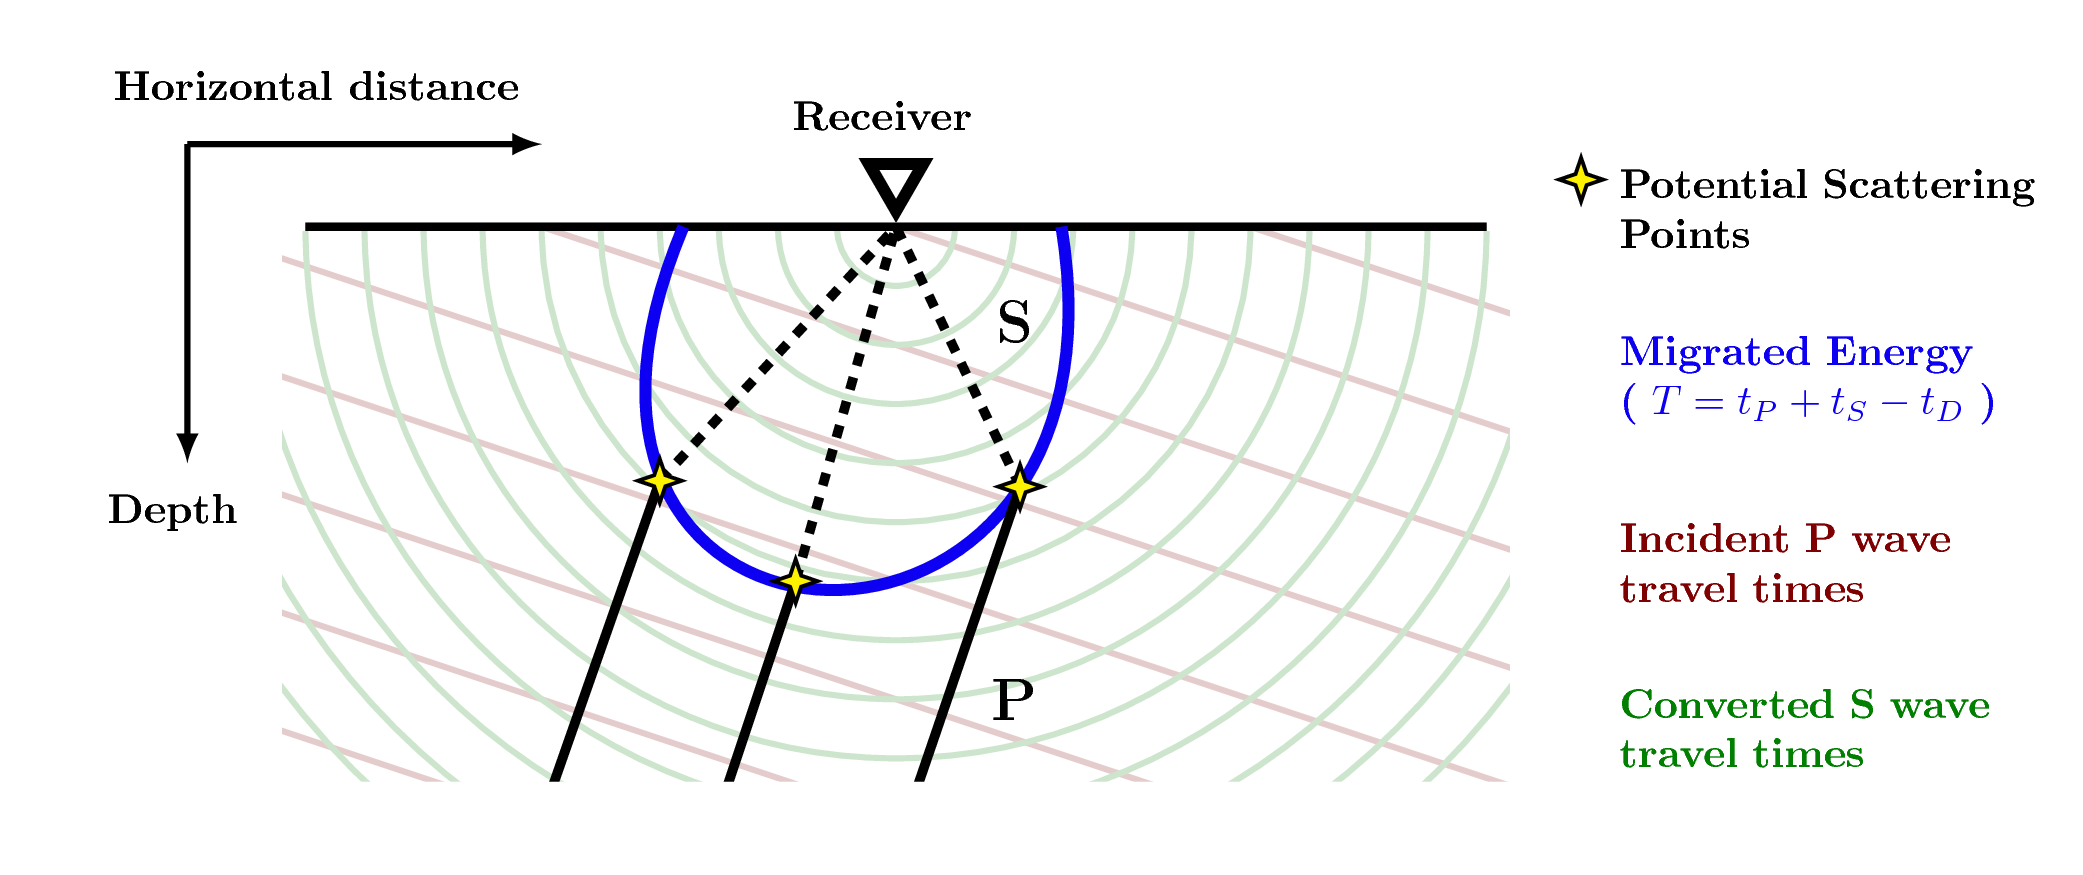
\includegraphics[trim= 0 0 0 0,clip,page=1,scale=.22]
                {../figs/finalfigs/ff1_3.png}
\caption{
Schematic illustration along a 2D profile of the 3D Kirchhoff prestack imaging principle. 
The incoming P-waves (solid lines, red background isochrone lines) and scattered S-waves (dashed lines, green background isochrone lines) arrival times are computed at each grid point in the 3D model box and the energy is migrated (blue curve) along a differential isochron that corresponds to the difference in travel time T between the direct wave ($t_D$) and the P wave to the scatterer ($t_P$) added to the S wave to the receiver ($t_S$). 
This isochron represents all the points in depth in the 3D model space that could account for scattered energy seen at a given time on the RF.
In the 3D case, the isochron extends as an ellipsoid whose shape depends on the source-receiver geometry and the reference velocity model.
}
\end{figure*}
%-----------------------------------------%
%     F     I     G     U     R     E     %
%-----------------------------------------%

% - - - - - -
% Subsection
% - - - - - -
\subsection{Kirchhoff prestack depth migration}

In order to exploit these three-component \hl{RF signals}, we \hl{implement} a prestack migration that allows to naturally take 3D effects into account. % from reflection to transmission seismology. 
Kirchhoff prestack depth migration is a technique that was developed in exploration geophysics and that maps scattered phases observed on seismograms located at the surface back at depth to scattering points \citep{ylma_book_01}.
Using a reference velocity model, the energy is propagated back in depth to all the points in 3D that would provide the same observed arrival.
By doing so, we effectively treat each grid point as a potential scatterer and smear the energy of a given observed arrival along a migration isochron in the depth domain.
The energy at depth for each observed trace is then stacked after migration.
Alternatively, in the data space, \hl{this} corresponds to finding the scattering points or interfaces by stacking the energy peaks along coherent diffraction hyperbolae.
\hl{A visual representation of the Kirchhoff imaging principle in the model space can be found in fig1.}

For two observed phases on two different waveforms corresponding to the same scattering point (i.e. to the same diffraction hyperbola), the depth-migrated isochrons will intersect at the actual scattering point and stack up constructively.
Extending this observation to all the source-receiver couples and all the scattering points, we can see that this depth domain stacking will focus the energy from the isochrons to the actual scattering features.
However, for this method to work correctly, a high density of data is required.
\hl{For teleseismic data, an ideal array would have an inter-station spacing of less than half the depth of the shallowest structure that we are interested in imaging} \citep{rond_agu_05}.
% for apertures on the order of a few hundred kilometers to correctly map lithospheric structures \citep{rond_sgeo_09}.
As summarized in \citet{rond_sgeo_09}, the imaging principle for the teleseismic Kirchhoff prestack depth migration can be written \hl{in general terms} as:

\begin{align}
  f(x) &= \int\!\!\!\!\int \vec{\text{w}}(x,r) \cdot \Delta\vec{\text{u}}(r,t=T(r,x)) \; dr
  \label{gen}
\end{align}
\vspace{1mm}

\noindent where is $f(x)$ the scattering potential at a given image point $x$ in depth, 
$r$ describes the source-receiver geometry on the region of interest, 
the weights $\vec{\text{w}}(x,r)$ are linked to the treatment of the wavefield’s amplitude and polarity during the migration, 
$\Delta\vec{\text{u}}$ is the three-dimensional scattered wavefield obtained through \hl{the multichannel preprocessing approach} described in previous section, 
and $T(r,x)$ represents the arrival times associated with a given \hl{(source - scatterer - receiver)} geometry estimated in a reference 3D velocity model. 
For the forward P-to-S scattering, for example, we have $T(r,x) = t_P + t_S - t_d$, where $t_P$, $t_S$ and $t_d$ are travel times computed in the reference 3D velocity model.
\hl{$t_P$ is the travel time for the P-wave traveling from the source to the scattering point, $t_S$ for the S-wave traveling from the scattering point to the receiver, and $t_d$ for the the direct P-wave traveling from the source to the receiver.} 
We use the fast marching method \citep[FM3D,][]{deko_gji_06} to compute these travel time fields. 
\hl{FM3D solves the Eikonal equation in our 3D space after initializing the teleseismic arrival times at the border of the domain.
It yields the travel-time fields for all the scattered phases, including the free surface multiples, by progatating the wavefield a first time upwards (direct) and a second time downwards (reflected).
It uses this multi-stage approach to obtain all the travel times with only one computation.}
This makes this approach computationally \hl{performant}. 
The integrals are \hl{carried out} over all the sources and receivers.


The weights $\vec{\text{w}}(x,r)$ account for the amplitude of the migrated waveforms. 
They are a linear combination of the geometrical spreading, the scattering patterns and the projection of the incoming polarization vector of the scattered phase on the (R,T,Z) reference frame at the station.
\hl{Note that the reference frame changes for each event.}
The geometrical spreading accounts for amplitude reduction due to 3D wave propagation from the scattering point to the receiver.
The scattering patterns can be seen as simulating the physics of elastic wave propagation (e.g. amplitude of a P-to-S conversion) without having to numerically compute the full wavefield.
Taking those elements into account in the migration allows us to retrieve a greater amount of information from the waveforms \hl{every time than if we were migrating only one component}.

% - - - - - -
% Subsection
% - - - - - -
\subsection{Accounting for scattering theory}

\citet{cheng_gji_16} showed that, in order to image dipping discontinuities for any incoming slowness and back-azimuth, the polarities and amplitudes of the RF need to be corrected by using scattering patterns.
However, the authors used the scattering patterns from \citet{rond_sgeo_09}, which are 3D scattering patterns projected in 2D. 
This approximation is valid for $S_V$ scattered waves that are polarized in the plane defined by the source, the scattering point and the receiver (hereafter called the scattering plane), \hl{and is applicable to the case of forward P-to-S scattering}.
However, in order to treat the $S_H$ \hl{waves generated by scattering of free surface reverberations}, we need to use fully 3D scattering patterns. 

Scattering patterns describe the amplitude and \hl{orientation} of the polarization vector of the wave scattered at any point $x$ \hl{in our 3D model space, for a given source-receiver geometry $r$}. 
That is, for a given angle between the incoming and scattered wave, they give the amplitude and sign of the scattered phase. % (see fig3). 
We compute this value for every $r$ geometry and \hl{each possible scattering point $x$ in our 3D model}.
The projection of the estimated polarization vector from $x$ to the station on the (R,T,Z) reference frame at the station is a measure of how much a scatterer at $x$ would contribute to each component of the RF. 
Applying the dot product between this resulting vector and the observed wavefield $\Delta\vec{\text{u}}(r,t=T(r,x))$  tells us how much energy should be migrated to $x$.

As suggested in \citet{tone_epsl_08}, migrating multiple component RFs improves the final image if polarities are correctly treated.
%Correcting the amplitude and polarities of the scattered waves using scattering theory allows us to retrieve coherent information on all three components of the RF \hl{every time}.
%As in other methods that use three component RFs, this gives rise to three possible situations.
\hl{Using three component RFs gives rise to three possible situations regarding the coherence of the data.}
If a given grid point corresponds to an actual scatterer, we will extract coherent information on the three components of the RF.
If the grid point corresponds to a geometry where no scattering is theoretically expected (e.g. a 180 angle between an incoming P and a scattered S wave), no energy will be migrated from the RF. 
Finally, if the grid point has high potential scattering values but the three components of the RF are not coherent, i.e. there is no scattering at that point, recorded amplitudes will be migrated, but will interfere destructively when stacked together.
This allows us to consistently extract the coherent information of the RF. 
We will now explicitly describe the terms that go into $\vec{\text{w}}(x,r)$ and how we modify the imaging principle to incorporate the free surface multiples.

%-----------------------------------------%
%     F     I     G     U     R     E     %
%-----------------------------------------%
\begin{figure*}[t]
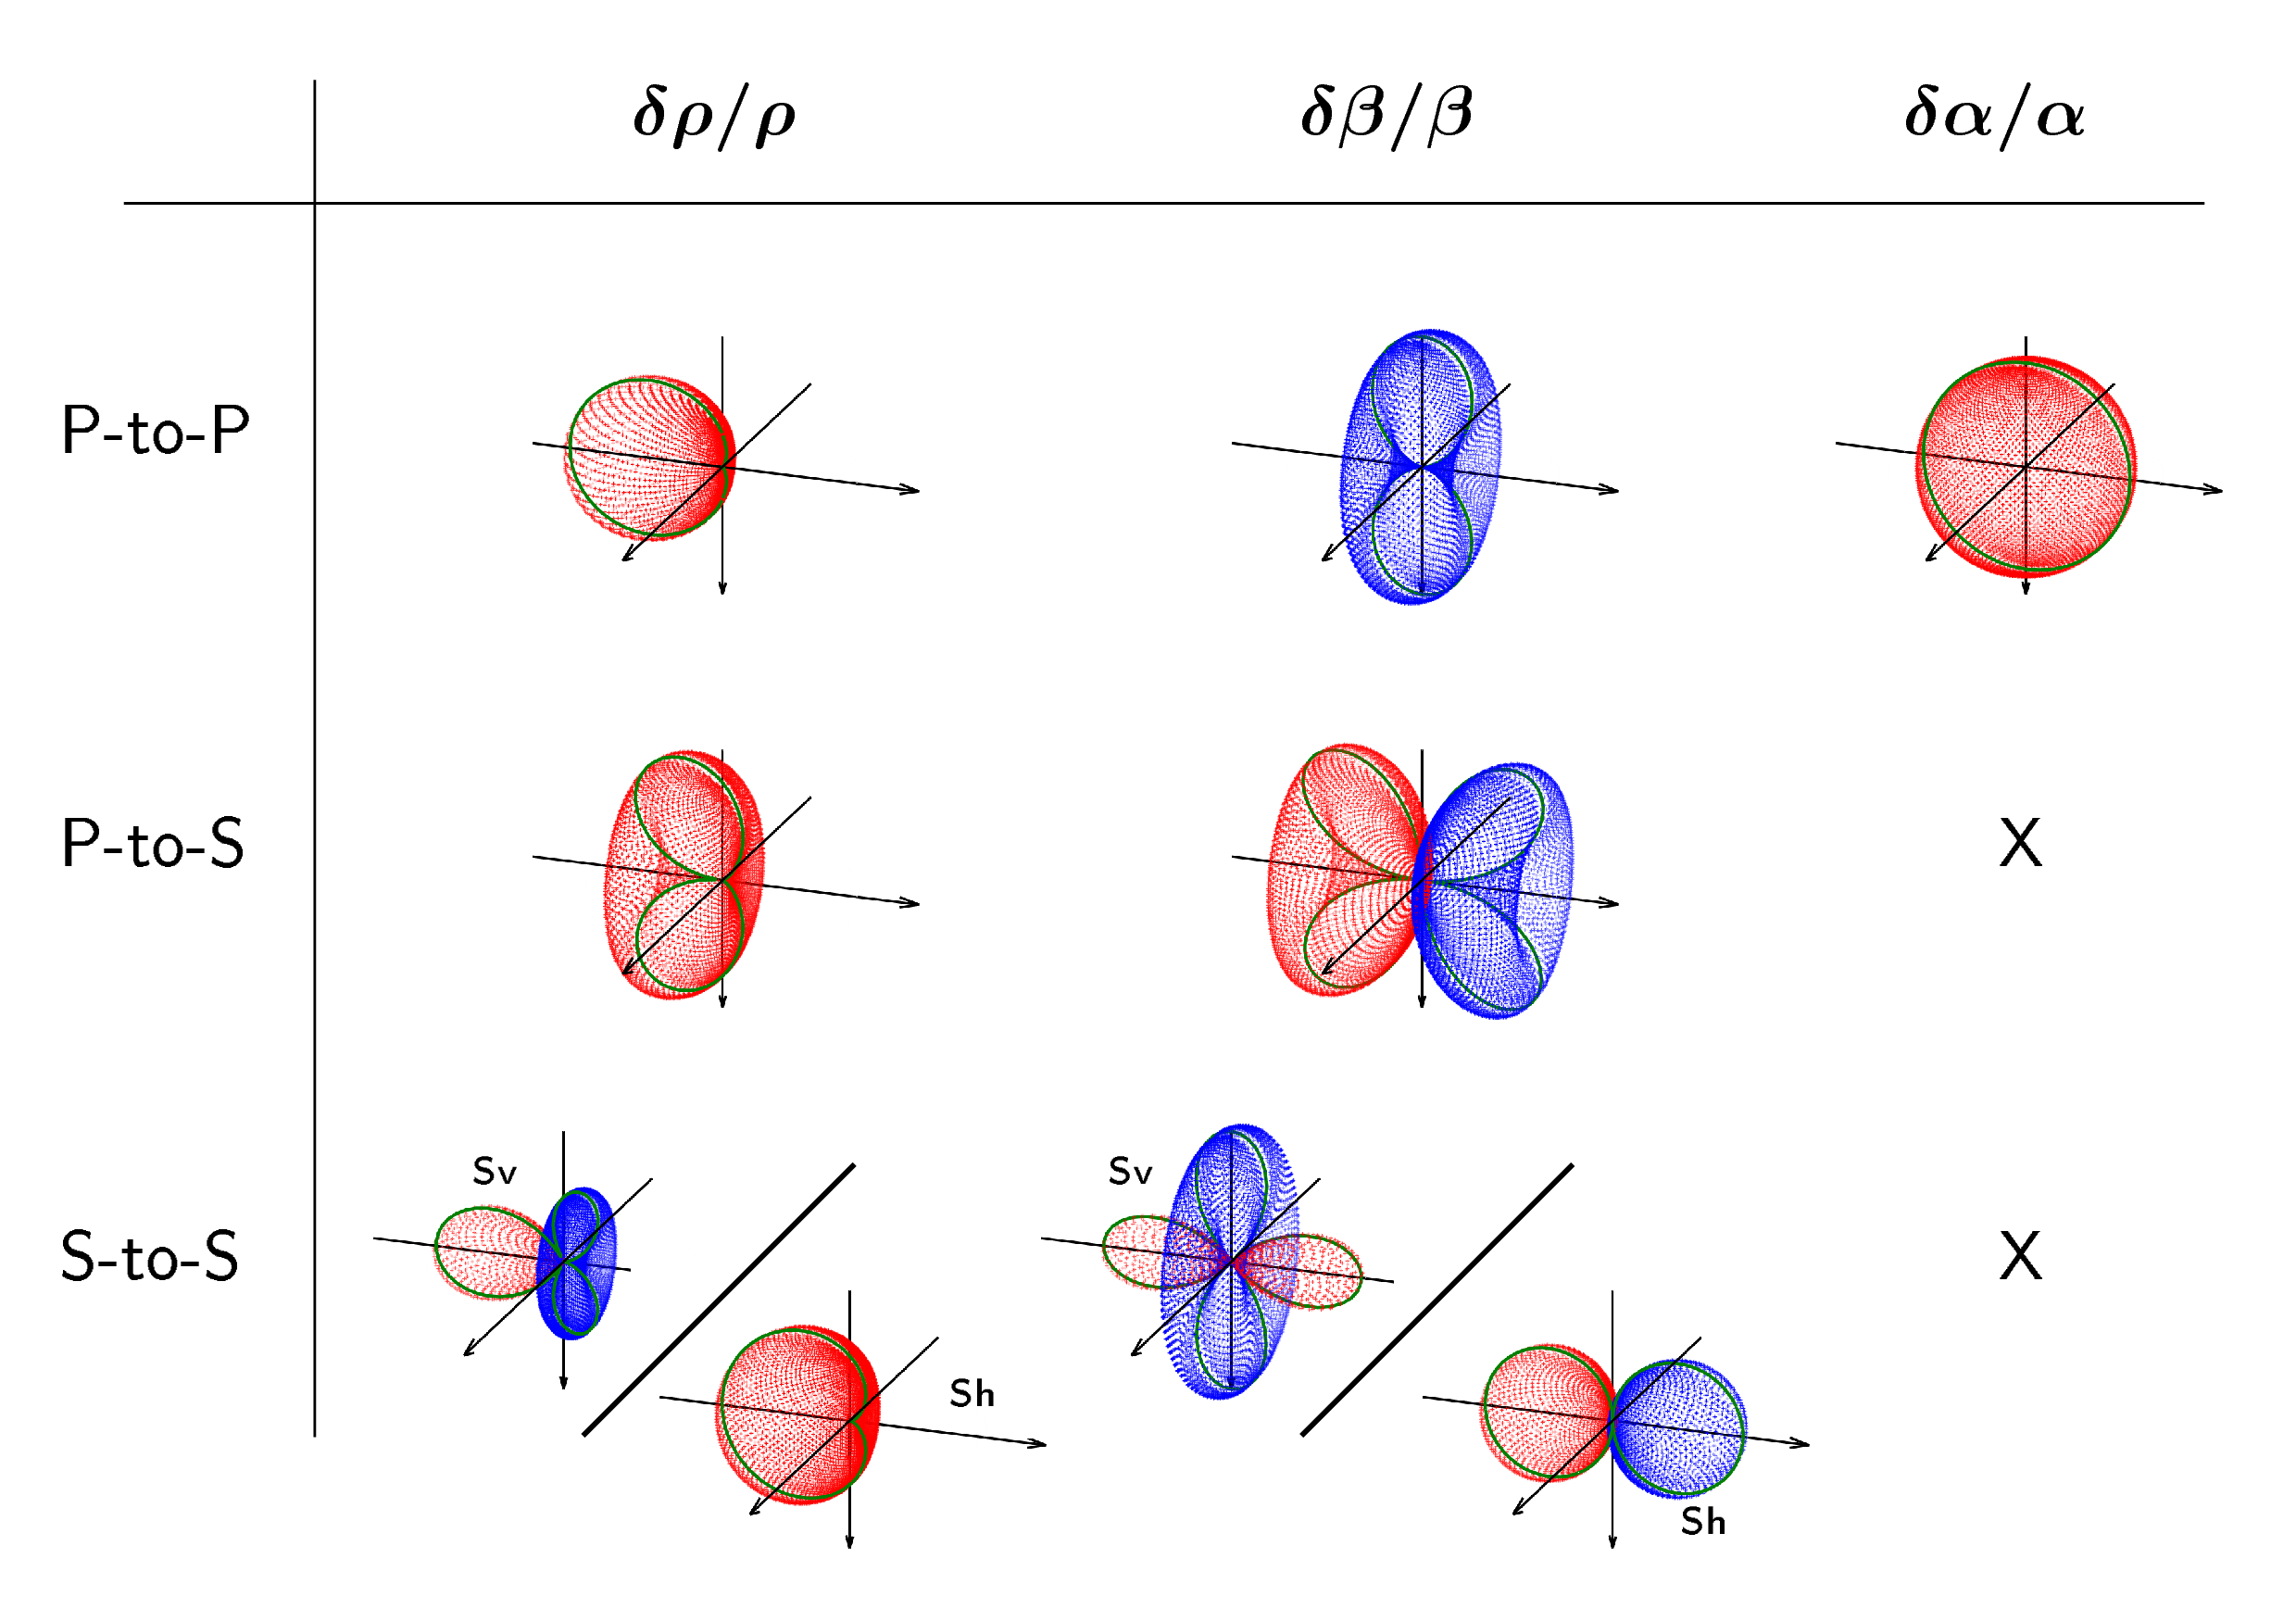
\includegraphics[trim= 0 0 0 0,clip,page=1,scale=.18]
                {../figs/finalfigs/ff2_3.png}
\caption{
Representation of the 3D scattering patterns. 
The incoming wave arrives from the left-handside along the horizontal axis as either a P-wave oscillating rightwards or an S-wave oscillating upwards, and leaves according to the scattering geometry. 
The scattering amplitude is represented as distance to the scattering point (center of each plot) and the polarity is represented by color, red being positive and blue negative. 
Here we can take both forward and back scattering into account. 
All of them are symmetrical with respect to the horizontal incoming wave propagation axis. 
Note that $\rho$ perturbations generate mostly back scattering and $\alpha$-$\beta$ perturbations have equal parts of forward and back scattering. 
The final value for a given scattering geometry is obtained by multiplying the amplitude value by the polarity for that scattering angle.
}
\end{figure*}
%-----------------------------------------%
%     F     I     G     U     R     E     %
%-----------------------------------------%

% - - - - - -
% Subsection
% - - - - - -
\subsection{Three-dimensional scattering patterns}

\hl{Three-dimensional scattering patterns have been derived by a number of authors} \citep[e.g.,][]{wuak_gphy_85,fred_gji_04}. 
\hl{Here we employ the 3D scattering patterns derived for a single scattering point that were obtained by} \citet{beyl_wamo_90}. 
The authors study the behavior of a plane wave propagating in a smooth velocity model that hits a scattering point.
Extending the equations for volumetric scattering to point scattering under the single scattering Born approximation, they express the amplitude and polarization of scattered waves for incoming unit vectors.
This defines the following scattering patterns $\varepsilon^{X_1X_2}$ for any given incident $X_1$ and departing $X_2$ seismic wave at the scattering point:

\begin{align}
  \varepsilon^{pp} (\theta) &= \dfrac{\delta \rho}{\rho_0} 
                               \left( 1 + \cos(\theta) + \dfrac{\beta_0}{\alpha_0} (\cos(2\theta)-1) \right) \notag
                   \\ & \quad + 2 \dfrac{\delta \alpha}{\alpha_0} 
                               + \dfrac{\delta \beta}{\beta_0} \left( 2 \dfrac{\beta_0^2}{\alpha_0^2} (\cos(2\theta)-1) \right)
\\
  \varepsilon^{ps} (\theta) &= \dfrac{\delta \rho}{\rho_0} 
                               \left( \sin(\theta) + \dfrac{\beta_0}{\alpha_0} \sin(2\theta) \right) \notag
                   \\ & \quad + \dfrac{\delta \beta}{\beta_0} \left( 2 \dfrac{\beta_0}{\alpha_0} \sin(2\theta) \right)
\\
  \varepsilon^{sp} (\theta) &= - \varepsilon^{ps}
\\
  \varepsilon^{s_Vs_V} (\theta) &= \dfrac{\delta \rho}{\rho_0} 
                                   \bigg( \cos(\theta) + \cos(2\theta) \bigg) \notag
                       \\ & \quad + \dfrac{\delta \beta}{\beta_0} \bigg( 2 \cos(2\theta) \dfrac{}{} \bigg) 
\\
  \varepsilon^{s_Hs_H} (\theta) &= \dfrac{\delta \rho}{\rho_0} 
                                   \bigg( 1 + \cos(\theta) \dfrac{}{} \bigg)
                                   + \dfrac{\delta \beta}{\beta_0} \bigg( 2 \cos(\theta) \dfrac{}{} \bigg)
\end{align}
\vspace{1mm}

\noindent where $\alpha$ is the P-wave velocity, 
$\beta$ is the S-wave velocity, 
$\rho$ is the density, 
subscript $\cdot_0$ corresponds to the smooth reference model, 
$\delta$ corresponds to the local heterogeneity at the scattering point and 
$\theta$ is the scattering angle between the incoming $X_1$ phase and the $X_2$ scattered phase in the scattering plane at the scattering point.
\hl{A visual representation of the 3D scattering patterns can be found in fig2.}
Here, we note that $S_V$ is defined locally at the scattering point and is the part of the S-wave that oscillates in the scattering plane, not in the great-circle plane.
Conversely, $S_H$ oscillates orthogonally to the scattering plane.

\hl{However, in the scope of this article, we will not be taking the full scattering patterns into account.
Because our migration method does not rely on an inversion, we cannot easily mitigate the contributions of variations in $\rho$, $\alpha$ and $\beta$ for our scattering modes} \citep{cheng_gji_16}.
\hl{Because variations in density generate almost only back-scattering, we don't consider its influence in the forward PS mode scattering, i.e. we say that $\delta\rho / \rho = 0$.}
\hl{Also, we decide to only take variations in seismic velocities into account in the free surface multiples to stay coherent with the PS mode.
This means that we will only take $\beta$ variations into account when considering P-to-S or S-to-S scattering and $\alpha$ variations for P-to-P scattering.
This is an arbitrary choice, and although some of the back-scattering recorded on the waveforms will be due to density variations, removing $\rho$ from the equations will allow for more coherent interpretations of the stacked migrated images.
This will be represented by subscript $\cdot_{\beta}$ and $\cdot_{\alpha}$ respectively hereafter.}

In this work, we obtain the scattering angle by estimating the directions of propagation of the incoming and scattered waves at the grid point.
These directions are given by the gradient of the wavefront obtained from the Eikonal solver.
The angle $\theta$ is then used to compute the scattering patterns, and characterizes the behavior of every scattered phase.

Once we obtain the scattering with the angle $\theta$ and estimate the polarization of the scattered wave, we project this vector on the (R,T,Z) reference frame at the station.
\hl{The level of fit between observed and predicted measurements is measured by computing the dot product of the recorded energy vector $\Delta\vec{\text{u}}(r,t=T(r,x))$ and the predicted energy vector $\vec{\text{w}}(x,r)$ from the surface projection. 
This tells us how much energy scattered at point $x$ is expected to contribute to each component of the RF, and defines the level of energy that is migrated to depth.}

% - - - - - -
% Subsection
% - - - - - -
\subsection{Forward scattered waves and free surface back-scattered multiples}

Standard RF studies interpret the phases observed in deconvolved waveforms only as forward P-to-S conversions, referred to as PS hereafter, although a well-known issue is the influence of the free surface multiples.
\hl{Interferences} from these scattered phases \hl{stack up at spurious depths}, and can generate serious artifacts that hinder the interpretation of features in the migrated images \citep{cheng_grl_17}.
However, if properly accounted for, multiple reflections can become a useful tool as they bring complementary information about the structure \citep{tauz_epsl_16}. 

The free surface multiples are the waves that reflect at the free surface of the Earth and are backscattered towards the surface by the same heterogeneities that generate the direct PS scattering.
In the case of the Born approximation, we are looking at three different multiple modes. % (see fig3).
The first one to arrive is reflected as a P wave at the surface, hereafter referred to as lower case p, and backscattered as a P wave.
The second one is also reflected as a P wave but backscattered as an S wave towards the station.
The third one is reflected as a converted S wave at the surface, hereafter refered to as lower case s, and backscattered as an S wave.
These phases will be referred to as PpP, PpS and PsS respectively.
Note that the S-to-S scattering for the PsS wave has as both an $S_V$-to-$S_V$ and an $S_H$-to-$S_H$ component.
%A visual representation of these phases is shown in the first column of fig3.

\hl{In the next section} we will show how we also account for phases reflected at the surface, i.e. PpP, PpS and PsS modes of scattering in the migration algorithm.
Let us first write the imaging principle in the case of forward PS scattering mode.
Since we work with a finite the number of sources $i$ and stations $j$, and use a finite number of grid points $k$, equation eq.\eqref{gen} can be rewritten in the discrete form:

\begin{align}
  f_{ps}(k) &= \sum_i \sum_j \; \text{G}(j,k) \; \varepsilon^{ps}(i,j,k) \; \notag\\&\qquad\qquad \vec{\delta}_{ps}(j,k) \cdot \Delta\vec{\text{u}}(i,j,t_P+t_S-t_d)
 \label{ps}
\end{align}
\vspace{1mm}

\noindent where $f_{ps}(k)$ is the scattering potential for the forward PS scattering mode at a given grid point $k$,
G$(j,k) = 1 / dist(j,k)$ is the amplitude correction for geometrical spreading with $dist(j,k)$ the distance between the receiver and the scatterer, 
$\varepsilon^{ps}$ is the scattering pattern for the PS mode, 
and $\vec{\delta}_{ps}$ is a unit vector representing the polarization of the scattered S-wave.
Finally, $t_P$, $t_S$ and $t_d$ are travel times computed in the reference 3D velocity model \hl{described in the previous section}. % for the P-wave traveling from the source to the scattering point, the S-wave traveling from the scattering point to the receiver, and the direct P-wave traveling  from the source to the receiver respectively.
We use the fast marching method \citep[FM3D,][]{deko_gji_06} to compute these travel time fields.

%-----------------------------------------%
%     F     I     G     U     R     E     %
%-----------------------------------------%
\begin{figure*}[t]
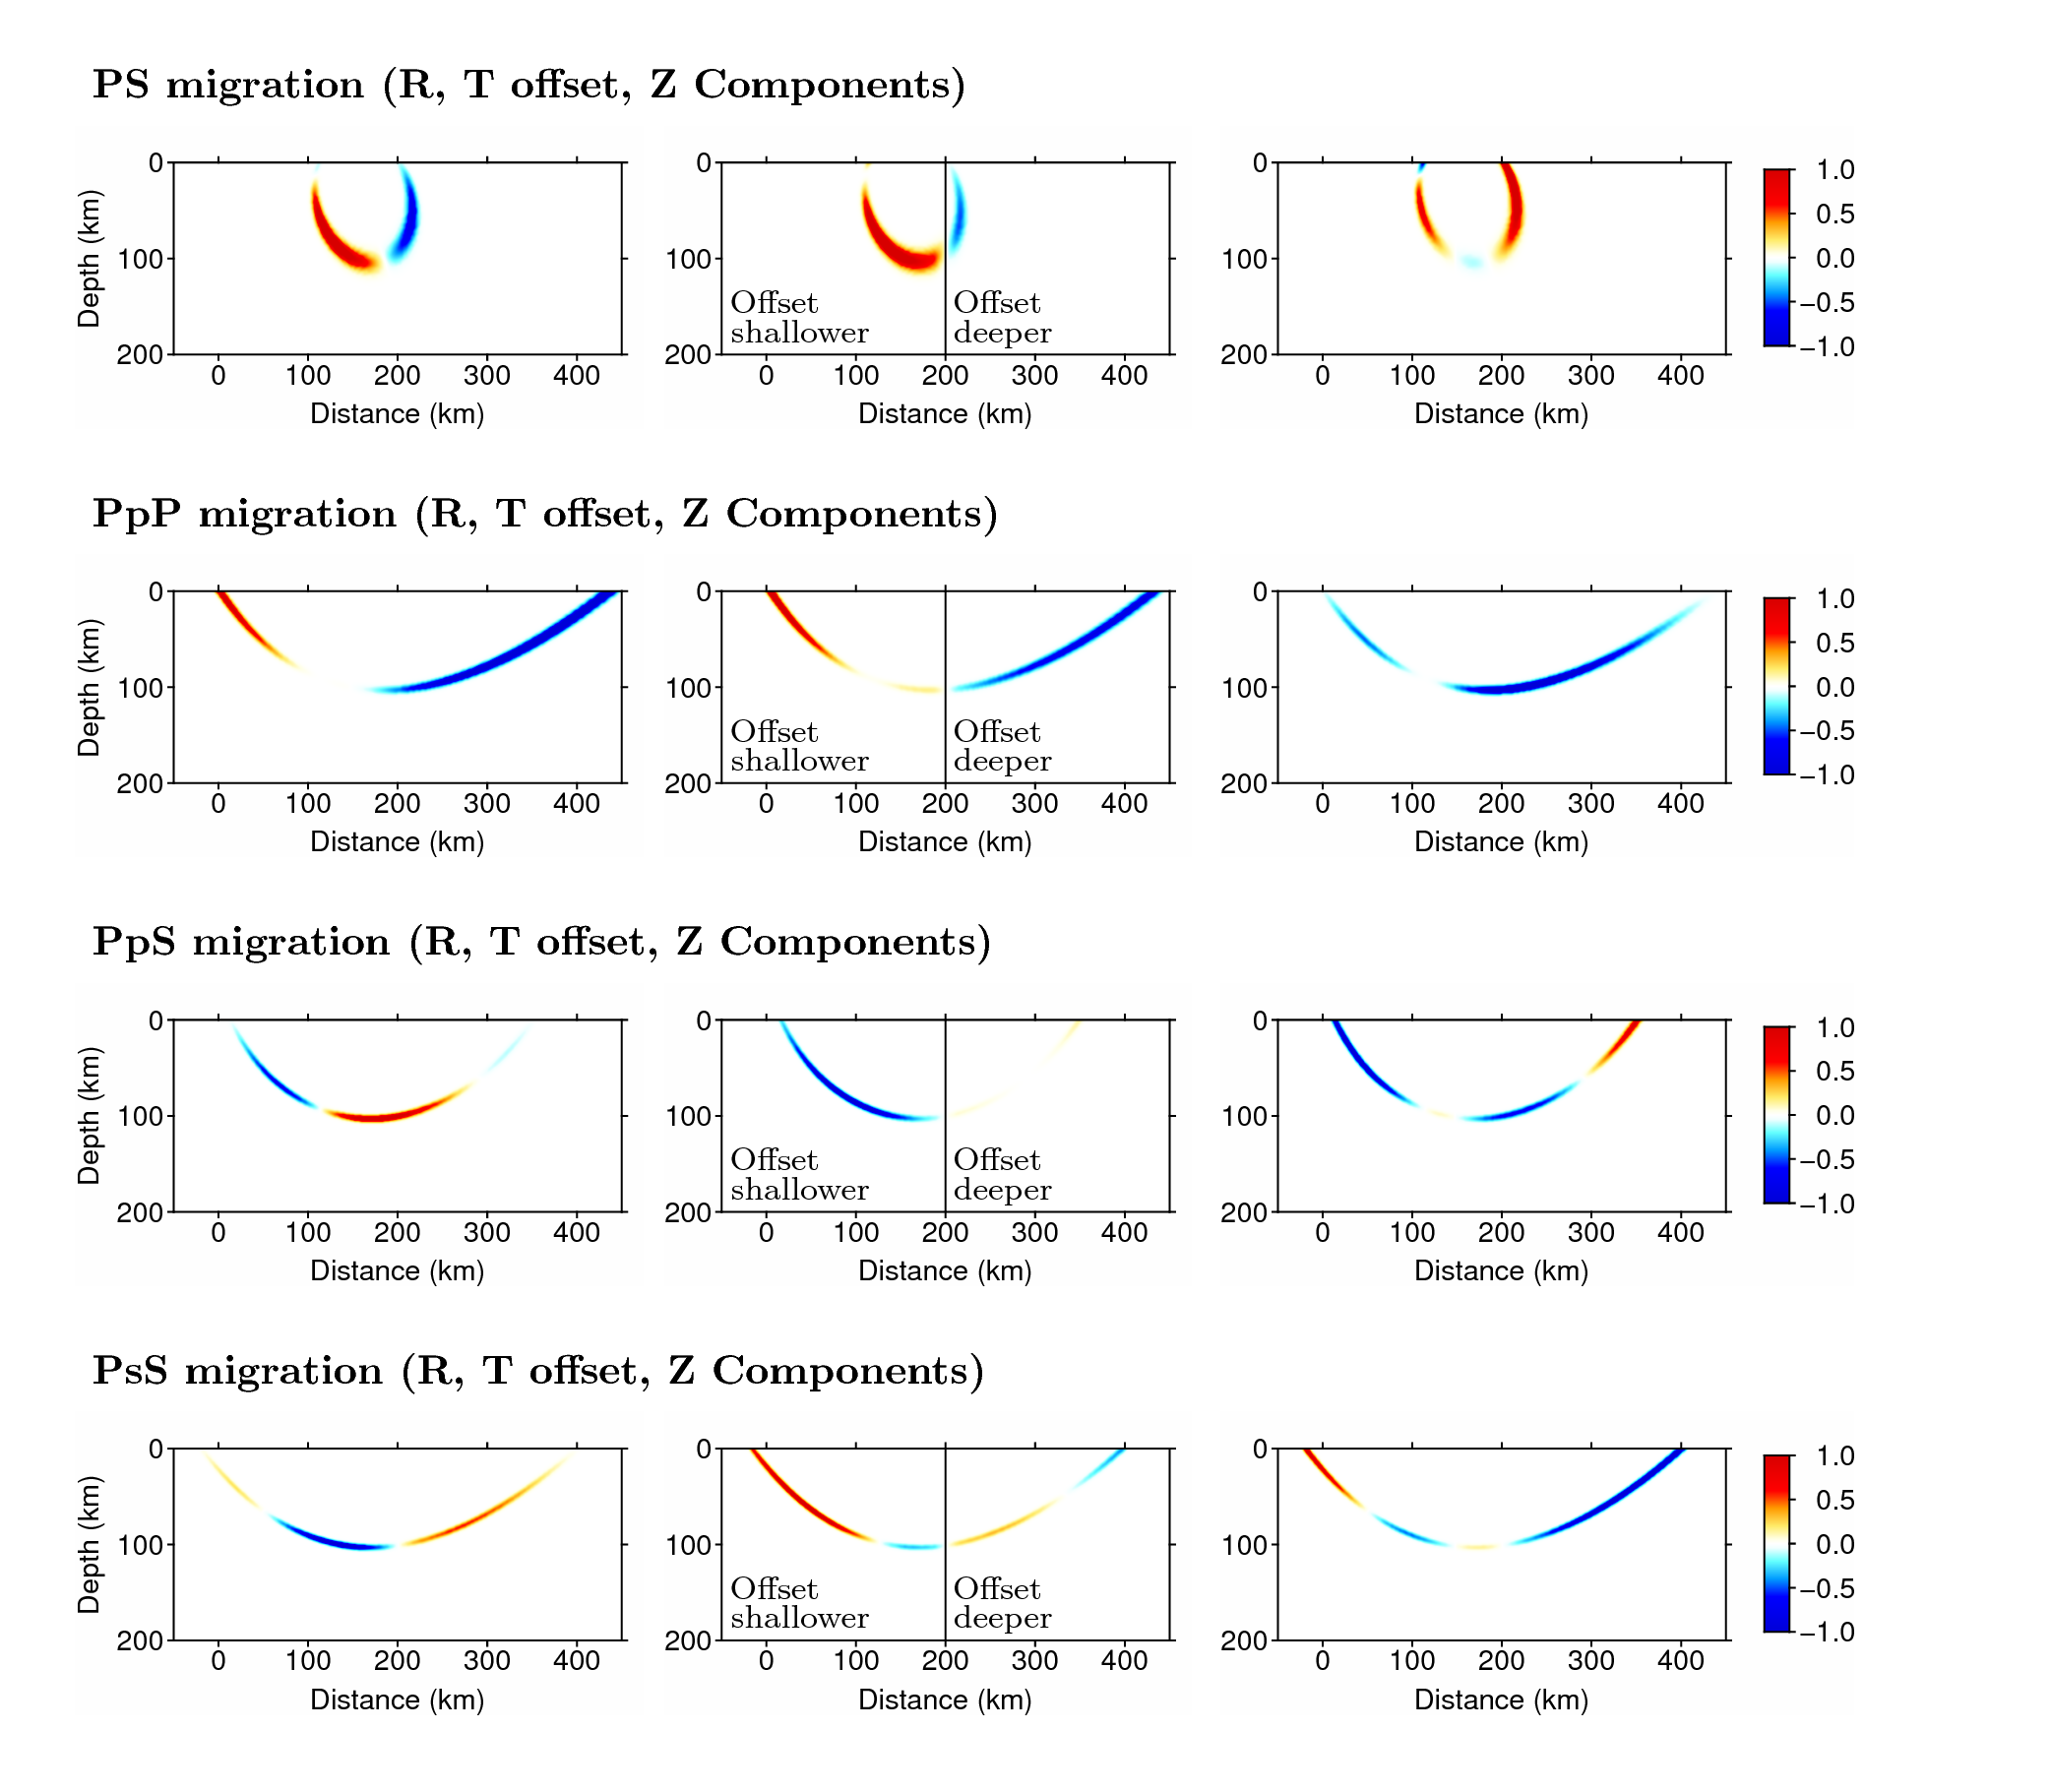
\includegraphics[trim= 0 0 0 0,clip,page=1,scale=.22]
                {../figs/finalfigs/ff3_3.png}
\caption{
2D representation of the complete scattering weights without focussing for the four scattering modes and the three components migration. 
The row correspond to a given scattering mode and the columns correspond to the three components of the recorded wavefield.
For the transverse component, because its amplitude is null along the great circle plane, the slice through the 3D model is offset shallower (towards the reader) or deeper (away from the reader) to visualize its amplitude and polarity behaviour better.
This is what generates the visible polarity reversals at 200km.
They are obtained by migrating a unit gaussian peak along the isochron for a given scattering mode for a source that arrives under the station from the right-handside. 
They correspond to the projection of the weights from the scattering patterns at the surface for each recorded component, with blue corresponding to a polarity reversal and red to a preserved polarity.
}
\end{figure*}
%-----------------------------------------%
%     F     I     G     U     R     E     %
%-----------------------------------------%

% - - - - - -
% Subsection
% - - - - - -
\subsection{Integration of free surface multiples}

In order to incorporate the other modes of scattering in the migration and map their energy back at the correct location, we need to compute their associated travel times and amplitudes corrections.
\hl{Specifically}, we need to compute the travel times for the initial P-wave from the source to the surface, the reflected downward going P and S-waves and the back-scattered P and S-waves from all the grid points to the receivers.
Again, we use the fast marching method to compute three travel time fields (P, Ps and Pp) for each source and two (upgoing P and S) for each receiver.
By combining these Pp and Ps travel times with the P and S scattered wave travel times we get the travel times for all 3 first order free surface multiples. 

We use the scattering patterns detailed above to get the correct amplitudes and polarities for these modes as well.
However, in the case of the free surface multiples, the behavior of the amplitude and polarity of the phases is more complex than a single scattering pattern.
In this case, we combine the appropriate $\varepsilon^{X_1X_2}$ scattering patterns in a phase specific complete scattering pattern $S_m$, where $m$ represents one of the four scattering modes.
\hl{We effectively treat the multiples as a double scattering problem with one of the scattering being a reflection at the free surface of the Earth and the other the scattering at depth.}
The expressions for all the $S_m$ can be found hereafter and illustrated along migration isochrons in fig3:

\begin{align}
S_{ps}  &= \varepsilon^{ps}_{\beta}  (\theta)
\\
S_{ppp} &= \varepsilon^{pp}_{\alpha} (\theta') \; \varepsilon^{pp}_{\alpha} (\theta)
\\
S_{pps} &= \varepsilon^{pp}_{\alpha} (\theta') \; \varepsilon^{ps}_{\beta} (\theta)
\\
S_{pss} &= \varepsilon^{ps}_{\beta}  (\theta') \; \Big( (\vec{\delta'} \cdot \vec{\delta}) \; \varepsilon^{s_Vs_V}_{\beta} (\theta)
      \notag \\ & \qquad\qquad\!\! + (\vec{\delta'} \cdot \vec{\gamma}) \; \varepsilon^{s_Hs_H}_{\beta} (\theta) \Big)
\end{align}
\vspace{1mm}

\hl{For the PS scattering this simply corresponds to the direct scattering pattern restricted to the $\delta\beta/\beta$ contribution.}
As opposed to the direct PS scattering mode, \hl{there are two scattering angles to consider for the multiples.}
The first one is the angle $\theta'$ at the free surface reflection, \hl{which} is in the great circle plane that contains the source and the scattering point.
The second one is the angle $\theta$ at the scattering point, \hl{which} is in a second scattering plane defined by the free surface reflection point, the scattering point and the receiver.
\hl{Moreover, for the S-to-S scattering in the PsS scattering mode, we have to consider the polarization of the wave.
In this case, $\delta'$ is the polarization of the wave that is reflected at the surface along the great circle path.
This reflected wave is scattered partly as an $S_V$ wave along $\delta$ and partly as an $S_H$ wave along $\gamma$, that is orthogonal to $\delta$.}
This leads to a generalized definition of the imaging principle, derived from equation eq.\eqref{ps}, for every scattering mode:

\begin{align}
  f_{m}(k) &= \sum_i \sum_j \; \text{G}(j,k) \; \text{S}_{m}(i,j,k) \; \notag\\&\qquad\qquad \vec{\delta}_{m}(j,k) \cdot \Delta\vec{\text{u}}(i,j,T_m)
  \label{mod}
\end{align}
\vspace{1mm}

\noindent where $f_{m}(k)$ is the scattering potential for the scattering mode $m$ at the grid point $k$, 
$m$ $\in [1,4]$ representing one of the four the scattering modes (either PS, PpP, PpS, PsS), 
S$_m(i,j,k)$ is the complete scattering pattern for a given $m$ mode, 
$\vec{\delta}_m(j,k)$ is the unit polarization vector of the scattered wave arriving at the receiver for a given $m$ mode, 
and $T_m$ corresponds to the travel time estimated in a reference 3D model  for a given $m$ scattering mode.
\hl{In the case of} the PpP phase, this corresponds to $T_{PpP} = t_P(i,x') + t_p(x',x) + t_P(x,j) - t_d$ with $x'$ \hl{denoting} the surface reflection point and $x$ the potential scattering point.

\hl{Since} estimating the exact direction of polarization $\vec{\delta}_m(j,k)$ of the scattered wave at the receiver \hl{requires considerable} extra computational cost, here we assume that the polarizations do not change from the scattering point $k$ to the receiver $j$ at the surface.
This is equivalent to assuming straight rays in a homogeneous medium from the scattering point $k$ to the receiver $j$.
\hl{It is a reasonable} approximation for lithospheric and upper mantle \hl{investigations} but may \hl{represent an oversimplification} for lower mantle studies\hl{, where the variations in elastic property bend the rays significantly before they reach the surface.}

%In addition to that, we down-weight the contribution of grid-points that are far on the sides, not exactly below the stations.
\hl{An additional weight is applied to the data in order to limit the contribution of long distance interactions at shallow depths as they leak significant amounts of energy into the images above the region of interest and blur the images.
This means that we effectively put a sensitivity region below the receivers that minimizes the arrivals with low incidence angles.}
\citet{cheng_gji_16} proved that this kind of sensitivity function helps remove artifacts in the migrated images.
However, this means that we limit our ability to image steeply dipping reflectors.
For the PS migration, this limits the \hl{dip of recoverable structures} to 45$^{\circ}$, and for the free surface multiples it means that we loose sensitivity above $\sim$30$^{\circ}$ dip.
%We use a $\cos^4$ as it has very sharp edges at 45$^{\circ}$.
%This leads to the definition of the following imaging principle:
\hl{To down-weight our data, we use a 4\textsuperscript{th} power cosine function of the incidence angle that provides a sharp roll-off at an angle of 45$^{\circ}$, leading to the following updated expression for our imaging principle:}

\begin{align}
  f_{m,foc}(k) &= \sum_i \sum_j \; \text{F}(j,k) \; \text{G}(j,k) \; \text{S}_{m}(i,j,k) \; \notag\\&\qquad\qquad \vec{\delta}_{m}(j,k) \cdot \Delta\vec{\text{u}}(i,j,T_m)
  \label{foc}
\end{align}
\vspace{1mm}

\noindent where $f_{m,foc}(k)$ is the focused scattering potential for the scattering mode $m$ at the grid point $k$, $F(j,k)$=$\cos^4(\nu)$ is the focusing factor and $\nu(j,k)$ is the \hl{incidence angle of the scattered wave} under the station.
This factor can be set to 1 if one wants full coverage of possible dip angle resolution.

Using this imaging principle we get four separate images, one for each scattering mode.
In every image, the energy migrated from the waveforms due to one of the scattering mode is back propagated at the correct depth, while the other three modes are migrated at spurious depths.
However, the benefit of this approach is that these spurious features are migrated at different positions in each image, whereas real structure will be at coherent depths over all modes.
This means that extracting the coherent information between these four images \hl{should penalize against spurious features and enhance true structures.}%, the spurious features should mainly disappear and only let the true structure appear.

%-----------------------------------------%
%     F     I     G     U     R     E     %
%-----------------------------------------%
\begin{figure*}[t]
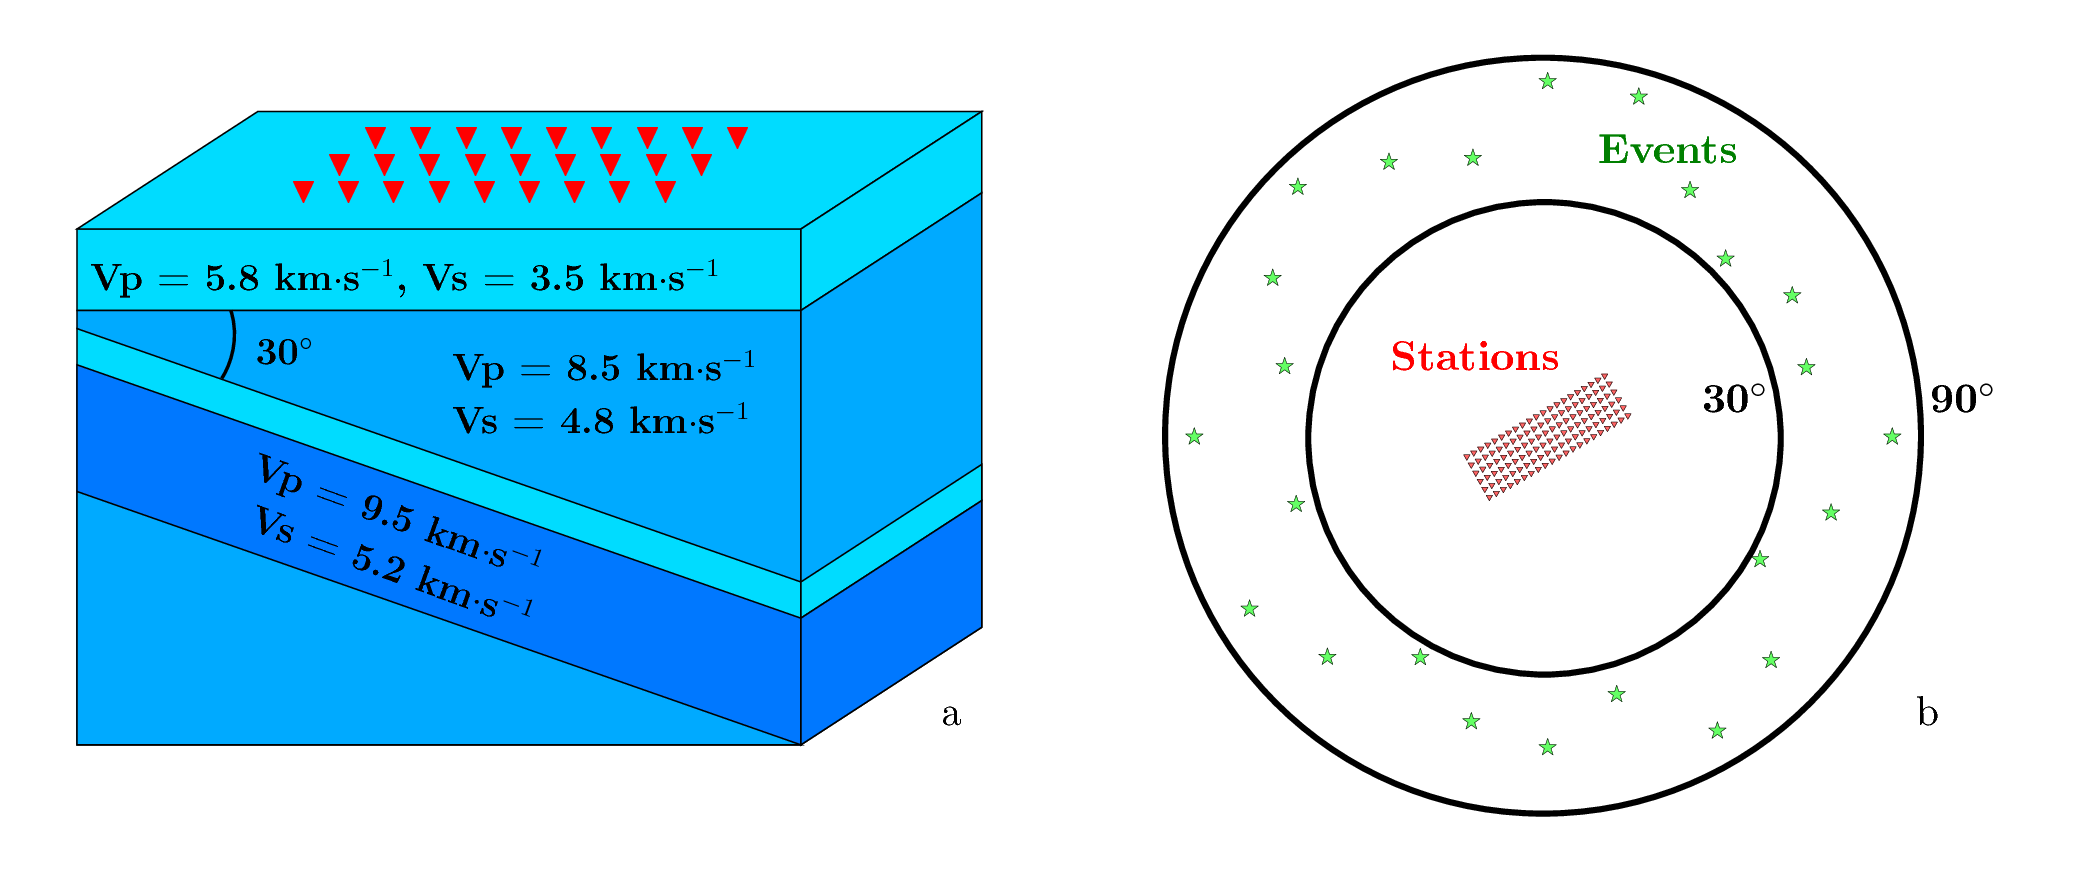
\includegraphics[trim= 0 0 0 0,clip,page=1,scale=.22]
                {../figs/finalfigs/ff4_3.png}
\caption{
Synthetic setup for the tests in figures 5 to 9. 
Red triangles represent the stations in the array and green stars represent the events. 
The array is elongated in the along-dip direction and the sources are evenly spaced in backazimuth and assigned a random epicentral distance from 30$^{\circ}$ to 90$^{\circ}$. 
(a) is a bloc diagram that represents the velocity model for figure 9 (cf. Table 1). 
(b) is a map view of the array and shows the event distribution for the tests performed in figures 7 to 9.
For enhanced clarity only half the rows and half the columns of the array are represented.
}
\end{figure*}
%-----------------------------------------%
%     F     I     G     U     R     E     %
%-----------------------------------------%

% - - - - - -
% Subsection
% - - - - - -
\subsection{Image Stacking Techniques}

\hl{Three stacking techniques are implemented and tested: linear stacking, phase-weighted stacking, and 2\textsuperscript{nd} root stacking.
The following sections describe each of these techniques.}

%  -  -  -  -  -
% Subsubsection
%  -  -  -  -  -
\subsubsection{Linear stacking}

%In order to extract coherent information from multiple images modes, we explored several stacking methods.
%We have implemented three stacking techniques.
The first stacking technique is a linear stack over the four modes can be summarized in the following equation:

\begin{align}
  f_{lin}(k) &= \sum_m \sum_i \sum_j \; \text{F}(j,k) \; \text{G}(j,k) \; \text{S}_{m}(i,j,k) \; \notag\\&\qquad\qquad \vec{\delta}_{m}(j,k) \cdot \Delta\vec{\text{u}}(i,j,T_m)
  \label{lin}
\end{align}
\vspace{1mm}

\noindent where $f_{lin}(k)$ is the stacked scattering potential for all 4 modes at the grid point $k$. 

As \hl{expected}, this \hl{stacking scheme will enhance} the features that are coherent across all four modes.
\hl{However} since the sum is linear, we also expect the spurious features to be reduced by less than an order of magnitude if all modes have roughly the same migrated amplitude.
\hl{This means that the spurious features} will still be visible on the final image.

%  -  -  -  -  -
% Subsubsection
%  -  -  -  -  -
\subsubsection{Phase-Weighted stacking}

The second \hl{technique we consider} is phase-weighted stacking (PWS).
In this approach, we compute the instantaneous phase $\varphi(t)$ of the \hl{input RF signals based on their analytical signals} \citep{schi_gji_97,cost_gphy_18}.
We then migrate and stack the complex phase $e^{i\varphi_k(x)}$ at each grid point, and take the norm of the stacked complex phase as a measure of the coherence \citep{coop_saga_07}.
This can be summarized in the following general equation:

\begin{align}
  y(x) &= \dfrac{1}{N} \sum_j^N s_j(x) \left\vert \dfrac{1}{N} \sum_k^N e^{i\varphi_k(x)} \right\vert
  \label{pws_1}
\end{align}
\vspace{1mm}

\noindent where the first sum represents the amplitude stack of the data $s_j$,
the second sum is the norm of the stacked unit migrated complex phases $e^{i\varphi_k}$ that acts as a filter to the amplitude stack,
\hl{and $y(x)$ is the stacked migrated signal}.
On one hand, if the signals are coherent, their instantaneous phases $\varphi_k$ will point in the same direction and the modulus of the sum of the complex phases will be high.
On the other hand, if the signals at a given grid point \hl{consists mainly of noise}, then the instantaneous phases will point towards random directions and cancel out, leading to a minimum in the \hl{modulus of the} stacked complex phases.

In our case, we need to compute the instantaneous phase of the 3D incoming signal using the estimated polarization of the scattered waves, which is different at every grid point, based on the instantaneous phase of the three components of the RF.
This leads to \hl{a reformulation of} our imaging principle as follows:

\begin{align}
  f_{pws}(k) &= \text{C}(k) \; \sum_m \sum_i \sum_j \; \text{F}(j,k) \; \text{G}(j,k) \; \text{S}_{m}(i,j,k) \; \notag\\&\qquad\qquad\qquad \vec{\delta}_{m}(j,k) \cdot \Delta\vec{\text{u}}(i,j,T_m)
  \label{pws}
\end{align}
\vspace{1mm}

\noindent where $f_{pws}(k)$ is the phase-weighted stacked scattering potential for all 4 modes at the grid point $k$.
C$(k)$ is the coherence of the four modes defined as:

\begin{flalign}
  & \qquad\qquad\quad\!\!   \qquad\qquad\qquad\qquad\qquad\qquad
    \text{C}(k) = \left\vert \sum_m \sum_i \sum_j e^{i\varphi(m,i,j,k)} \right\vert &
    \label{coh}
\\
  & \text{with} \qquad\qquad   \qquad\qquad\qquad\qquad\qquad\qquad
    \varphi = arg( \text{S}_m \; \vec{\delta}_m \cdot \Delta\tilde{\text{u}}) &
    \label{arg}
\end{flalign}
\vspace{1mm}

\noindent where $\Delta\tilde{\text{u}}$ is the analytical signal of $\Delta\vec{\text{u}}$.
%As the name implies, the Phase-Weighted stack is a phase coherence filter that we apply directly to the linear migration.

%  -  -  -  -  -
% Subsubsection
%  -  -  -  -  -
\subsubsection{2\textsuperscript{nd} root stacking}

Finally, we \hl{consider} a 2\textsuperscript{nd} root stacking technique based on \citet{schi_gji_97}.
This is \hl{a non-linear stacking method that sums} the square root of the amplitudes for all the traces and takes the resulting image to the power 2 after the stack.
The general formula for N\textsuperscript{th} root stacking can be summarized as follows:

\begin{flalign}
  & \qquad\qquad\!   \qquad\qquad\qquad\qquad\qquad\qquad
    y(x) = sign\big(r(x)\big) \; \vert r(x) \vert^{n} &
    \label{2nd_1}
\\
  & \text{with} \qquad   \qquad\qquad\qquad\qquad\qquad\qquad
    r(x) = \dfrac{1}{N} \sum_j^N sign\big(s_j(x)\big) \; \vert s_j(x) \vert^{1/n} &
    \label{2nd_2}
\end{flalign}
\vspace{1mm}

\noindent where $r(x)$ is the stack of the N\textsuperscript{th} roots of the $s_j(x)$ data,
\hl{and $y(x)$ is the final stacked migrated signal taken to the N\textsuperscript{th} power}.
We tried other power values for the N\textsuperscript{th} root stacking method but higher values tend to remove everything but the sharpest coherent contrasts, which can be problematic for smaller coherent scattering structures.

In our case, if we \hl{assign the variable} $\mathcal{A}(i,j,k)$ to the corrected amplitude for every $(i,j,k)$ triplet and \hl{the variable} $\mathcal{S}(k)$ to the value of the stacked square root of the amplitudes at grid point $k$, we can rewrite our imaging condition as:

\begin{align}
  f_{2rs}(k) &= sign(\mathcal{S}(k)) \left\vert \sum_m \sum_i \sum_j \; sign(\mathcal{A}(i,j,k)) \; \right.\notag\\&\qquad\left. \Big\vert \text{F}(j,k) \; \text{G}(j,k) \tfrac{}{}\; \text{S}_{m}(i,j,k) \; \right.\notag\\&\qquad\qquad\left. \vec{\delta}_{m}(j,k) \cdot \Delta\vec{\text{u}}(i,j,T_m)\Big\vert^{1/2} \right\vert ^2
  \label{2rs}
\end{align}
\vspace{1mm}

\noindent where $f_{2rs}(k)$ is the 2\textsuperscript{nd} root stacked scattering potential for all 4 modes at the grid point $k$.
%This time, as opposed to the Phase-Weighted stack, we obtain an efficient amplitude coherence filter with this definition of the 2\textsuperscript{nd} root stack.

In the \hl{current} section we described the physics and the geometry of the problem with the scattering patterns.
\hl{We} explicitly described the equations and the imaging principles we need to obtain the final stacked images of the subsurface.
In \hl{what follows}, we use synthetic examples to show that the resulting imaging principle (eq.\eqref{foc}) is robust, and that we are able to \hl{integrate all the available data in the analysis without} back-azimuth or slowness restrictions.
Then we show how the different stacking methods affect the results, and \hl{finally we discuss the computational efficiency of the method and apply the imaging principles to real data}. 


%---------
% Section
%---------
\section{Synthetic tests}

% - - - - - -
% Subsection
% - - - - - -
\subsection{Model and setup}

%-----------------------------------------%
%     T     A     B     L     E     S     %
%-----------------------------------------%
\begin{table*}[t]
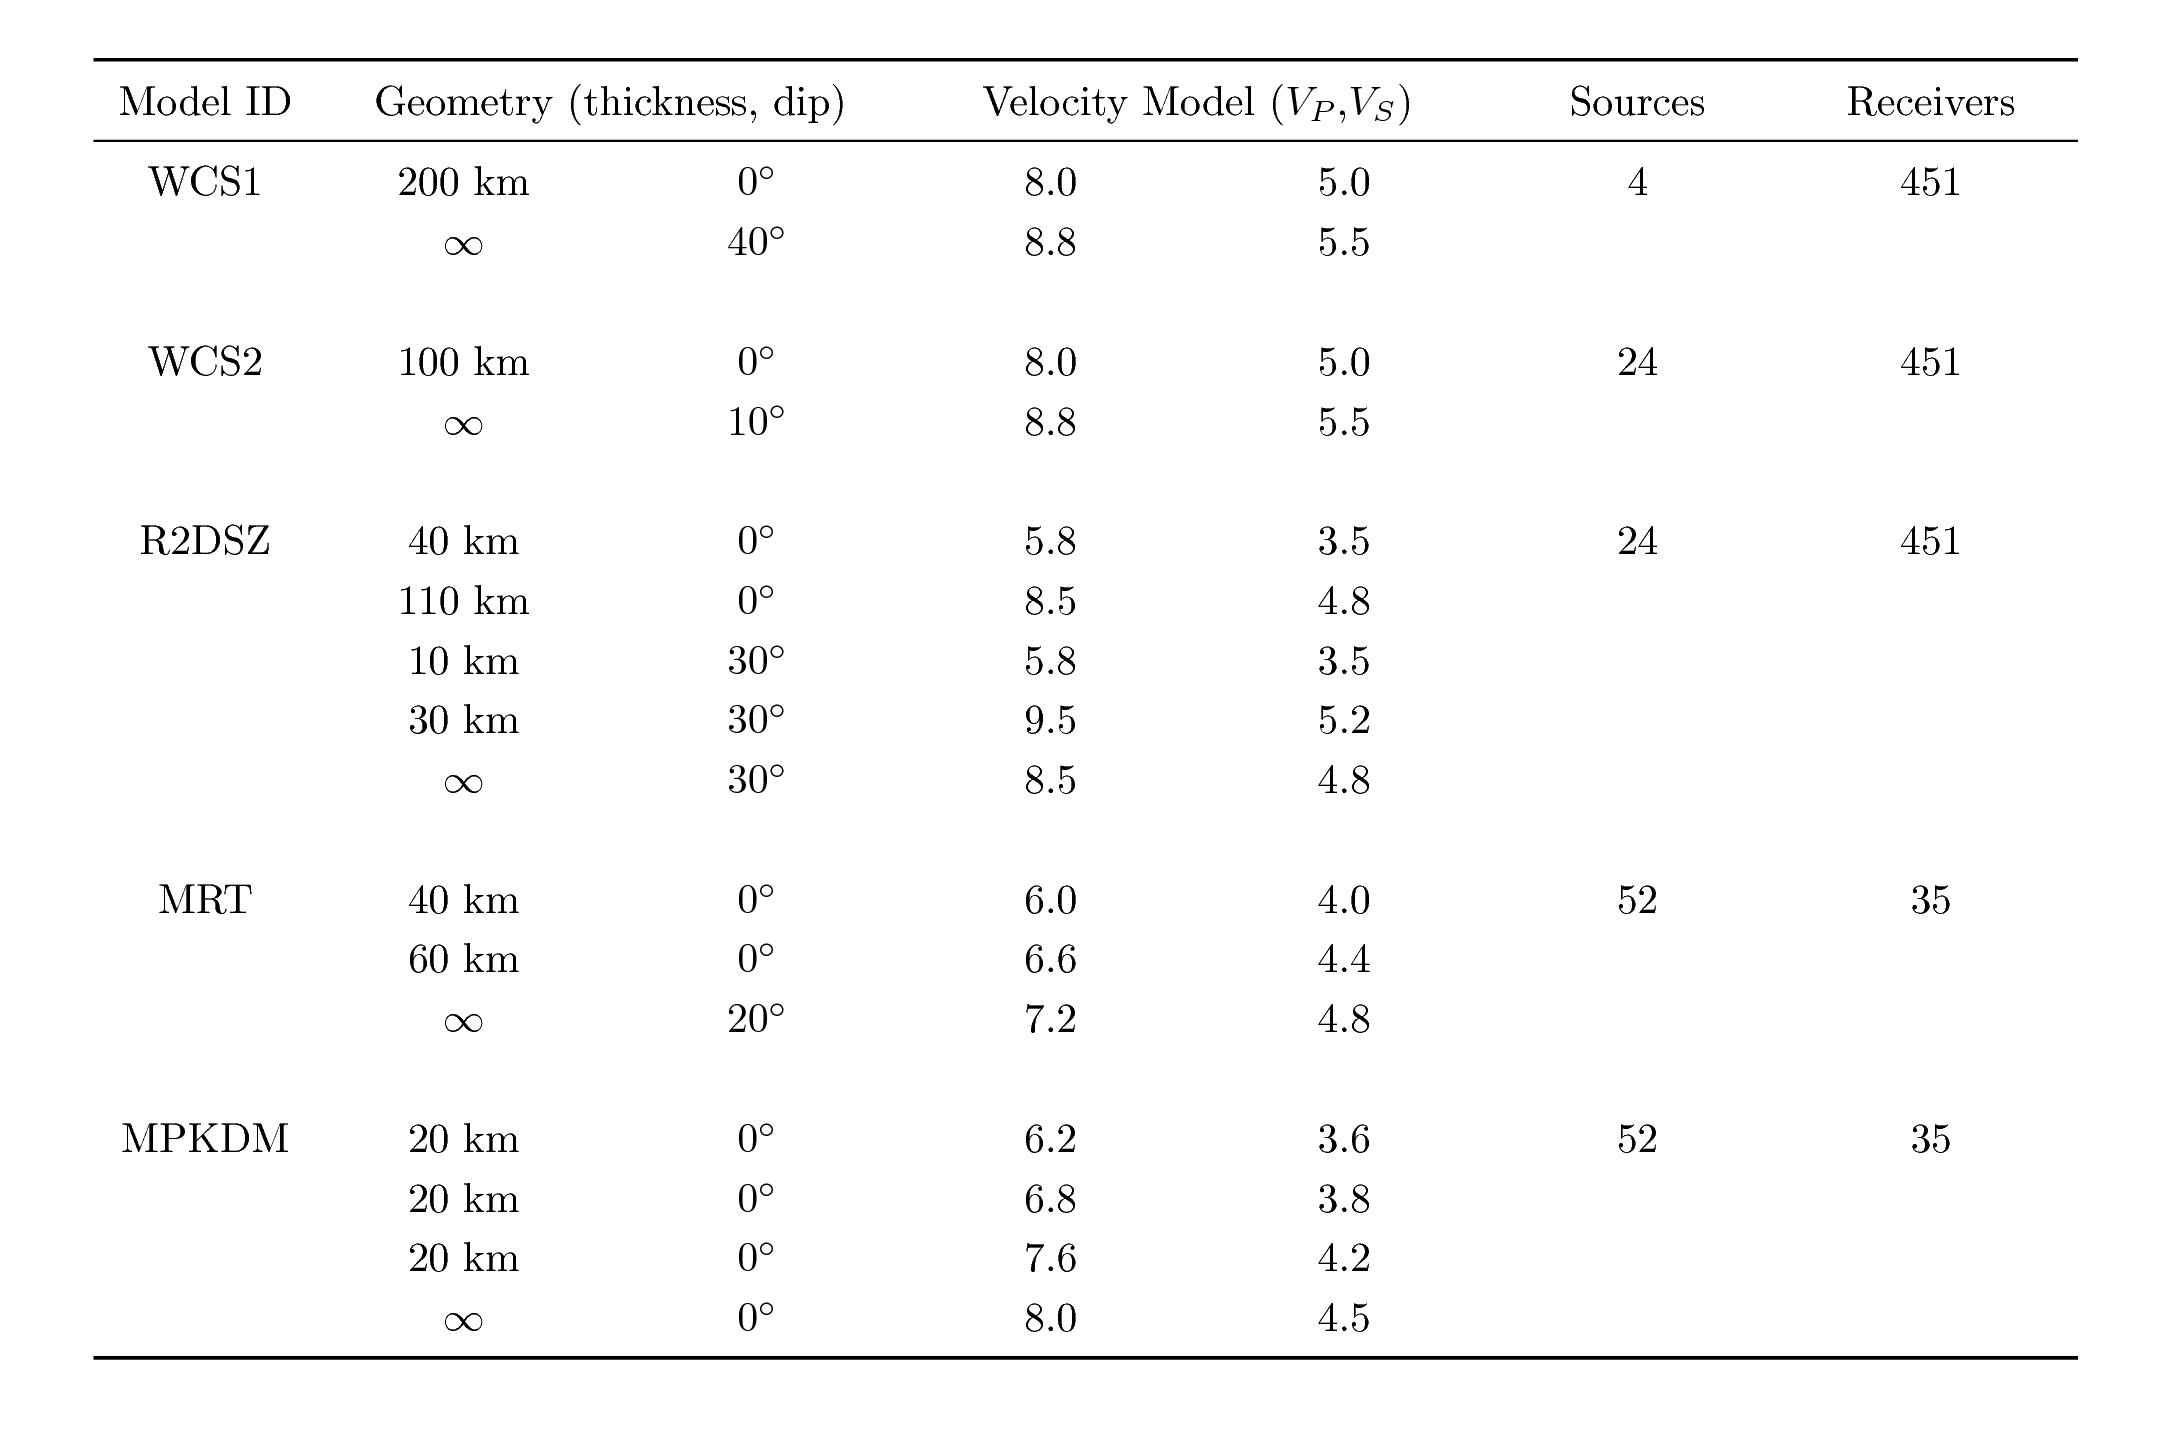
\includegraphics[trim= 0 0 0 0,clip,page=1,scale=.22]
                {../figs/finalfigs/ff13_3.png}
%                {../figs/finalfigs/ft1_2.png}
\caption{
Synthetic models and setups.
Dip corresponds to the upper interface of the layer. 
$V_P$ and $V_S$ are given in $km \cdot s^{-1}$ and $\infty$ corresponds to the semi-infinite layer at the bottom of the model. 
Thickness is taken at the center of the model and corrected for dip.
}
\end{table*}
%-----------------------------------------%
%     T     A     B     L     E     S     %
%-----------------------------------------%

%  -  -  -  -  -
% Subsubsection
%  -  -  -  -  -
\subsubsection{Synthetic models}

%%%\citet{cheng_gji_16} \hl{showed that taking the physics of the scattering into account is necessary to retrieve correct information from all RF data in subduction regions as polarities and amplitudes can largely vary with source-receiver geometry.
%%%Moreover, these variations have different characteristics on all three components of the recorded wavefield.}
%%%\citet{tone_epsl_08} \hl{proved that by exploiting radial and transverse RFs together a clearer understanding of dipping interfaces can be gained.
\hl{Here we conduct a series of synthetic tests on three synthetic models that we designed to show how including scattering patterns, three component RFs and free-surface multiples in the migration improves the final images.
They are described in table1 and hereafter.
The experimental setting for the third synthetic scenario (R2DSZ) is shown in fig4.}

The first synthetic model WCS1 represents a worst case scenario with respect to strong amplitude artifacts.
In particular, the polarity reversals in the data, that arrise from steep arrivals on dipping discontinuities, need to be adressed to correctly interpret the data \citep{cheng_gji_16}.
The first model WCS1 \hl{comprises} 2 layers separated by an interface with contrasts of 10$\%$ in $\alpha$, $\beta$ and $\rho$ at a 40$^{\circ}$ dip.
It corresponds to the synthetic case shown in \citet{cheng_gji_16}, \hl{and we expand the study of this setting by migrations three component data.}

The second synthetic model WCS2 represents a worst case scenario regarding the influence of the free surface mutliples.
It has the same elastic contrasts and a 10$^{\circ}$ dip.
These two synthetic cases are implemented to demonstrate the importance of accounting for scattering patterns and free surface scattering modes when migrating three component RF data.

The third model R2DSZ \hl{comprises} 5 layers and represents an idealized 2D subduction zone.
The first layer is a 30 km thick over-riding crust.
The second layer is the over-riding mantle.
The third and fourth layers are the subducting crust and lithospheric mantle that form the subducting plate, with respective thickness of 10 and 30 km, and dipping at a 30$^{\circ}$ angle.
The last layer is the unperturbed mantle under the subducting plate.

%-----------------------------------------%
%     T     A     B     L     E     S     %
%-----------------------------------------%
\begin{table*}[t]
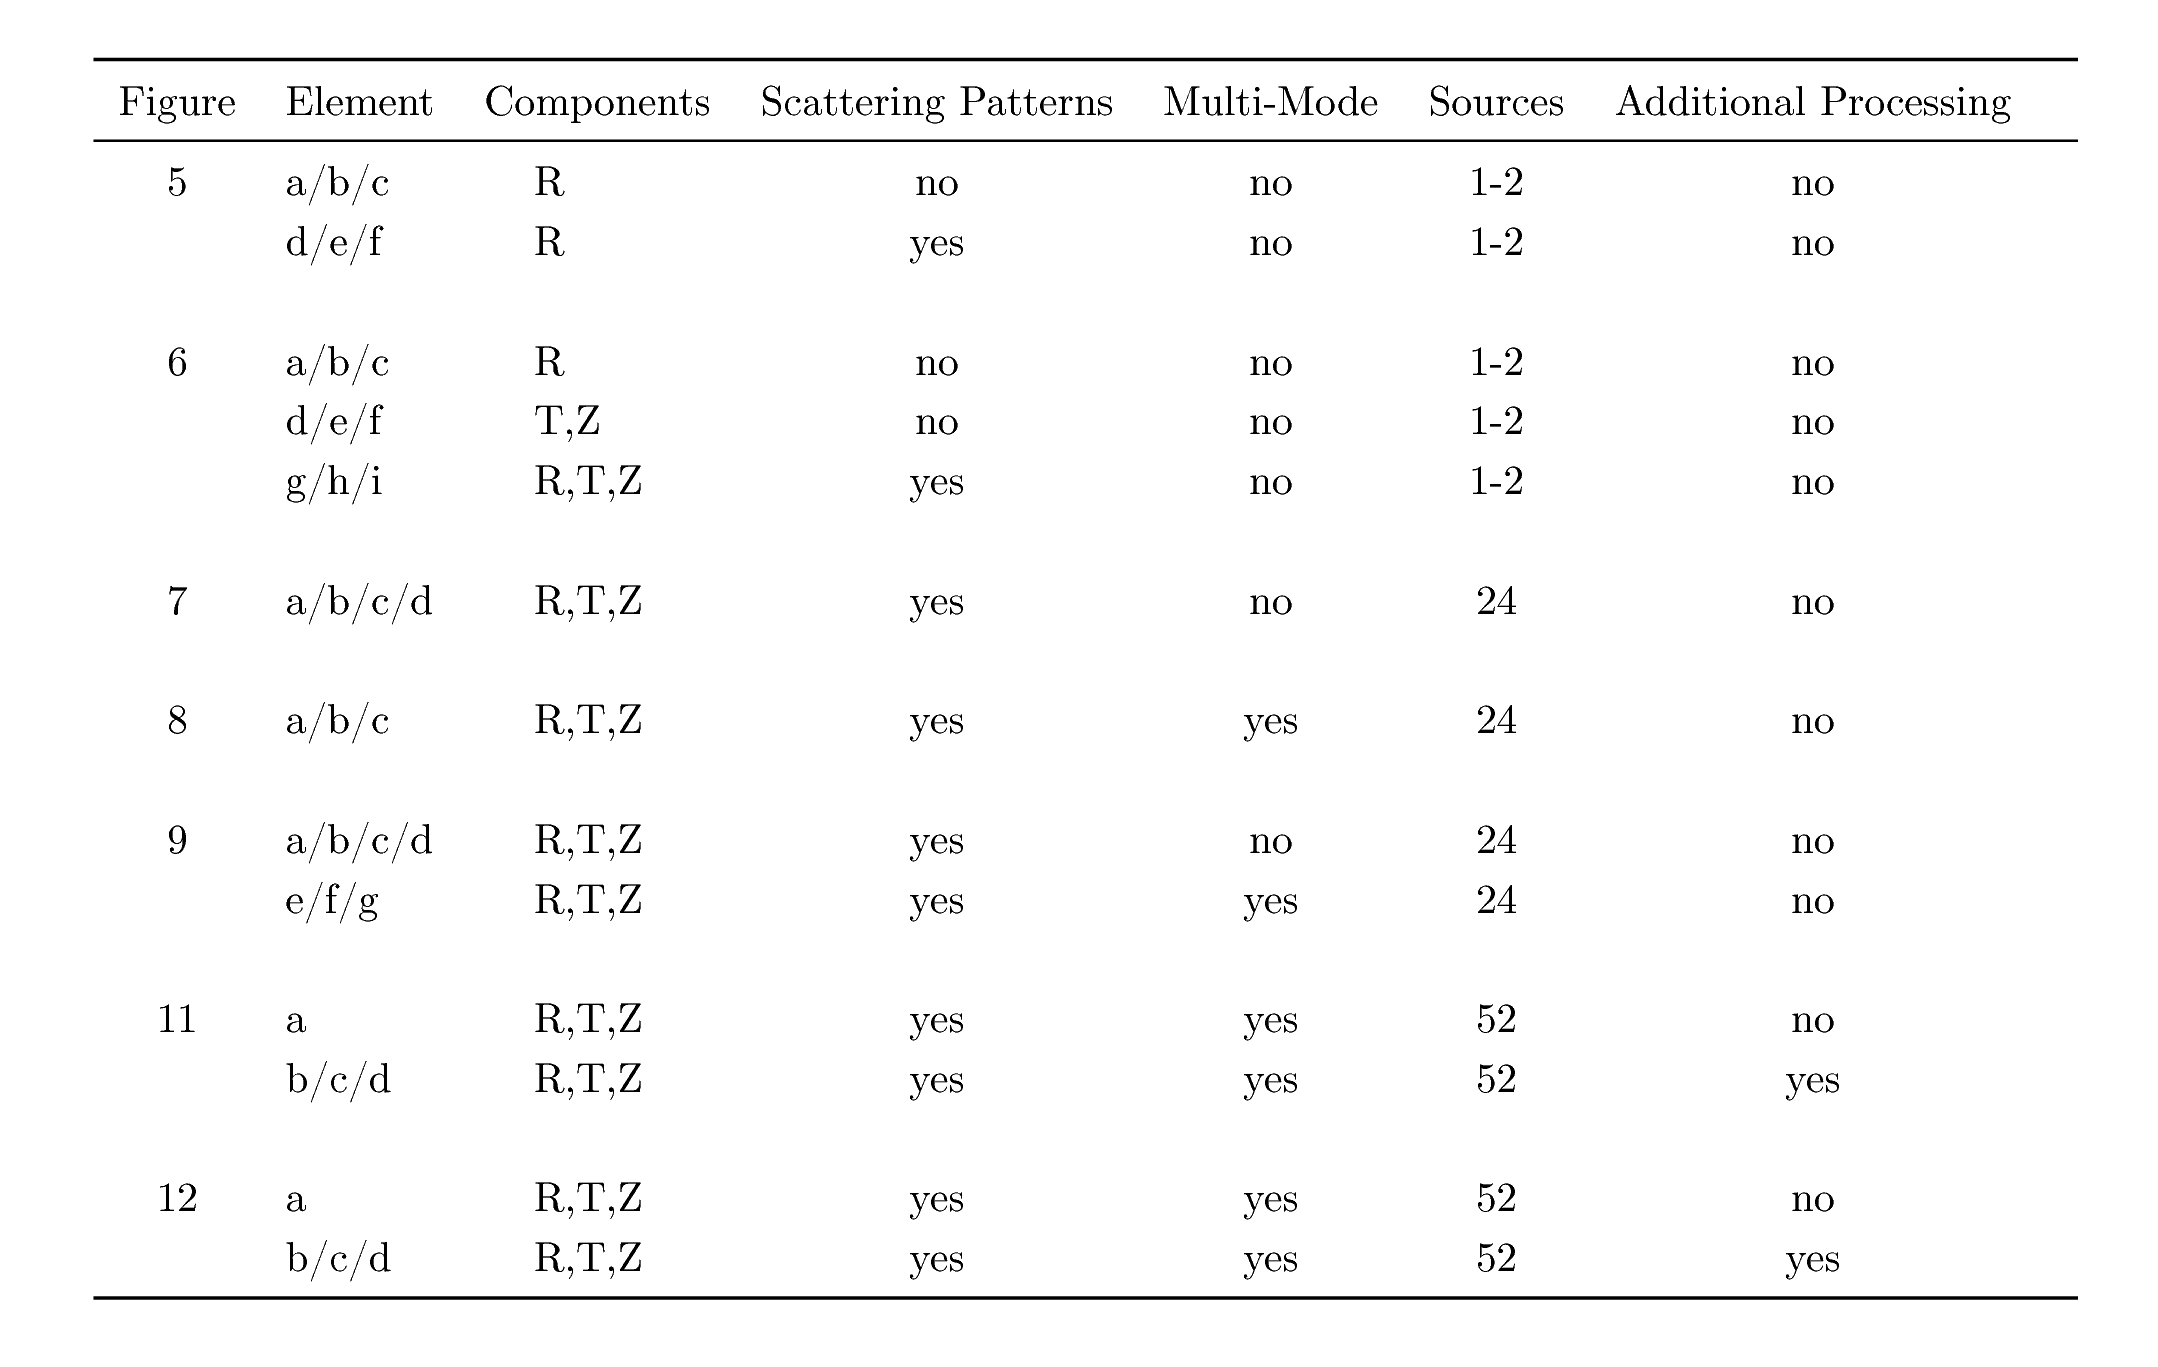
\includegraphics[trim= 0 0 0 0,clip,page=1,scale=.22]
                {../figs/finalfigs/ff14_3.png}
%                {../figs/finalfigs/ft3_2.png}
\caption{
Index of migrated sections with the effects taken into account for each.
Additional processing corresponds to the projection of the stations along the imaging line in the case of the MEDUSA experiment.
}
\end{table*}
%-----------------------------------------%
%     T     A     B     L     E     S     %
%-----------------------------------------%

%  -  -  -  -  -
% Subsubsection
%  -  -  -  -  -
\subsubsection{Synthetic setup}

In order to demonstrate that our migration method can be applied at continental scale, we decided to test it on a synthetic array that spans 100 by 400 km (fig4).
The array \hl{comprises} 11x41 stations that are regularly spaced, with station spacing of just above 10 km.
The sources are regularly spaced in back azimuth\hl{, i.e. every 90$^{\circ}$ for WCS1/WCS2 and every 15$^{\circ}$ for R2DSZ.
They are given a random epicentral distance from the center of the array between 30$^{\circ}$ and 90$^{\circ}$.
This simulates arrivals from a realistic range of} slownesses and back azimuths.
We acknowledge that this is an idealized geometry that rarely is available with field data as arrays usually have irregular shapes and sample an irregular distribution of back-azimuths.
We used up to 24 sources and created a total of up to 10824 synthetic waveforms for each synthetic velocity model.

For the \hl{models WCS1 and WCS2}, applying the successive imaging principles will help us demonstrate the \hl{improvements offered by three component RFs and correcting for scattering patterns.}
For the realistic 2D subduction \hl{(model R2DSZ), we expect this setup to image} the over-riding and subducting crust as a clear positive peak.
We also expect the method to \hl{resolve} both the crust and the LAB of the subducting slab.

%  -  -  -  -  -
% Subsubsection
%  -  -  -  -  -
\subsubsection{Synthetic waveforms}

The synthetic data are generated with a ray-based approach for modeling teleseimic body waves in dipping anisotropic structures \citep[Raysum software,][]{fred_gji_00}.
This \hl{approach} computes the arrival times and amplitudes of all converted and reflected \hl{(i.e., first-order free surface multiples)} phases in a layered geometry.
The advantage of this algorithm is that it is accurate and computationally efficient as it uses analytical formulae to compute the travel times, amplitudes and phase of the transmitted and scattered waves.

It can handle a large number of planar, homogeneous anisotropic layers with arbitrary strikes and dips.
However, the models cannot contain velocity or anisotropy gradients inside the layers and the layers themselves cannot intersect in regions \hl{that are traversed by rays}.
Because of these limitations, we could not simulate a \hl{laterally limited slow mantle wedge} in our idealized subduction zone model.
\hl{Since our simulations cannot reproduce fully 3D conditions}, we will refer to them as 2.5D synthetics hereafter.

Raysum outputs an ensemble of diracs convolved with a Gaussian source time function with a variable standard deviation, set to 3 seconds in our case.
We use this data directly as our “receiver functions”, without noise, as our source function is already a Gaussian.
%Our synthetic tests are performed without noise.

%  -  -  -  -  -
% Subsubsection
%  -  -  -  -  -
\subsubsection{Overall computational cost}

\hl{The Eikonal solver estimates the travel times of scattered waves through a cube of} 6$^{\circ}\times$6$^{\circ}$ in latitude and longitude and 500km in depth.
\hl{Our migration is perfomed in a cube of} 5$^{\circ}\times$5$^{\circ}$ by 450km depth to account for potential border effects in travel-time calculations.
The computations and migrations for all the synthetic cases were carried out on a single core \hl{of an Intel Xeon E5-2650 v2 Octocore processor}.
The Raysum and analytical signal computation take under two minutes to run.
\hl{The exact number of sources and receivers used for every model, for synthetic and field data, are detailed in table2.}
Running FM3D for 24 sources and 451 receivers takes three hours with a voxel size of 5$\times$5$\times$5km, on average.
The migration of the 10824 RF with the multi-mode algorithm also takes three hours to run.
\hl{The smaller experiments on the models WCS1 and WCS2 take 15 minutes and one hour respectively to run all steps.}

%-----------------------------------------%
%     F     I     G     U     R     E     %
%-----------------------------------------%
\begin{figure*}[t]
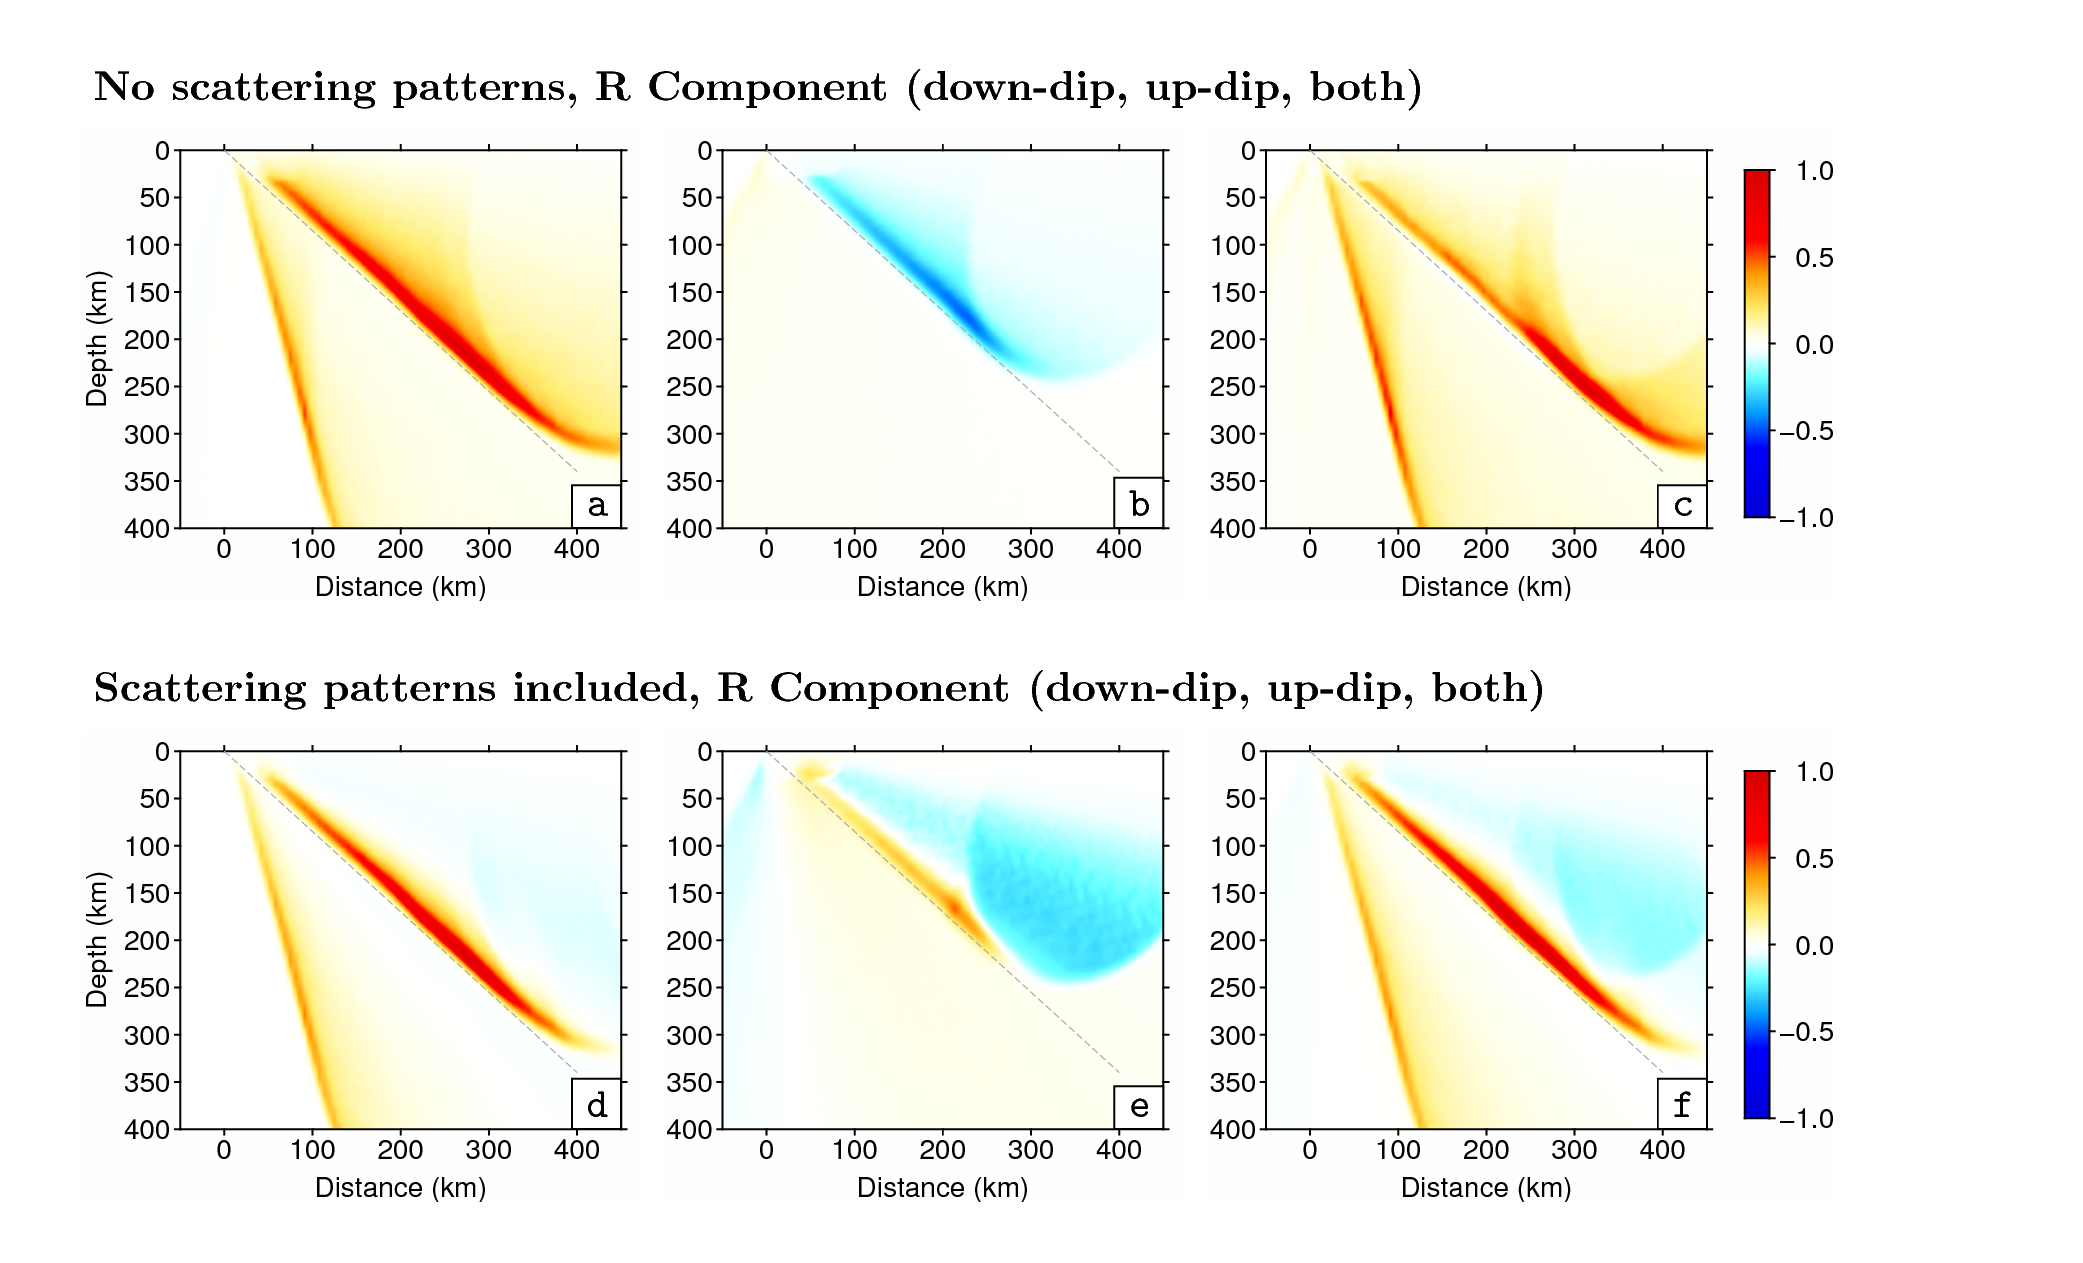
\includegraphics[trim= 0 0 0 0,clip,page=1,scale=.22]
                {../figs/finalfigs/ff5_3.png}
\caption{
Influence of the Scattering Patterns.
PS migration of the radial component of the RF for a 2D model with a single interface at 40$^{\circ}$ dip and 10\% $\delta V_P$, $\delta V_S$ and $\delta \rho$ perturbations. 
(a) and (d) correspond to a down-dip source coming from the right-handside, (b) and (e) to an up-dip source coming from the left-handside, (c) and (f) correspond to the stacks of (a+b) and (d+e) respectively. 
(a) to (c) are migrated without the scattering patterns and show inconsistency in the migrated polarity. 
(d) to (f) are migrated with the effects of scattering patterns taken into account and show consistent polarity, which improves the stacked image.
}
\end{figure*}
%-----------------------------------------%
%     F     I     G     U     R     E     %
%-----------------------------------------%

% - - - - - -
% Subsection
% - - - - - -
\subsection{Imaging potential of scattering patterns and three-component migration}

As shown in \citet{cheng_gji_16}, the scattering patterns are important not only to retrieve relative amplitude between the various phases but also to account for correct polarities on dipping reflectors.
\hl{In this section, we illustrate this point by applying the method} to the synthetic case described as WCS1 in table1, with a single 40$^{\circ}$ dipping interface.
Results are shown in \hl{fig5 and fig6.}

The \hl{migrated images} for the PS mode of two sources coming from opposite sides of the structure, both in the imaging plane, are shown in fig5.
\hl{The wavefield for the first source (left column) comes from a down-dip directions, which is to the right in this geometry.
The wavefield for the second source (middle column) comes from an up-dip direction, which is to the left in this geometry.
The results for two sources that were rotated 90$^{\circ}$ compared to the previous ones, which puts them in the strike parallel plane, are shown in fig6.
The wavefield for the first source (left column) comes from the reader's perspective into the figure and the wavefield for the second source (middle column) comes from the opposite direction, facing the reader.}
We illustrate our method with single-source migrations \hl{by introducing the various elements described in section 2 one by one.}
Table2 describes which \hl{elements of the imaging principle are} taken into account in every figure.

\hl{We shall now describe the each pannel of figs5 and 6.}
In Fig5 we migrate the radial component of the PS mode in the simple 2D model WCS1 to show the effect of applying the scattering pattern corrections.
The images from fig5a to 5c (top row) are migrated without taking the scattering patterns into account.
In fig5a (source on the right-hand side, first column) the migration algorithm focuses most of the energy on the discontinuity (black line).
However, the free surface back-scattered phases \hl{leak into the image and introduce} spurious structures with higher dip values and alternating signs.
A \hl{significant amount of scattered} energy has been smeared in the migrated image and is visible above the discontinuity.
The image in fig5b shows that for a source on the opposite side (second column) the migration also focusses the energy on the discontinuity at the correct depths but the polarity reversal has not been accounted for and the sign of the migrated scattering potential is negative.
Notice also that this image contains less energy from the multiples as this particular geometry generates less scattering overall on the radial component of the RF.
Fig5c shows that the image generated by linearly stacking over both sources (third column) is largely dominated by the wavefield coming from the down-dip direction and that the two sources interfere destructively where they are supposed to stack up.

If we apply the amplitude and polarity corrections given by scattering patterns and redo the same migration, we can see on fig5d and fig5e (bottom row) that the sign of the scattering potential of the imaged structures are now coherent for the two sources.
We also note that the image where the wavefield is coming from the down-dip direction (source on the right-hand side, first column) is significantly clearer as the positive and negative parts of the scattering pattern correction ellipse globally cancel out far away from the scattering interface.
The results in fig5f show that, even if the sum over the two sources is still dominated by the wavefield coming from the down-dip direction, this time the two images interfere coherently where they are expected to.
\hl{This proves that taking scattering physics into account greatly improves the imaging:} we migrate the correct polarities each time and the images stack constructively.
We eliminate the polarity problem for large dip angles and can automatically assimilate data from all slownesses.

%-----------------------------------------%
%     F     I     G     U     R     E     %
%-----------------------------------------%
\begin{figure*}[t]
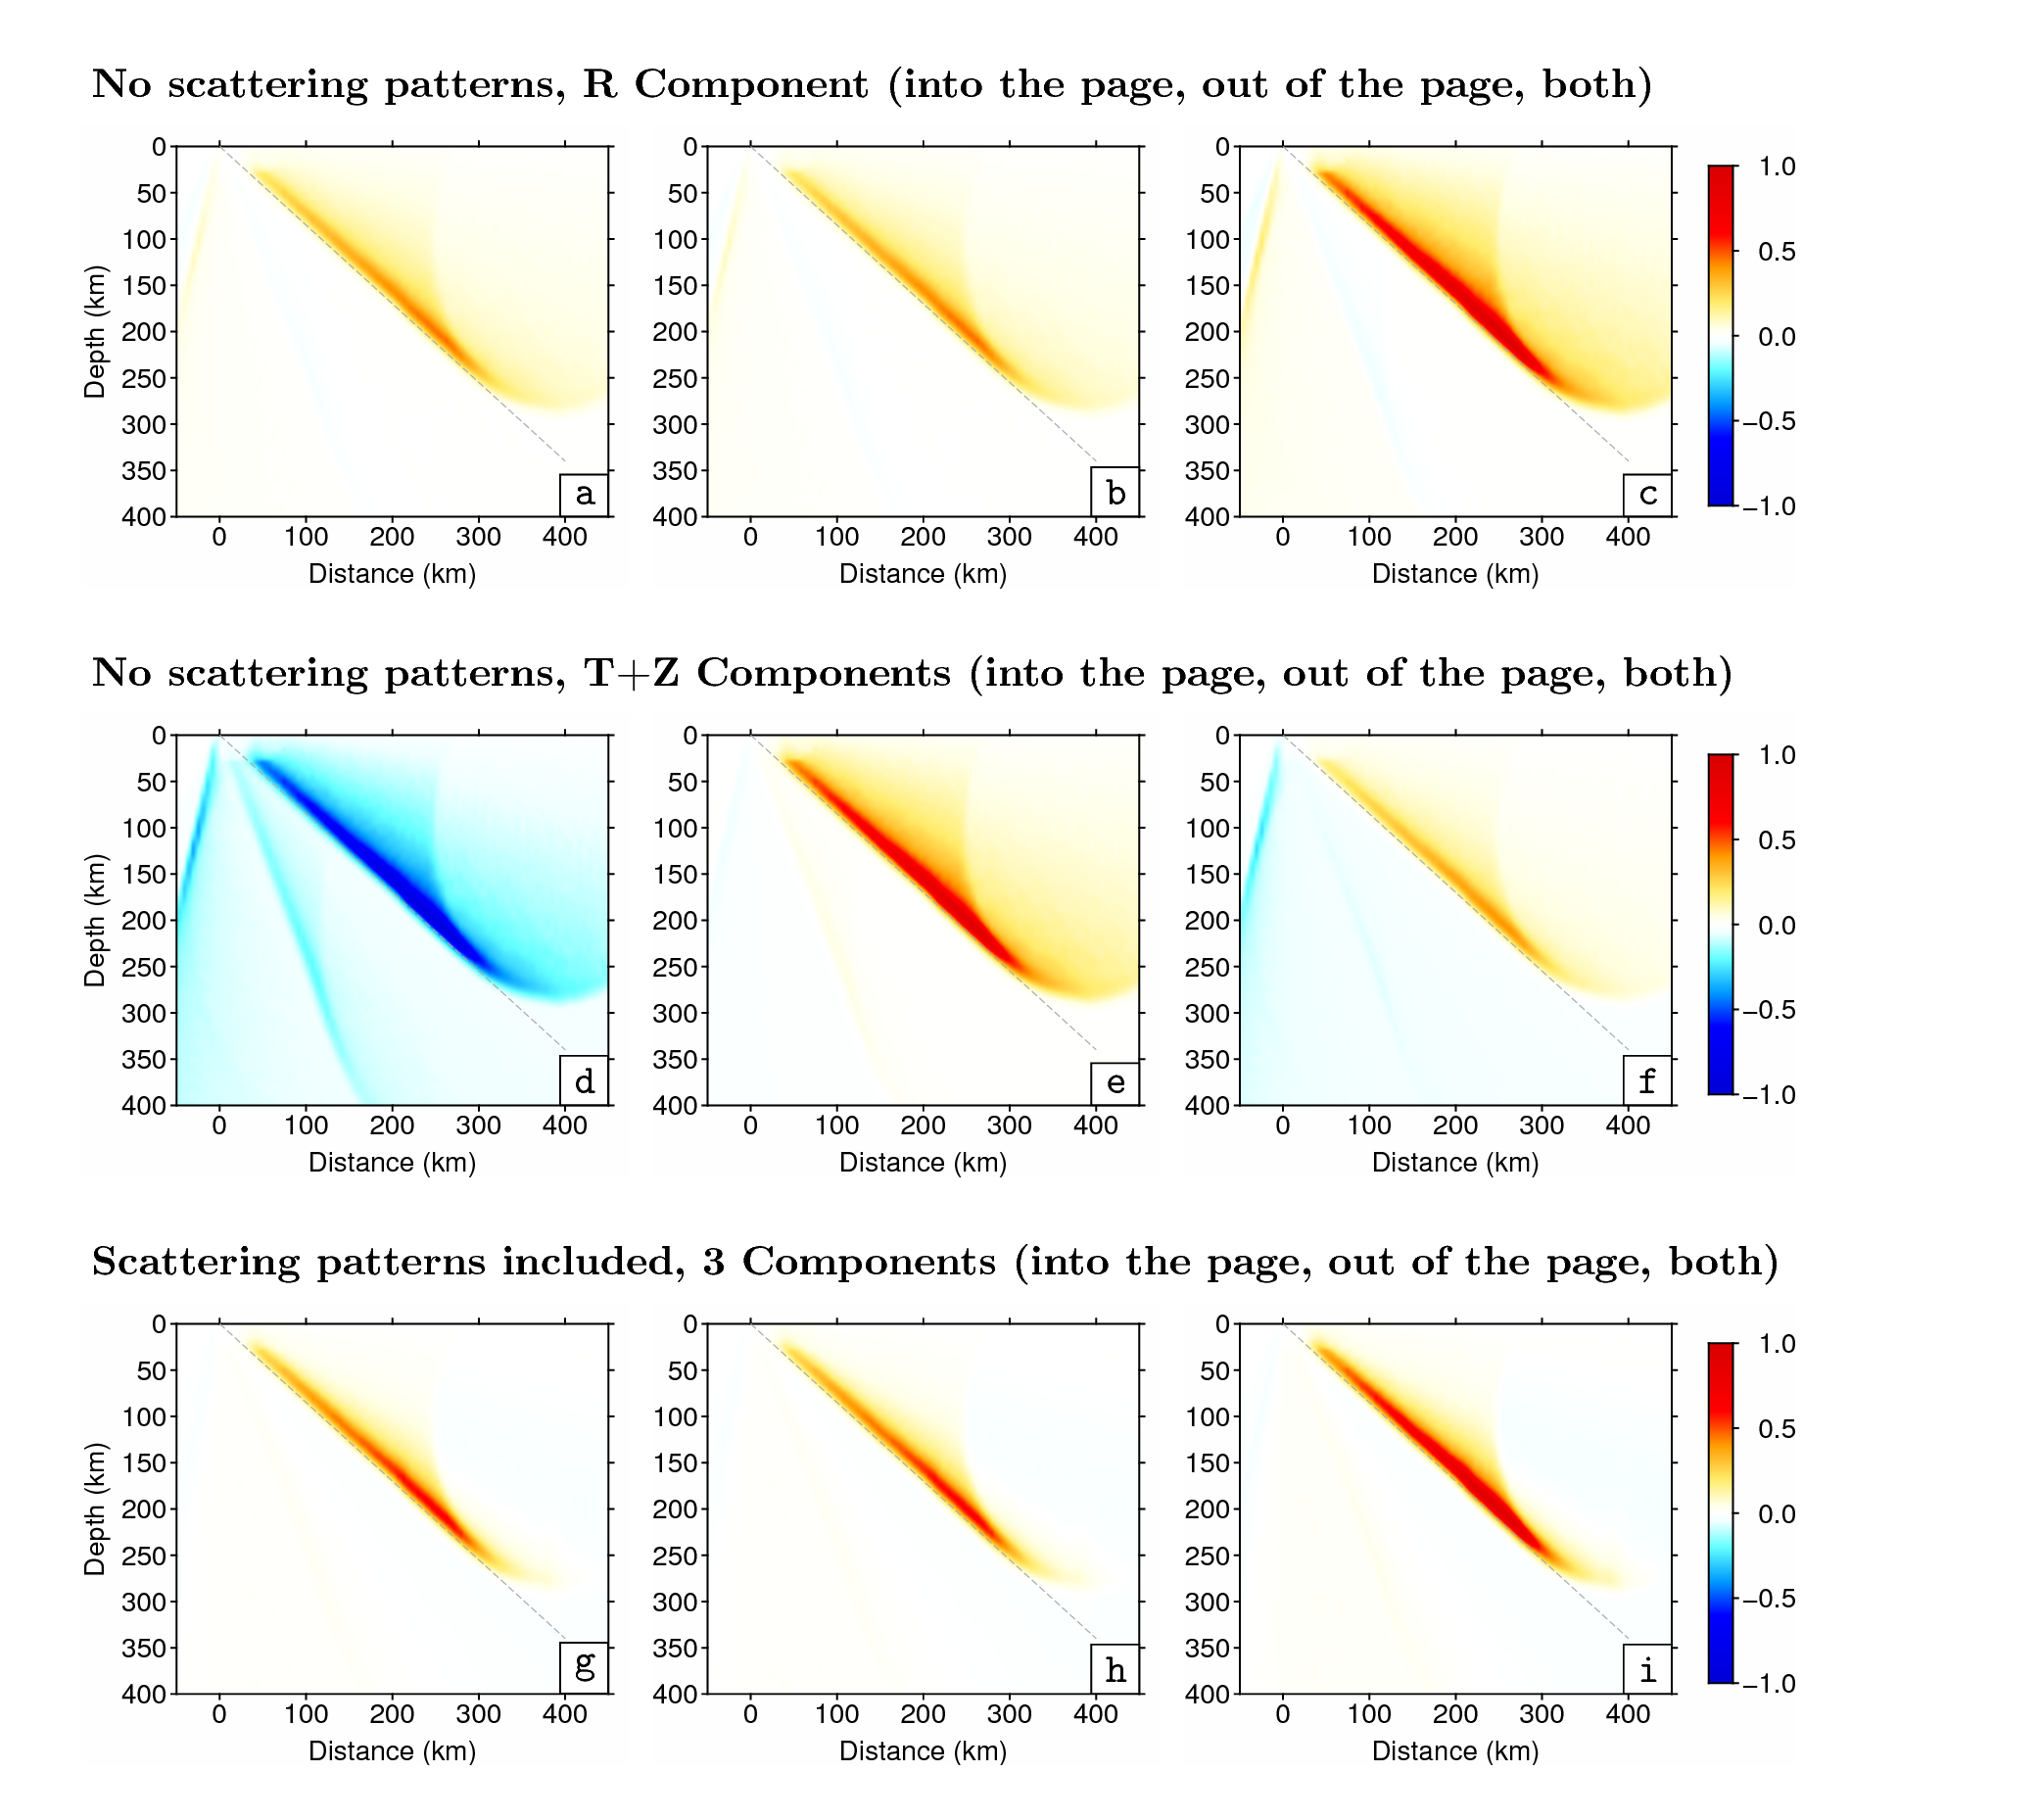
\includegraphics[trim= 0 0 0 0,clip,page=1,scale=.22]
                {../figs/finalfigs/ff6_3.png}
\caption{
Influence of the three component migration.
PS migration for a 2D model with a single interface at 40$^{\circ}$ dip and 10\% $\delta V_P$, $\delta V_S$ and $\delta \rho$ perturbations. 
(a), (d) and (g) correspond to an along-strike source coming from the readers perspective, (b), (e) and (h) to an along-strike source coming from the other direction, (c), (f) and (i) correspond to the stacks of (a+b), (d+e) and (g+h) respectively. 
(a) to (c) are the radial components of the RFs migrated without the scattering patterns and show cohenrent but relatively low amplitudes compared to figure 5a. 
(d) to (f) are transverse and vertical components of the RFs migrated without the scattering patterns and show higher energy content but inconsistent polarities. 
In (g) to (i), the three components of the RFs migrated with the effects of the scattering patterns taken into account.
}
\end{figure*}
%-----------------------------------------%
%     F     I     G     U     R     E     %
%-----------------------------------------%

The benefit of migrating the 3 components of the RF for large dips for oblique, along-strike arrivals in the WCS1 scenario is shown in fig6.
We show that there is \hl{much} complementary information to be gained from 3 components migration, \hl{provided} that polarity reversals are properly accounted for.
Similarly to fig5, we migrate the PS mode for the same simple 2D model.
The results in fig6a to 6c (top row) show the migrated images of the radial component for two sources placed symmetrically on one side (into the page, first column) and the other (out of the page, second column) of the dipping structure.
It shows identical images for the two sources which is expected.
The signs of the discontinuities are correct in both images for the PS mode but we also see a lot of energy from the PpS and PsS multiples at higher dip angles.
The summed image (third column) in fig6c shows the same attributes.
However, the maximum absolute amplitude in this image is lower than in fig5a.
When migrating the transverse and vertical components of the RF in fig6d and 6e (middle row), the maximum amplitude is higher but \hl{there are} polarity issues.
Moreover, the images are not identical anymore because the transverse component is defined in opposite directions for both sources.
Therefore we can see in fig6f that the stack of the two previous images does not give a satisfactory result. %, as we image mostly artifacts.
By applying the scattering patterns on the three components, we solve the problem in fig6g to 6i (bottom row).
This time, by migrating the three components of the RF with their respective scattering weights, we find identical images again, which is what we expect after the correction, and the amplitude in the stacked images are on the same order of magnitude as their counterparts in fig5.
\hl{Here we showed the importance of the scattering patterns when migrating three component data.
Moreover,} integrating the three components of the RF into the imaging principle allows us to coherently retrieve the information about scattering for arbitrarily dipping discontinuities from all back-azimuths.

%-----------------------------------------%
%     F     I     G     U     R     E     %
%-----------------------------------------%
\begin{figure*}[t]
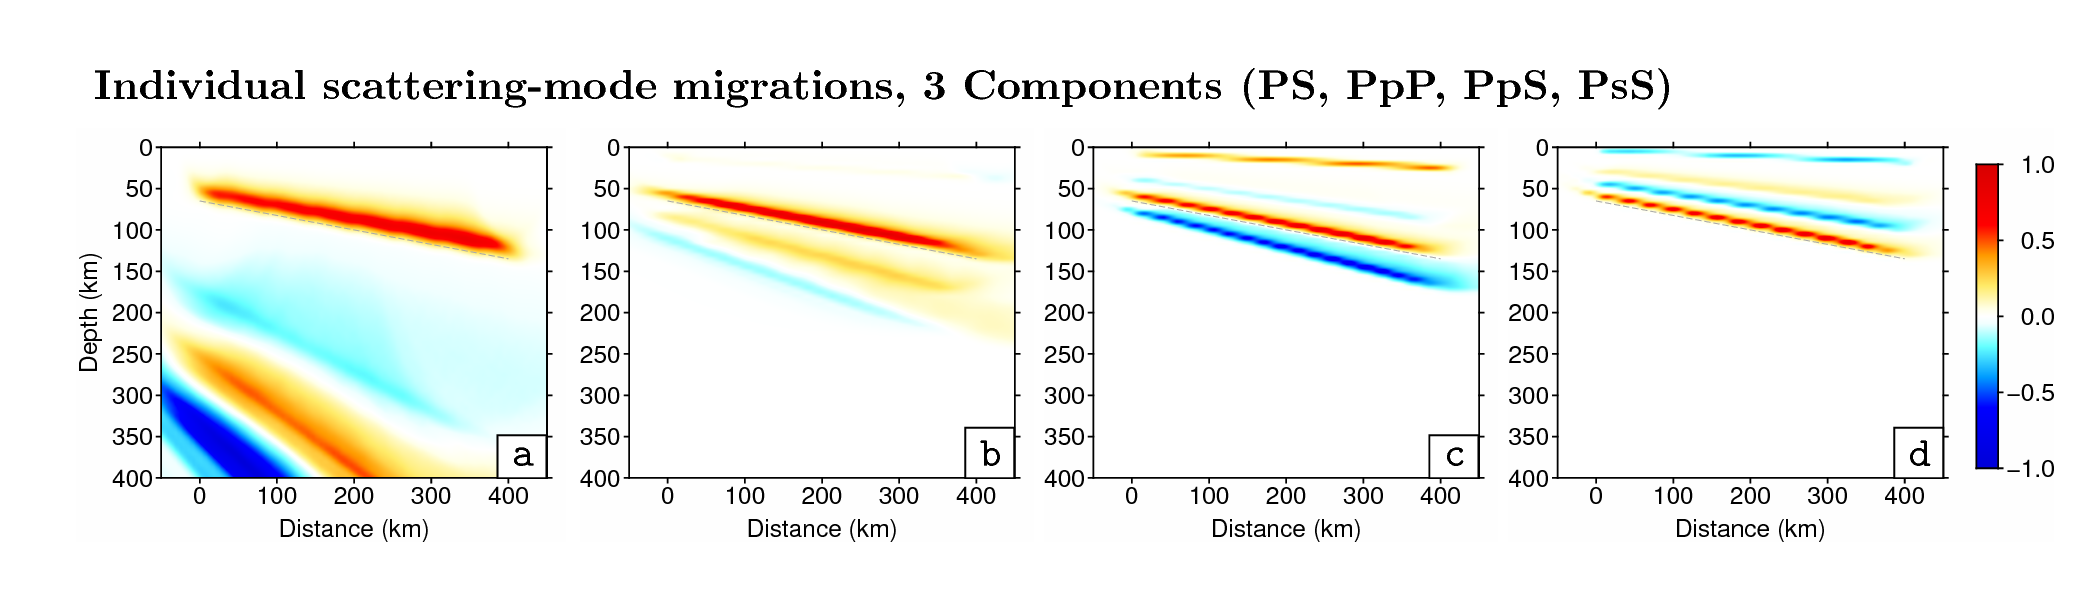
\includegraphics[trim= 0 0 0 0,clip,page=1,scale=.22]
                {../figs/finalfigs/ff7_3.png}
\caption{
Single-mode migrations of three components RF for a 2D model with a single interface at 10$^{\circ}$ dip and 10\% $\delta V_P$, $\delta V_S$ and $\delta \rho$ perturbations. 
(a) is the PS, (b) the PpP, (c) the PpS and (d) the PsS migrations (cf. text). 
24 sources regularly spaced in back-azimuth and with 30$^{\circ}$ to 90$^{\circ}$ of epicentral distance were used in the migrations. 
The four image recover the structure with the correct polarity but are affected by the other modes.
The spurious migrations are at different locations in each migration.
}
\end{figure*}
%-----------------------------------------%
%     F     I     G     U     R     E     %
%-----------------------------------------%

% - - - - - -
% Subsection
% - - - - - -
\subsection{Multi-mode migration}

As seen in fig5 and fig6, free surface multiples are clearly visible in the PS migration \hl{even for very simple settings.
They are easily distinguishable in the PS migrated image for this particular model but their interpretation become increasingly more difficult with the complexity of the setting.
Here we will show how migrating not only the four first-order scattering modes independently but also jointly we can mitigate the influence of the free surface multiples in the iterpretations of migrated images.}

Since free surface multiples tend to be stronger and more difficult to interpret correctly in sub-horizontal settings, we choose a model with a 10$^{\circ}$ dipping interface, and thus placed ourselves in a worst case scenario regarding the free surface multiples \citep{cheng_grl_17}.
\hl{In this simulation} we use 24 sources to cover all possible back-azimuth and incidence angles.
The results in fig7 show the migrations for the 4 \hl{individual scattering modes} for the scenario WCS2 described in table1, which has one interface at a 10$^{\circ}$ dip.

The results for the PS migration with the three components is shown in fig7a.
The black line shows the only feature that is present in the synthetic model.
We can see a coherent signal that lines up with \hl{the structure}, but also \hl{three spurious features associated with multiples: (1) a negative feature at approximately 150km to 300km depth that corresponds to the PpP multiple; (2) a positive feature at 250km to 400km depth that corresponds to the PpS multiple; and (3) a negative feature between 300km and 400km depth that corresponds to the PsS multiple.}

We perform the 3 migrations for the free surface multiples \hl{and the resulting images} can be seen on fig7b (PpP), fig7c (PpS) and fig7d (PsS).
We find that the free surface multiples in the synthetic waveforms are correctly migrated in their respective images.
However, in each image, three out of the four modes are \hl{still visible and} wrongly migrated. 
They appear at different depths, and \hl{produce spurious} structures with different dip angles.
\hl{Specifically}, phases slower than the currently migrated mode are mapped below the true scattering feature (e.g. in fig7a), and phases faster than the currently migrated mode are placed above the scattering feature (e.g. in fig7d).
On these four migrated images, there is overall more spurious features than true features, but their locations are not coherent across the four \hl{single scattering mode} migrations.
\hl{These four images allow us to visually discriminate between real features, that have coherent amplitude across all 4 images, and the spurious features, that do not corellate on the different single scattering-mode images.}

Because the time delays are more compressed in the multiple modes, they have a higher spatial resolution than the direct PS conversion mode, especially for the S scattered waves \citep{rond_sgeo_09}.
This is due to the fact that a ray covers a single unit distance (upgoing) between two consecutive points in depth for the PS mode and two (downgoing and upgoing) when we migrate a multiple.
%However, because the P-wave inherently has a wavelength that is half that of the corresponding S wave, the effect discussed before is balanced for the PpP multiple \citep{rond_sgeo_09}.

\hl{Here we showed that we are able to migrate the free surface multiples at their correct polarities and positions in depths using the scattering patterns and their respective travel times computed with FM3D.
These waves provide complementary images to the PS migration, and we will now show that we can extract the coherent information from all the scattering modes using different stacking schemes.
%We can mitigate the effect of spurious energy in the PS migration by migrating it together with the other modes, where the spurious energy focuses on different isochrons.
Because the actual features are always focused at the same depth across all single scattering-mode images, they will sum up positively during the multi-mode migration.}

%-----------------------------------------%
%     F     I     G     U     R     E     %
%-----------------------------------------%
\begin{figure*}[t]
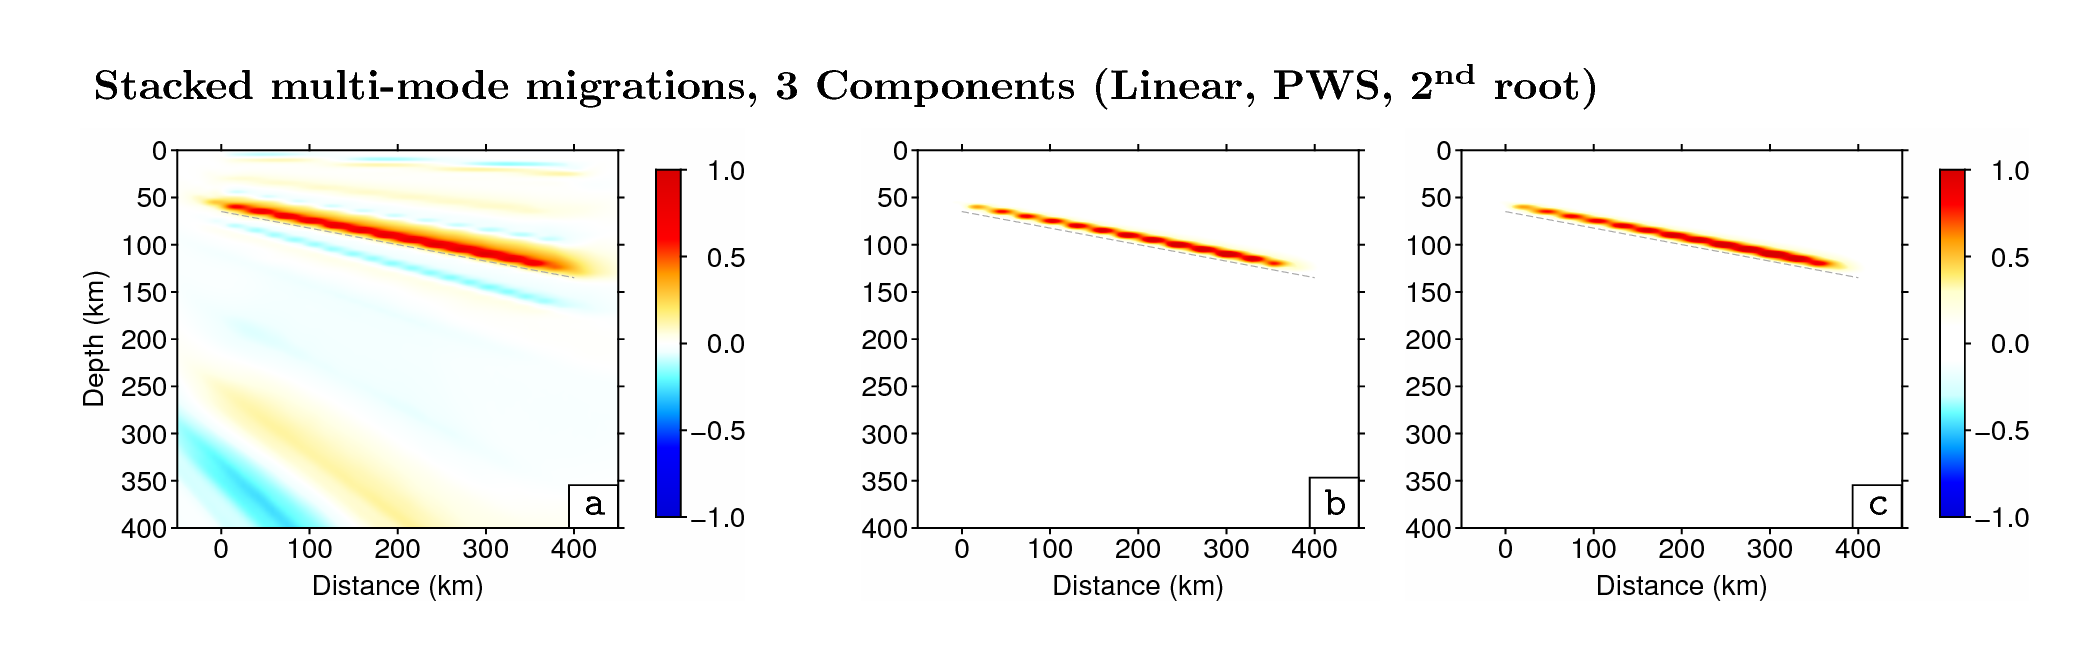
\includegraphics[trim= 0 0 0 0,clip,page=1,scale=.22]
                {../figs/finalfigs/ff8_3.png}
\caption{
Multi-Mode migrations for a 2D model with a single interface at 10$^{\circ}$ dip and 10\% $\delta V_P$, $\delta V_S$ and $\delta \rho$ perturbations.
(a) Linear, (b) phase-weighted and (c) 2nd root stacks for the multi-mode migration of the 3 component RFs with scattering patterns for 24 sources coming from all azimuths from 30$^{\circ}$ to 90$^{\circ}$ of epicentral distance.
}
\end{figure*}
%-----------------------------------------%
%     F     I     G     U     R     E     %
%-----------------------------------------%

% - - - - - -
% Subsection
% - - - - - -
\subsection{Stacking methods}

To extract the coherent signals in the four \hl{single scattering-mode migrated images in fig7}, we implemented three different stacking methods.
\hl{As detailed in Section 2.7, we implement one stacking method with no coherence filter} (linear stacking, eq.\eqref{foc}) \hl{and two stacking methods that incorporate coherence filters: phase-weighted stacking} (phase filter, eq.\eqref{pws}) \hl{and 2\textsuperscript{nd} root stacking} (amplitude filter, eq.\eqref{2rs}).
\hl{The results are displayed in fig8.}

The first \hl{method we test is linear stacking} (eq.\eqref{foc}, fig8a), where we simply add the energy of the four modes during the migration with no extra measure of coherence.
\hl{Results show that} the dipping interface is better imaged than on fig7a.
We note that the energy from spurious features is drastically reduced, but that they do not completely disappear.
\hl{The three spurious streaks described in fig7a} are still present just under the actual discontinuity.
%The thickest one corresponds to the PpP mode migrated in the PS image.
%The two thinner ones correspond to the PpS mode migrated in the PpP image and to the PsS mode migrated in the PpS image.
We also see that there is more noise above the discontinuity than in fig7a.
%\hl{We note the negative streak at the bottom of the image, corresponding to the PsS mode migrated in the PS image, does not disappear in the linear stack, because the amplitude in other images is zero there.}
%\hl{This highlights that} if a given mode is predominant in the record, then its contribution will also \hl{be prodominant} the final image.
%\hl{In the opposite case,} if 
\hl{In this case,} the four modes have comparable amplitudes, and spurious features will be reduced to about one fourth of their amplitude on a given scattering mode migration.

\hl{The second method we test is phase-weighted stacking and corresponds to the imaging principle in eq.}\eqref{pws}.
\hl{The results are shown in fig8b.}
The resulting image exhibits fewer artifacts than with the linear stack, as most spurious signals do not have a coherent phase over the 4 modes.
The phase stack virtually acts as a filter applied to the linear amplitude stack, as the artifacts are at the same position in depth but their amplitude is \hl{even more reduced, representing less than 10\% of their single-mode values.}
%It also focuses the energy on the scattering discontinuity even more, and the borders of the discontinuity are thinner.

\hl{Finally, the last nethod we test is 2\textsuperscript{nd} root stacking and corresponds to the imaging principle in eq.}\eqref{2rs}.
\hl{The results are shown in fig8c.}
The image is very similar to fig8b and has all the artifacts reduced to less than 10\% of the actual discontinuity.
%The focus of the positive peak on the scattering discontinuity is the same as for the phase-weighted stack in fig8b.

We have shown that most artifacts can be eliminated by applying coherence filters based either on phase (phase-weighted stack) or amplitude (2\textsuperscript{nd} root stack) in simple synthetic cases.
We are now going to test these methods with a more complex synthetic model depicting an idealized subduction zone.

%-----------------------------------------%
%     F     I     G     U     R     E     %
%-----------------------------------------%
\begin{figure*}[t]
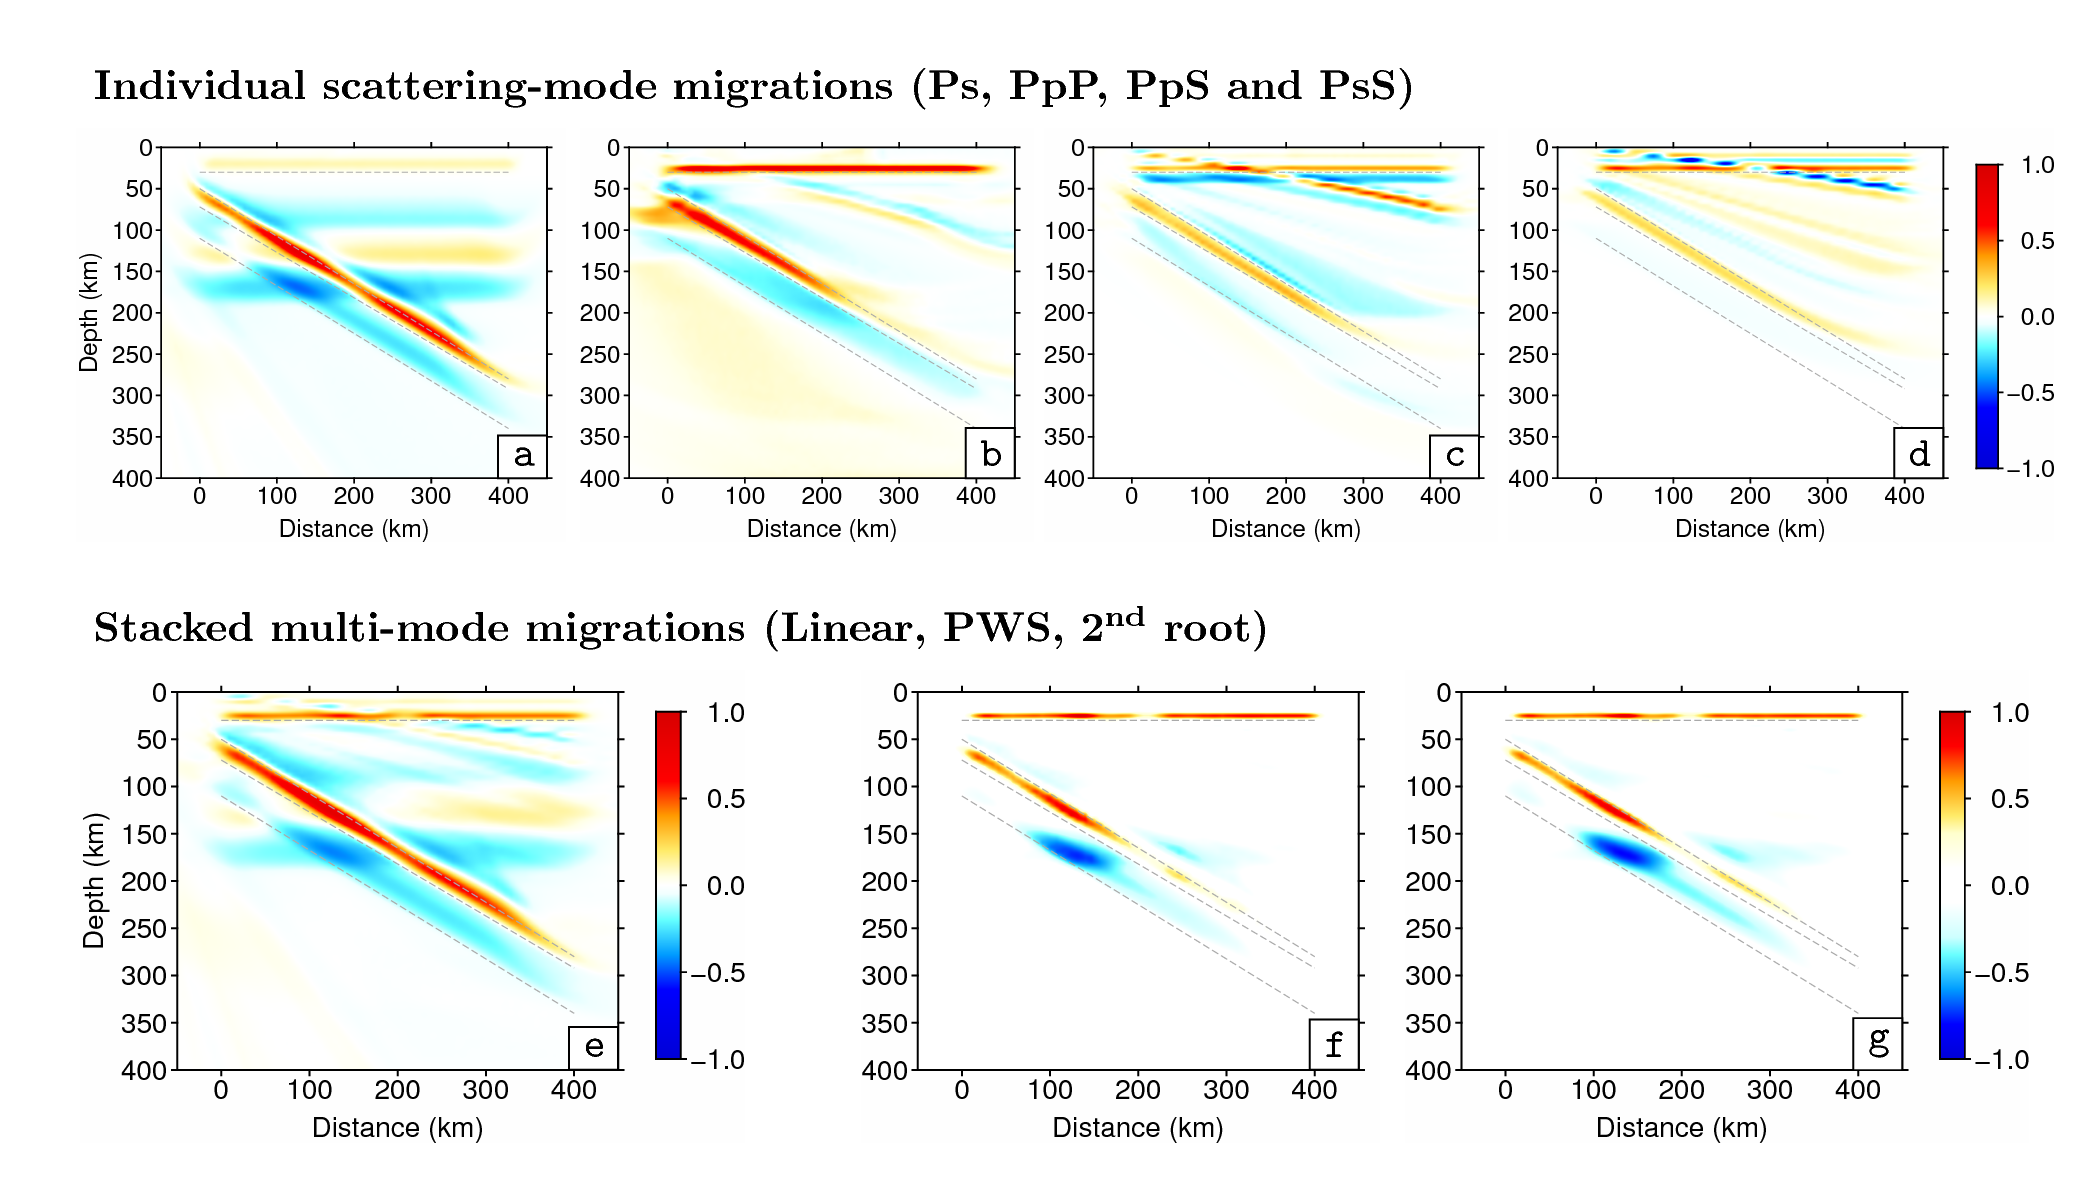
\includegraphics[trim= 0 0 0 0,clip,page=1,scale=.22]
                {../figs/finalfigs/ff9_3.png}
\caption{
Single scattering-mode and multi-mode migrations for the 2.5D Subduction Zone (R2DSZ, Table 1).
The upper 4 images (a=PS, b=PpP, c=PpS, d=PsS) are the 4 migrations for the 4 single-scattering modes (eq.\eqref{foc}). 
The lower 3 images correspond to the linear (e, eq.\eqref{lin}), phase-weighted (f, eq.\eqref{pws}) and 2\textsuperscript{nd} root (g, eq.\eqref{2rs}) stacked images.
}
\end{figure*}
%-----------------------------------------%
%     F     I     G     U     R     E     %
%-----------------------------------------%

% - - - - - -
% Subsection
% - - - - - -
\subsection{2.5D subduction zone}

Here we show how our imaging principle can be used to improve interpretations in realistic settings.
We designed a synthetic subduction zone, described as R2DSZ in table1, and analyse the migrated images obtained using eqs.\eqref{mod}, \eqref{foc}, \eqref{pws} and \eqref{2rs}.
In this case,we have 5 different layers with constant elastic properties and use a total of 24 sources equaly spaced in back-azimuth with random epicentral distance to the center of the array of 30 to 90$^{\circ}$.

\hl{The results for the 4 single mode migrations are shown in fig9a to 9d.
Fig9a shows the migration of the forward PS scattering mode.}
\hl{The single-mode migration} is able to resolve the Moho and the different dipping interfaces that constitute the oceanic lithosphere, but there are strong artifacts in the migrated image.
In the right part of the image, we show that for a simple 30 km deep Moho model, the free surface multiples can become predominant at around 100 km where one could interpret a spurious LAB.
Fig9 shows the back-scattered PpP migration.
The structure comes out more clearly because the PpP scattering mode is well isolated from the other phases as it \hl{is polarized mostly along the vertical component, whereas the S-waves from the other scattering modes are polarized mostly along} the horizontal components.
The results in fig9c and 9d show the back-scattered PpS and PsS migration respectively.
They exhibits both clear artifacts in the over-riding mantle wedge, that correspond to the spurious migration of the other three phases for the slab conversions, as well as clearly defined structure for the Moho and the subducting slab.
The higher resolution of the backs-cattered S modes are visible on these last two figure. %already, but as the streaks close to the Moho are very close to another, it is difficult to interpret structure on its own.
Overall, the images for free surface multiples’ migrations have less imaging power in the lower part of the image because phases reflected on the top of dipping interfaces at these depth are not recorded on the array and leave the imaged region.
The considered scattering modes are always migrated at the correct position in their respective images while the other modes are migrated at different locations. 

\hl{The results for the 3 different stacking methods are displaed in fig9e to 9g.}
Fig9e corresponds to the linear stack.
It represents a strong improvement over fig9a.
\hl{However, because the PS mode is dominating the final image, phases reflected at the continental Moho and migrated as PS transmissions are still visible.}
We also note that the free surface multiples for the dipping interfaces are not misplaced anymore. %and that the image is more focused at the actual scattering interfaces.
Fig9f corresponds to the phase-weighted stack that focuses the energy even more at the true location of discontinuities, especially in the upper part of the subducting slab.
There are still some visible artifacts but their amplitude is now one order of magnitude \hl{smaller than} the amplitude associated with the correctly migrated interfaces.
Finally fig9g corresponds to the 2\textsuperscript{nd} root stack.
%In this image, artifacts are not visible anymore.
%However, the signal from the Moho and the contact between the bottom of the slab and the oceanic asthenosphere have become smaller because they stack up less than the slab.
\hl{This image is very similar to the phase-weighted migration, and the slab is recovered down to 200 km depth.}
\hl{This proves that it is necessary to adopt a multi-mode migration strategy in order to avoid misinterpreting Moho multiples as a potential LAB.}

\hl{In this section, we showed that the imaging principles that we developed in section 2 are able to structure in both challenging and realistic settings.
We tested the method with worst case scenarios with respect to polarity artifacts (WCS1) and strong free surface multiples (WCS2), as well as with a synthetic 2D subduction zone (R2DSZ).}
The data can be automatically processed with the scattering patterns on three components.
This ensures maximum data coverage and allows for good focusing of the migrated energy along the scattering interfaces.
Now that we have shown how this works in detail on synthetic examples, we apply the imaging principles to field data from the MEDUSA array in the Hellenic subduction zone.
We show that we are able to retrieve the subsurface structure with fine details and find potential coherent seismic evidence for partial melting under Sousaki volcano.

%---------
% Section
%---------
\section{Application to field data and discussion}

%-----------------------------------------%
%     F     I     G     U     R     E     %
%-----------------------------------------%
\begin{figure*}[t]
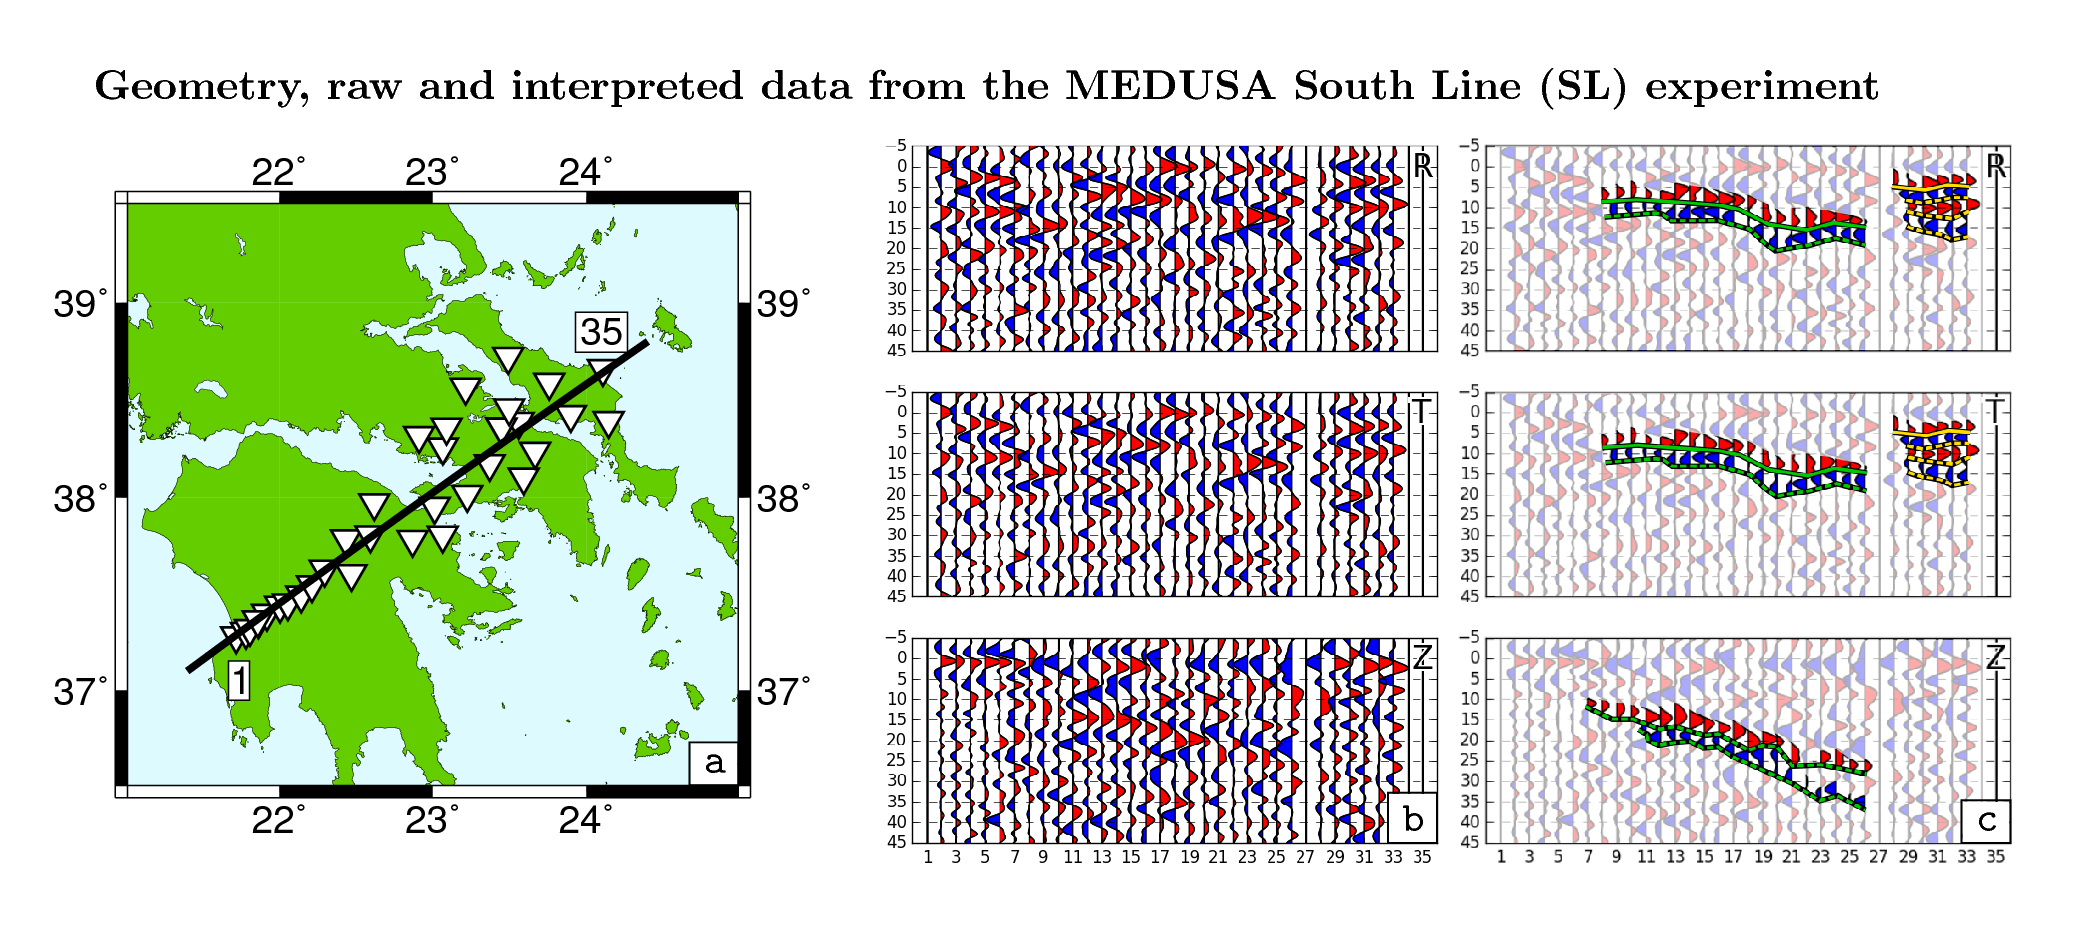
\includegraphics[trim= 0 0 0 0,clip,page=1,scale=.22]
                {../figs/finalfigs/ff10_3.png}
\caption{
Setup, raw and interpreted date from the MEDUSA experiment \citep{pear_jgr_12}. 
(a) corresponds to the array setup, with white triangles representing the stations position from 1 (south-western corner) to 35 (north-eastern corner) and the projecting line in solid black. 
(b) is the data for one event sorted but station number. 
(c) is the interpreted data where we highlight the presence of the continental Moho (orange) and the subducting slab (green).
We differentiate the forward conversions (solid lines) from the free surface mutliples (dashed lines).
}
\end{figure*}
%-----------------------------------------%
%     F     I     G     U     R     E     %
%-----------------------------------------%

% - - - - - -
% Subsection
% - - - - - -
\subsection{Hellenic field data}

The Hellenic subduction system \hl{represents an ideal laboratory to investigate} the complex mechanisms that \hl{control} oceanic and continental subduction.
\hl{It spans 1300km from the south-eastern tip of Puglia in Italy to the region of Antalya in Turkey and converges at a rate of 4mm/yr.
In this work we investigate the structure of the subducting material in the Western Hellenic Subduction Zone (WHSZ).
This is the part of the subduction system that surrounds mainland Greece and the Peloponese region from the West before transitioning into the Southern Hellenic Subduction Zone offshore Crete.}

\hl{Both oceanic and continental} subduction coexist in the WHSZ and the link between the two systems has only been partially explained so far.
Previous studies have shown that the convergence rates and slab retreat behavior strongly depend on the slab composition \citep{papa_tecto_07}.
The slab composition and water content also influence the hydration of the mantle wedge and the volcanic activity in the region, which have been studied structurally and geochemically \citep{pepi_gsa_07}.
Complementary geophysical methods such as long period magnetotellurics (MT) have found potential fluid pathways, emerging both from the upper part of the slab and deeper portions of the subduction \citep{gala_tphy_05,tzan_gji_18}.

The data that we use in this \hl{application} comes from the Multidisciplinary Experiments for Dynamic Understanding of Subduction under the Aegean Sea (MEDUSA) project, \hl{which was carried out across} the Western Hellenic Subduction Zone \citep{pear_jgr_12}.
\hl{This experiment had two seismic lines deployed.
The first line was in the northern part of the region, spanning roughly from Corfu to Thessaloniki, and was aimed at the study of the continental subduction.
The second line was deployed in the southern part of the region and was targeted at the oceanic subduction under the Peloponese and across the gulf of Corinth.}
From this experiment we take the data from the southern Line (SL) to test our imaging principle.
The data along this line is of higher quality than the northern line and the images display clearer features. % so it is more appropriate to benchmark our migrations.

The station distribution is shown in fig10a.
The direct and scattered wavefields are estimated using a multichannel approach on the three dimensional P-wave as described in section 2.
The dataset \hl{consists} of 52 events recorded at 35 temporary stations over the course of one year, with a total of about 1500 waveforms available.
The maximum frequency of the data is 0.5hz.

The data is selected \hl{on an event by event basis based on visual inspection of single-event migration results.}
We analyze the 52 single-event images and reject data in two cases.
First, \hl{we reject events when the migrated} images display only horizontal streaks with a single main frequency.
In the data space, this corresponds to traces dominated by unwanted oscillations, most likely linked to the deconvolution.
Second, \hl{we reject events when the migrated images are dominated by southwards dipping discontinuities, as it is the opposite behaviour to northwards dipping subduction that we are imaging.}
\hl{Based on this selection scheme, we retained} 32 high-quality events for the final migration.

In their paper, \citet{pear_jgr_12} migrated the data using a GRT method that shares some similarities with our method but is limited to a 2D approach \citep{bost_jgr_01}.
Their multi-mode image shows a clear Moho \hl{in the over-riding plate} slowly dipping south-westwards from 30 to 40km.
It also shows clear signals both from the upper and lower limits of the subducting \hl{crust} dipping north-eastwards at 17$^{\circ}$ down to about 100km depth.
In order to better compare our 3D images to previously published 2D results, we alter the original station distribution by projecting their location on the migration line used by \citet{pear_jgr_12}.
Note that there is an equivalent step in the GRT preprocessing \citep{rond_jgr_01}.

\hl{Raw and interpreted} data from a single event, filtered at 0.1Hz, \hl{are diplayed on fig10b and 10c.}
\hl{In the north-eastern (stations 28 to 35) part of the section we observe signals corresponding to the over-riding} Moho and its free-surface multiples on the radial and transverse components at around 3 to 15 seconds delay.
The PS convertions from the slab are visible at 5 to 10 seconds delay on the radial component.
Strong signals for multiples on the vertical component are visible at 10 to 30 seconds delay on stations 2 to 26.

%-----------------------------------------%
%     F     I     G     U     R     E     %
%-----------------------------------------%
\begin{figure*}[t]
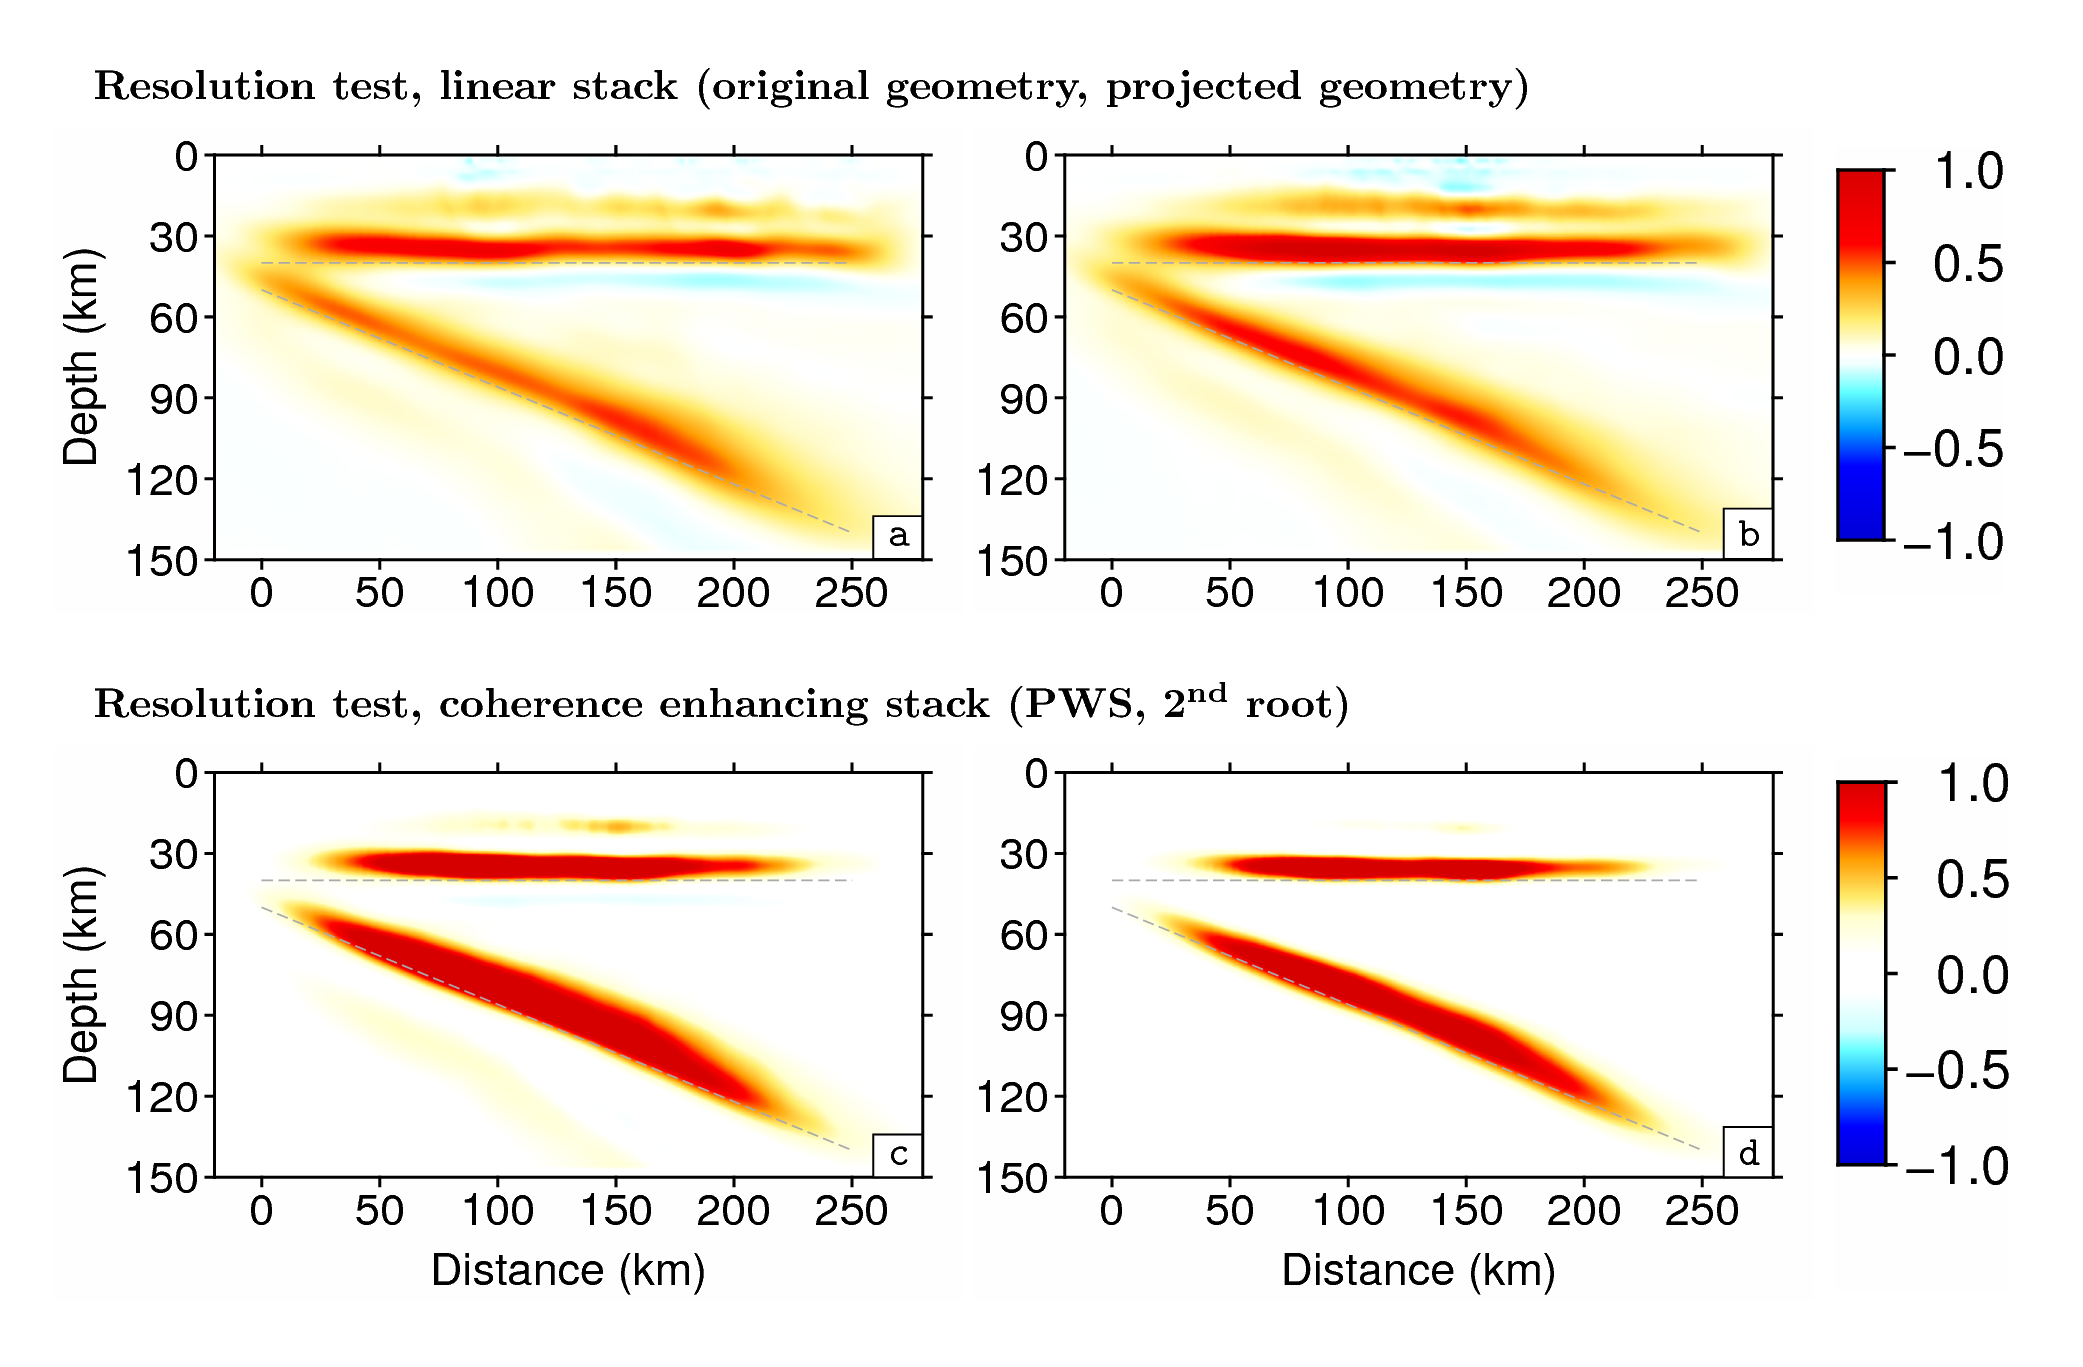
\includegraphics[trim= 0 0 0 0,clip,page=1,scale=.22]
                {../figs/finalfigs/ff11_3.png}
\caption{
Resolution test with a 3 layer synthetic model on the MEDUSA experiment array and source geometry. 
(a) is the linear migration with raw geometry.
(b) to (d) are the linear, phase-weighted and 2\textsuperscript{nd} root stacks with projection, focus and weights (eqs.\eqref{lin},\eqref{pws},\eqref{2rs}, cf. text).
}
\end{figure*}
%-----------------------------------------%
%     F     I     G     U     R     E     %
%-----------------------------------------%

% - - - - - -
% Subsection
% - - - - - -
\subsection{Resolution test}

In order to determine how well our method will be able to perform with this dataset, we first perform a synthetic resolution test on a 2D \hl{subduction} model.
We \hl{generate data for all 52 events recorded at a 35 stations setup as in} the MEDUSA South Line experiment.
\hl{The results will be used to determine} the maximum resolution we can get given the data coverage, maximum frequency and station distribution.
In order to be able to better compare our image with GRT or RTM migrations, we project the data on the imaging line as stated previously.

The data is generated with the Raysum code, and has a main frequency of 0.3Hz.
This corresponds to wavelengths of down to 20km for P-waves and 10km for S-waves, so for the resolution test and the real data we use a 2$\times$2$\times$2km voxel size.
Because the back-scattered S-wave multiples have smaller wavelengths in the model space, we allow for different \hl{frequency bands to be used for the data} in the different modes during the migration.
With an average station spacing of just under 10km, a 30km deep Moho should be easy to retrieve.
%This test will give us the best image possible for this setup, given the frequency band, as it is free of noise and contains only Gaussian peaks. 
To perform this test, we design a three layer reference model described in table1 as MRT.
The first one is the 40km thick overriding crust, then there is a 10\% velocity increase at the Moho and another 10\% velocity increase at the slab interface.
Since the amplitude of the velocity jump is similar for the two interfaces, we expect the two interfaces to show the same scattering potential on the final image.

Results for this synthetic resolution tests with constant frequency range for all modes are shown in fig11.
Fig11a shows the result for the fully 3D imaging principle in eq.\eqref{foc} without projection on the migration line.
The energy focuses on the discontinuities but there is some noise above and just under the Moho with both positive and negative energy values.
There are also some artifacts under the subducted slab.
The features are retrieved at their correct positions but there are along-dip heterogeneities introduced by the uneven spatial distribution of stations.
More specifically, we see along the imaged Moho that there are two regions with higher sensitivity that correspond to the higher density in station coverage.
We individually down-weight the stations that are closer together in an effort to normalize the energy content across the image.

Fig11b shows the result for the linear multi-mode stack with the array projected on the migration line and with individual station weights.
\hl{The discontinuities are highlighted more finely} and there are less along-dip variations.
\hl{Nevertheless,} there are still some remaining artifacts, especially around the over-riding Moho.
Fig11c shows the result for the phase-weighted stack from eq.\eqref{pws} with station weights and the projection.
There are \hl{fewer} artifacts around the Moho \hl{than with the linear stacking} but the spurious streak under the slab persists.
%Also we note that the edges of the imaged discontinuities do not go as far as in fig10b and that the energy is better focused.
Fig11d shows the result for the 2\textsuperscript{nd} root stacking with the individual station weights and the projection.
There are practically no artifacts left around both the Moho and the subducted slab.
\hl{The discontinuities are defined even more finely than with the phase-weighted stacking and the over-riding Moho now appears as a separate feature from the dipping slab.}

\hl{This synthetic example shows that our method is capable of retrieving a good amount of information from the MEDUSA experiment geometry.
The three stacking methods show good results and are efficient at removing most of the spurious energy from the final image.
We expect to retrieve both flat and dipping discontinuities in the data and are confident that we can recover the structure properly in the field data using the multi-mode algorithm.}

%-----------------------------------------%
%     F     I     G     U     R     E     %
%-----------------------------------------%
\begin{figure*}[t]
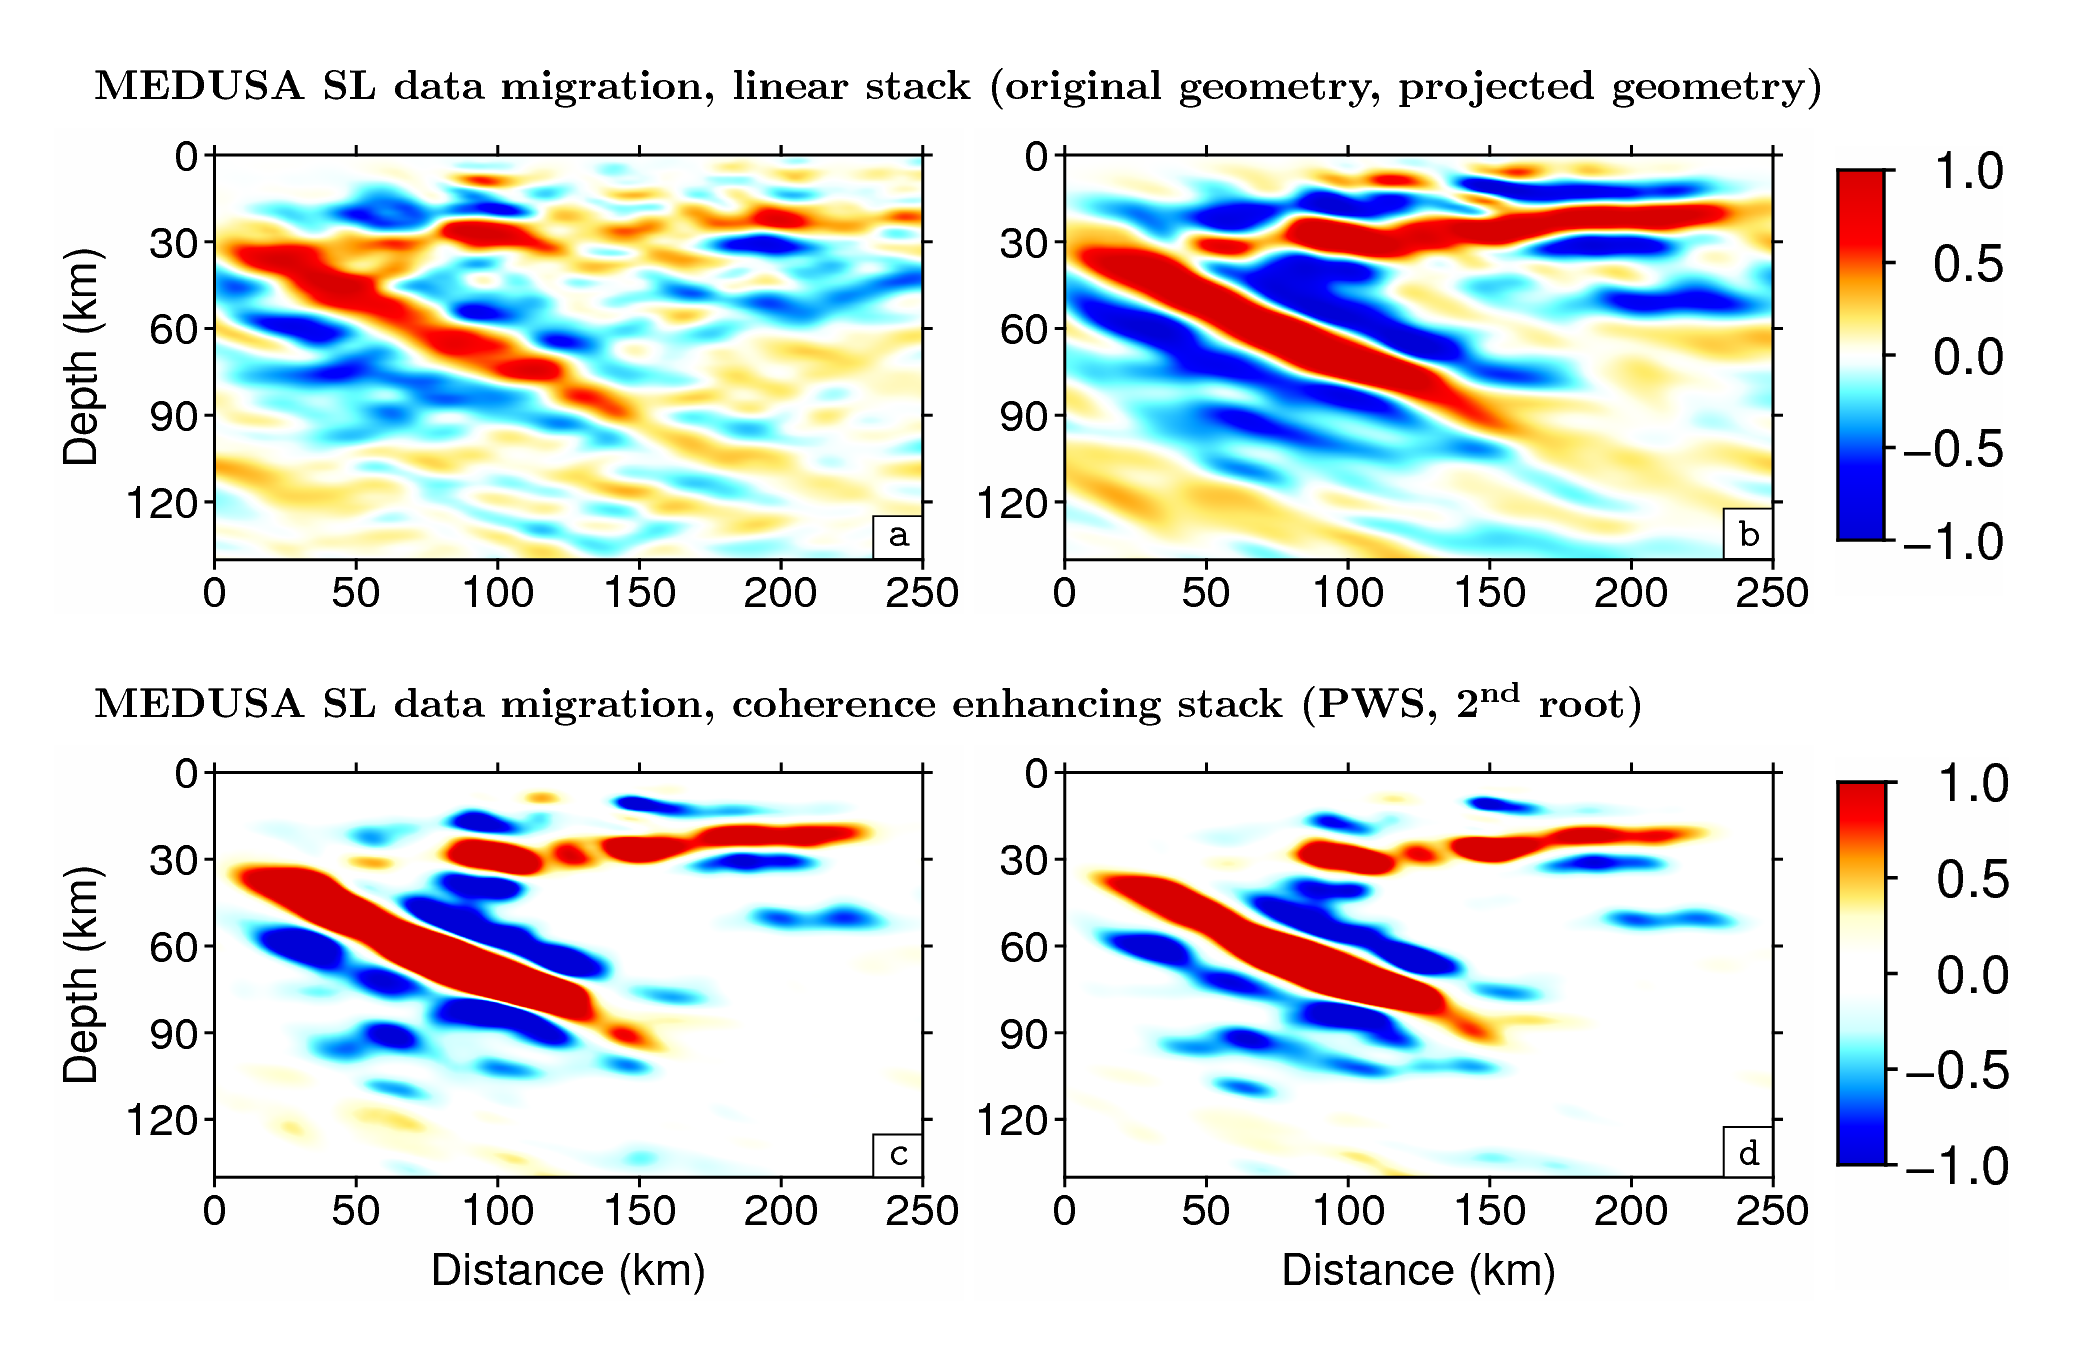
\includegraphics[trim= 0 0 0 0,clip,page=1,scale=.22]
                {../figs/finalfigs/ff12_3.png}
\caption{
Images obtained with the multi-mode migration on the MEDUSA experiment dataset \citep{pear_jgr_12}. 
(a) to (d) correspond to the same imaging principles as figures 11a to 11d respectively.
The over-riding Moho, the subducting crust upper and lower limits are clearly defined. 
}
\end{figure*}
%-----------------------------------------%
%     F     I     G     U     R     E     %
%-----------------------------------------%

% - - - - - -
% Subsection
% - - - - - -
\subsection{Field data migrated sections}

The migrated sections are presented in fig12.
The background velocity model for the migration is the same 1D model as the one used by \citet{pear_jgr_12} and is described in table1 as MPKDM.
\hl{Based on the results from the resolution test, we apply the following treatement to the data to enhance the imaging quality.}
Because of the difference in resolution power between the four modes, we \hl{filter the data in} different frequency bands.
\hl{This helps} to maximize the coherence on the final images.
We filter the data between 0.03Hz and 0.5Hz for the PS and PpP data and between 0.03Hz and 0.3Hz for the PpS and PsS data.
\hl{As we showed in the resolution test, we obtain the best images when we take inter-station spacing into account.
Therefore, we} down-weight the \hl{data from the} stations that are closer together to homogenize the energy content on the cross-section in fig12b to 12d.

The \hl{results obtained with the different stacking methods} are overall comparable to previous results by e.g. \citet{pear_jgr_12}.
\hl{Two main features can be observed in the migrated sections: (1) a 25 km (NE) to 35 km (SW) deep over-riding Moho and (2) a 12km thick, 18$^{\circ}$ north-eastwards dipping subducted crust.}
\hl{The Moho signal disappears close to the slab interface, whereas the subducting crust signal disappears} at 85km for the upper limit and 100km for the lower limit.
Some coherent low-velocity signals are also visible in the mantle wedge.
\hl{In particular, we observe two negative patches under the over-riding Moho at 35 and 55km above the part where the dipping signals disappear} and close to the Sousaki volcano.

\hl{We shall now describe each image individually, starting with} fig12a.
It shows the linear multi-mode stack for the raw 3D geometry, similar to fig11a.
Here the over-riding Moho and the subducting crust are visible but the image is noisy.
There is no clear signal associated with the mantle wedge.
\hl{Next,} fig12b shows the result for the linear stack \hl{with data that} has been projected on the migration line and with the individual station weights, similar to fig11b.
\hl{In this case the over-riding Moho} appears clearly as a linear feature and much of the noise has disappeared.
The slab signature is also more linear \hl{than on fig12a}, with a constant thickness.
Some structures appear in the mantle wedge at 35km and 55km above the region where the dipping signals disappear.
\hl{Lastly,} fig12c and 12d show the results for the phase-weighted stack and 2\textsuperscript{nd} root stack respectively.
Colors have been saturated to emphasize the coherent structure.
The two images are very similar.
The over-riding Moho is separated in two larger patches with smaller scattering intensity in between.
The bottom and top of the \hl{subducting crust} are clearly isolated from their surroundings and there is less noise in the slab.
\hl{The dipping signal is probably lost at depth} due to eclogitization as explained by \citet{pear_jgr_12}.
We acknowledge that we cannot interpret amplitudes in our images in terms of velocity contrast $\delta \beta / \beta$ \hl{using our method.
However,} we find that the three main discontinuities, namely the top of the subducting crust, the slab Moho and the over-riding Moho, have approximately the same scattering potential in our image.
\hl{This roughly translates into the same changes in elastic properties, which is coherent with the previous GRT images} \citep{pear_jgr_12}.

% - - - - - -
% Subsection
% - - - - - -
\subsection{Discussion}

%  -  -  -  -  -
% Subsubsection
%  -  -  -  -  -
\subsubsection{Fluids and melt under Sousaki Volcano}

Our images resemble closely the ones obtained previously with the same dataset by \citet{pear_jgr_12}.
\hl{However, there are} two main differences between \hl{these previous images and ours.}
\hl{First,} we do not recover the same variation in thickness at 40km depth in the subducting crust.
The signal for the suducting crust starts at 30km depth and stays approximately 12km thick until the signal disappears at 90km depth.

\hl{Second,} our image presents two negative patches under the over-riding Moho that we will examine in detail.
\hl{These features} could correspond to \hl{zones of} partial melting or magma accumulations, \hl{similar to what has been propsed in other} settings such as the Cascadia Subduction Zone \citep{mcga_nat_14,wann_ggg_14}.
\hl{The melt} is inferred to be due to dehydration of the slab occurring during the gabbro-to-eclogite transition and the serpentine breakdown in the deeper part of the slab.
\hl{These two reactions release fluids that can migrate in the mantle wedge where they lower the solidus of mantle peridotites and cause partial melting.}
\hl{The melt} can appear and stagnate \hl{in the mantle wedge} because of thermal state of the mantle wedge.
\hl{The central part of the mantle wedge is warmer than its surroundings due to the intrusion of cold subducted material,} and analytical studies predict a local maximum in temperature in the lower part of the mantle wedge, approximately where we see the deepest negative patch \citep{mcga_nat_14}.
\hl{The idea of fluid and melt presence in this region of the subduction zone is corroborated by studies that found potential} fluid pathways from the subducting upper mantle that arrive under the Sousaki volcano where we see these two patches \citep{gala_tphy_05}.

%  -  -  -  -  -
% Subsubsection
%  -  -  -  -  -
\subsubsection{Advantages and drawbacks of the method}

In this paper, we presented our fully 3D prestack migration method, and illustrated it with synthetic examples.
Here we will shortly discuss the advantages and drawbacks of our method compared to other scattered wave studies.

Migration methods such as ours can be compared to pure inversion approaches as they are designed to extract different information from the same data.
Study of the Earth through inversion of scattered waves has been done in many fashions.
Scattered waveforms can be used in full waveform inversions \citep[P-wave coda waveform inversion,][]{fred_gji_04} or in joint inversions with surface waves and other body waves \citep[e.g.,][]{bodi_gji_16}.
However this is very expensive and does not provide the high resolution power of migration methods.

Compared to classic CCP migrations, our method exhibits close to no artifacts when dealing with dipping interfaces and laterally varying media.
In our method we compute the arrival times of the different scattered phases in a tomographic 3D reference model.
Doing so allows us to make no assumption of the scattering strucutre that we want to image.
In this regard our method performs better than classic CCP stacking, which uses the horizontal interface assumption to stack all the traces and speed up the depth mapping of the scattering information \citep{duek_jgr_97}.
This limitation can be partially adressed by wave-number filtering for example \citep[one-way wave equation][]{chen_jgr_05}.
This improves the imaging quality of CCP but is still limited by artifacts which our method does not exhibit at all.
The biggest drawback compared to these poststack methods is computation time as we need to map energy back at depth in three dimensions and for every trace independantly.

Compared to more elaborate imaging methods that get rid of the horizontal interface assumtion altogether, we are limited to migration of scattering potential and cannot distinguish density from velocity.
Methods like the GRT migration \citep[e.g.,][]{bost_jgr_01} or the RTM \citep[e.g.,][]{burd_gji_13} recover elastic parameter perturbations across scattering interfaces using inversion techniques.
The drawback here is that this makes them computationally expensive and mostly limits them to 2D applications.
We took a different approach as we do not include any inversion for elastic parameters which allows us to reduce computation time.
This means that we can only map scattering potential and impedance contrasts at depth.
In other words, we choose to image pure structure over detailed elastic parameters, which is one of the major limitations of our imaging principle.

Similar to what is done in these methods, we use three component RFs.
The information gained from three component data allows for more robust imaging as any incoherent feature on a single component gets attenuated and coherent scattering get enhanced.
This step up in imaging quality is only possible because we take the physics of scattering into account.
In our method, this is done with scattering patterns.
%We use them to estimate the potential scattering intensity at each point with simple analytical formulae and then compare that value with what is recorded on the RFs.
They allow us to automatically process data from all slownesses and back-azimuth without worrying about polarity and amplitude issues.
This way of dealing with scattering intensities is similar to what is done in GRT, and is faster than the full wavefield computations that are used in the RTM methods.

Adapting Kirchhoff migration into an inversion problem for passive seismology was pioneer by \citet{wils_jgr_05} with the Regularized Kirchhoff migration, but some compromises had to be made.
In order to speed up the computations and make a Kirchhoff imaging principle based inversion viable, the arrival times were computed in a one 1D reference velocity model.
This means that the authors loose imaging capability in the case of large lateral variations such as the ones we can see from tomographic models in subduction zones.
By computing the arrival times with a fully 3D scheme, we are able to tackle even the strongest 3D effects.
This is done at the expense of some computational efficiency, but the overall cost is reduced by the introduction of the fast marching method \citep[FM3D,][]{deko_gji_06}.
Using a 1D reference model to speed up computations has also be done in GRT \citep{wang_jgr_16}.

\citet{wils_jgr_05} also implemented and discussed a multi-mode migration.
As showed in section 3, taking not only the transmitted PS mode into account but also the back-scattered PpP, PpS and PsS modes largely improves the imaging quality.
We proved that it is a powerful tool to avoid misinterpreting a spurious LAB.
Multi-node algorithms have also been adapted for 2D CCP \citep{tauz_epsl_16} and GRT migration \citep{bost_jgr_01} and consistently show clear improvements both in synthetic and field data applications.
The only sensible drawback for the multi-mode migration is that it theoretically multiplies the computational time by the number of modes used.
In practice, that coefficient is lower because many of the calculations for a given scattering mode can be used in the other modes.
In our case, we use four different modes and three independant stacking methods but the migration only takes about twice as long as just the PS migration, which is the most used scattering-mode in single mode studies.
Altogether, our method is very similar to recent developpements by e.g., \citet{hans_ggg_17}.

%  -  -  -  -  -
% Subsubsection
%  -  -  -  -  -
\subsubsection{Towards fully three dimensional settings}

\hl{Though our application to field data consists of a 1D array and a 2D slice, it not showcase the benefit of our fully 3D approach.}
However, there are two encouraging points that validate our method as a powerful tool to study the Earth’s interior.
First, we show that when performing the same processing to the data than 2D GRT we get a similar image with our fully 3D imaging principle.
This shows that our method is {\textit{a minima}} as powerful as the GRT migration to \hl{image} the underlying structure of subduction zones in terms of scattering potential.
Second, we show in fig11a and fig12a that by using the original station distribution, which deviates slightly from a 1D array, we can still recover the main features observed by authors of previous studies in the region.
This \hl{suggests} that our imaging method will also provide \hl{robust} imaging power in fully 3D applications. 

%In order to benchmark our method, we first conduct a series of synthetic tests in challenging scenarios and retrieve structure acurately.
%Then we compare our images to the ones obtained in \citet{pear_jgr_12} and see that they are very similar.
%These tests in 2D and 3D settings give us confidence in that our method will be able to recover fine structure in more complex settings, particularly with 2D regional arrays such as USArray.
%So far the test on 2D geometries shows that our method works as well as others scheme that were specifically designed for this case.
%However our method is fully 3D and this means that we can take advantage of much more than those methods.

%Future work includes testing our method in fully 3D geometries, using fully 3D synthetics.
%We also note that we could compare our methods to those of \citet{pavl_cg_11} and \citet{hans_ggg_17}, the latter being especially close to ours.

%---------
% Section
%---------
\section{Conclusions}

In this study, we designed a new method to \hl{process} Receiver Functions and recover the three dimensional distribution of scattering structure in the Earth.
In order to overcome the drawbacks of both fast CCP methods (that rely on the assumption that the underlying discontinuities are horizontal), and complex Reverse-Time Migration and Generalized Radon Transform migrations \hl{(that are too computationally expensive to be run in fully 3D settings)}, we designed a new computationally efficient fully 3D multi-mode Kirchhoff migration. % that does not need full wavefield calculations.

We adapted the Kirchhoff method from reflection to transmission scattering and applied it to passive seismology.
We expanded the work done by \citet{cheng_gji_16} to include three component data and free surface multiples into an efficient multi-mode migration by computing the travel times for all scattered phases using the FM3D software.
We use three component RFs, 3D scattering patterns and coherence filters to extract the information from the fully 3D data.
We explicitly describe the imaging principles that we use in our migrations.

These imaging principles are tested in challenging and realistic synthetic cases, using the Raysum package.
They recover scattering structures with minimal artifacts in all tested cases, and allow to take lateral heterogeneities into account with reasonable computational time.
Our \hl{fully 3D} method has a similar cost to 2D GRT.

Using data from the MEDUSA experiment in the Hellenic subduction zone, we show that our method performs correctly on field data as well.
The images we obtain are similar to the ones obtained with a 2D GRT migration and serve as a benchmark for our imaging method.
Moreover, it reveals details about the presence of low velocity layers under the European continental Moho and in the mantle wedge that can be associated with partial melting and fluid pathways revealed in magnetotelluric studies.

\hl{The passive multi-mode 3D Kirchhoff migration} method will prove useful in complex settings where lateral variations play a large role and has the potential to help seismically highlight observables from other fields such as fluid pathways in magnetotellurics.

%---------
% Section
%---------
\section*{Acknowledgements}

We want to thank Jean Virieux and Benoit Tauzin for helpful discussion about the methodological developements and Hellenic Subduction Zone image interpretation respectively.
This work was funded by the European Union’s Horizon 2020 research and innovation programme under Grant Agreement No. 716542.

\selectlanguage{english}
\bibliographystyle{agsm}
%\bibliographystyle{plain}
\bibliography{Biblio_article1.bib}



%\end{multicols}

%\clearpage
%
%
%%---------
%% Section
%%---------
%\section*{Figures}
%
%\begin{figure}[H]
%%\includegraphics[trim= 0 0 0 0,clip,page=1,scale=.2]
%%                {../figs/finalfigs/ff1_2.png}
%\caption{
%Schematic illustration along a 2D profile of the 3D Kirchhoff prestack imaging principle. 
%The incoming P-waves (solid lines, red background isochrone lines) and scattered S-waves (dashed lines, green background isochrone lines) arrival times are computed at each grid point in the 3D model box and the energy is migrated (blue curve) along a differential isochron that corresponds to the difference in travel time T between the direct wave ($t_D$) and the P wave to the scatterer ($t_P$) added to the S wave to the receiver ($t_S$). 
%This isochron represents all the points in depth in the 3D model space that could account for scattered energy seen at a given time on the RF.
%In the 3D case, the isochron extends as an ellipsoid whose shape depends on the source-receiver geometry and the reference velocity model.
%}
%\end{figure}
%\clearpage
%
%\begin{figure}[H]
%%\includegraphics[trim= 0 0 0 0,clip,3age=1,scale=.18]
%%                {../figs/finalfigs/ff2_2.png}
%\caption{
%Representation of the 3D scattering patterns. 
%The incoming wave arrives from the left-handside along the horizontal axis as either a P-wave oscillating rightwards or an S-wave oscillating upwards, and leaves according to the scattering geometry. 
%The scattering amplitude is represented as distance to the scattering point (center of each plot) and the polarity is represented by color, red being positive and blue negative. 
%Here we can take both forward and back scattering into account. 
%All of them are symmetrical with respect to the horizontal incoming wave propagation axis. 
%Note that $\rho$ perturbations generate mostly back scattering and $\alpha$-$\beta$ perturbations have equal parts of forward and back scattering. 
%The final value for a given scattering geometry is obtained by multiplying the amplitude value by the polarity for that scattering angle.
%}
%\end{figure}
%\clearpage
%
%\begin{figure}[H]
%%\includegraphics[trim= 0 0 0 0,clip,page=1,scale=.2]
%%                {../figs/finalfigs/ff3_2.png}
%\caption{
%2D representation of the complete scattering weights without focussing for the four scattering modes and the three components migration. 
%The row correspond to a given scattering mode and the columns correspond to the three components of the recorded wavefield.
%For the transverse component, because its amplitude is null along the great circle plane, the slice through the 3D model is offset shallower (towards the reader) or deeper (away from the reader) to visualize its amplitude and polarity behaviour better.
%This is what generates the visible polarity reversals at 200km.
%They are obtained by migrating a unit gaussian peak along the isochron for a given scattering mode for a source that arrives under the station from the right-handside. 
%They correspond to the projection of the weights from the scattering patterns at the surface for each recorded component, with blue corresponding to a polarity reversal and red to a preserved polarity.
%}
%\end{figure}
%\clearpage
%
%\begin{figure}[H]
%%\includegraphics[trim= 0 0 0 0,clip,page=1,scale=.2]
%%                {../figs/finalfigs/ff4_2.png}
%\caption{
%Synthetic setup for the tests in figures 5 to 9. 
%Red triangles represent the stations in the array and green stars represent the events. 
%The array is elongated in the along-dip direction and the sources are evenly spaced in backazimuth and assigned a random epicentral distance from 30$^{\circ}$ to 90$^{\circ}$. 
%(a) is a bloc diagram that represents the velocity model for figure 9 (cf. Table 1). 
%(b) is a map view of the array and shows the event distribution for the tests performed in figures 7 to 9.
%For enhanced clarity only half the rows and half the columns of the array are represented.
%}
%\end{figure}
%\clearpage
%
%\begin{figure}[H]
%%\includegraphics[trim= 0 0 0 0,clip,page=1,scale=.2]
%%                {../figs/finalfigs/ff5_2.png}
%\caption{
%Influence of the Scattering Patterns.
%PS migration of the radial component of the RF for a 2D model with a single interface at 40$^{\circ}$ dip and 10\% $\delta V_P$, $\delta V_S$ and $\delta \rho$ perturbations. 
%(a) and (d) correspond to a down-dip source coming from the right-handside, (b) and (e) to an up-dip source coming from the left-handside, (c) and (f) correspond to the stacks of (a+b) and (d+e) respectively. 
%(a) to (c) are migrated without the scattering patterns and show inconsistency in the migrated polarity. 
%(d) to (f) are migrated with the effects of scattering patterns taken into account and show consistent polarity, which improves the stacked image.
%}
%\end{figure}
%\clearpage
%
%\begin{figure}[H]
%%\includegraphics[trim= 0 0 0 0,clip,page=1,scale=.2]
%%                {../figs/finalfigs/ff6_2.png}
%\caption{
%Influence of the three component migration.
%PS migration for a 2D model with a single interface at 40$^{\circ}$ dip and 10\% $\delta V_P$, $\delta V_S$ and $\delta \rho$ perturbations. 
%(a), (d) and (g) correspond to an along-strike source coming from the readers perspective, (b), (e) and (h) to an along-strike source coming from the other direction, (c), (f) and (i) correspond to the stacks of (a+b), (d+e) and (g+h) respectively. 
%(a) to (c) are the radial components of the RFs migrated without the scattering patterns and show cohenrent but relatively low amplitudes compared to figure 5a. 
%(d) to (f) are transverse and vertical components of the RFs migrated without the scattering patterns and show higher energy content but inconsistent polarities. 
%In (g) to (i), the three components of the RFs migrated with the effects of the scattering patterns taken into account.
%%This time we observe a consistent polarity and higher amplitudes, which improves the stacked image.
%}
%\end{figure}
%\clearpage
%
%\begin{figure}[H]
%%\includegraphics[trim= 0 0 0 0,clip,page=1,scale=.2]
%%                {../figs/finalfigs/ff7_2.png}
%\caption{
%Single-mode migrations of three components RF for a 2D model with a single interface at 10$^{\circ}$ dip and 10\% $\delta V_P$, $\delta V_S$ and $\delta \rho$ perturbations. 
%(a) is the PS, (b) the PpP, (c) the PpS and (d) the PsS migrations (cf. text). 
%24 sources regularly spaced in back-azimuth and with 30$^{\circ}$ to 90$^{\circ}$ of epicentral distance were used in the migrations. 
%The four image recover the structure with the correct polarity but are affected by the other modes.
%The spurious migrations are at different locations in each migration.
%}
%\end{figure}
%\clearpage
%
%\begin{figure}[H]
%%\includegraphics[trim= 0 0 0 0,clip,page=1,scale=.2]
%%                {../figs/finalfigs/ff8_2.png}
%\caption{
%Multi-Mode migrations for a 2D model with a single interface at 10$^{\circ}$ dip and 10\% $\delta V_P$, $\delta V_S$ and $\delta \rho$ perturbations.
%(a) Linear, (b) phase-weighted and (c) 2nd root stacks for the multi-mode migration of the 3 component RFs with scattering patterns for 24 sources coming from all azimuths from 30$^{\circ}$ to 90$^{\circ}$ of epicentral distance.
%}
%\end{figure}
%\clearpage
%
%\begin{figure}[H]
%%\includegraphics[trim= 0 0 0 0,clip,page=1,scale=.2]
%%                {../figs/finalfigs/ff9_2.png}
%\caption{
%Single scattering-mode and multi-mode migrations for the 2.5D Subduction Zone (R2DSZ, Table 1).
%The upper 4 images (a=PS, b=PpP, c=PpS, d=PsS) are the 4 migrations for the 4 single-scattering modes (eq.\eqref{foc}). 
%The lower 3 images correspond to the linear (e, eq.\eqref{lin}), phase-weighted (f, eq.\eqref{pws}) and 2\textsuperscript{nd} root (g, eq.\eqref{2rs}) stacked images.
%}
%\end{figure}
%\clearpage
%
%\begin{figure}[H]
%%\includegraphics[trim= 0 0 0 0,clip,page=1,scale=.2]
%%                {../figs/finalfigs/ff10_2.png}
%\caption{
%Resolution test with a 3 layer synthetic model on the MEDUSA experiment array and source geometry. 
%(a) is the linear migration with raw geometry.
%(b) to (d) are the linear, phase-weighted and 2\textsuperscript{nd} root stacks with projection, focus and weights (eqs.\eqref{lin},\eqref{pws},\eqref{2rs}, cf. text).
%}
%\end{figure}
%\clearpage
%
%\begin{figure}[H]
%%\includegraphics[trim= 0 0 0 0,clip,page=1,scale=.2]
%%                {../figs/finalfigs/ff11_2.png}
%\caption{
%Images obtained with the multi-mode migration on the MEDUSA experiment dataset \citep{pear_jgr_12}. 
%(a) corresponds to the array setup, with white triangles representing the stations position from 1 (south-western corner) to 35 (north-eastern corner) and the projecting line in solid black. 
%(b) is the data for one event sorted but station number. 
%(c) is the interpreted data where we highlight the presence of the continental Moho (orange) and the subducting slab (green).
%We differentiate the forward conversions (solid lines) from the free surface mutliples (dashed lines).
%(d) to (g) correspond to the same imaging principles as figures 11a to 11d respectively.
%}
%\end{figure}
%\clearpage
%
%\begin{table}[H]
%%\includegraphics[trim= 0 0 0 0,clip,page=1,scale=.2]
%%                {../figs/finalfigs/ft1_2.png}
%\caption{
%Synthetic models and setups.
%Dip corresponds to the upper interface of the layer. 
%$V_P$ and $V_S$ are given in $km \cdot s^{-1}$ and $\infty$ corresponds to the semi-infinite layer at the bottom of the model. 
%Thickness is taken at the center of the model and corrected for dip.
%}
%\end{table}
%\clearpage
%
%\begin{table}[H]
%%\includegraphics[trim= 0 0 0 0,clip,page=1,scale=.2]
%%                {../figs/finalfigs/ft3_2.png}
%\caption{
%Index of migrated sections with the effects taken into account for each.
%Additional processing corresponds to the projection of the stations along the imaging line in the case of the MEDUSA experiment.
%}
%\end{table}



\end{document}
